\chapter{Registration of Large Models}
The subject area of this paper is the registration of scans taken of a large and structurally complex physical objects. The thesis is set in the context of the full 3D scanning of the Brussels ``Hôtel de Ville'', a current project by LISA. In particular this paper focusses on the registration of long-range scans of the entire building with short-range, high resolution close-up scans of some features of it.


\section{``Hôtel de Ville'' scanning project}
This is a current 3D documentation projection by the the Image research unit of the \emph{Laboratories of Image, Signal processing and Acoustics} (LISA) at ULB. The goal is to create a full 3D model of the ``Hôtel de Ville de Bruxelles'' \footnote{Brussels Town Hall} building. It is a medieval building built in the beginning of the 15th century, with a Brabantine Gothic-style architecture.


\section{Relief point cloud}
As indicated in the beginning, the physical object is imagined as an ensemble of continuous two-dimensional surfaces embedded in three-dimensional space. The point cloud is taken to be a discrete set of points that lie on those surfaces. Because many different kinds of objects can be scanned and good approaches for processing and registering them vary depending on many factors, it is useful to restrict the scope to a particular kind of point cloud.

Therefore only point clouds that model a single, approximatively planar surface are considered. The defining characteristic is how well it can be represented as a height map on a plane $A_P$. Scans of engravings on a stone wall, such as the ``dessus-de-porte'' on figure \ref{fig:hdv_dessus} can for instance be put into this category. This type of surface will be called ``relief'' in this paper.

\subsection{def}
Let $A$ be a plane and $P$ a point cloud, both in the same coordinate system. For each $\vec{p} \in P$, $d(p)$ is the signed orthogonal distance from $\vec{p}$ to $A$, and $\vec{p_A}$ the projection of $\vec{p}$ onto $A$.


\subsection{Artificial relief} \label{sec:art_relief}
To be able to study registration of point clouds, it is useful to generate artificial points clouds that fit into this category and for which exact values of the underlying surface can be computed.

An algorithm was devised to generate artificial relief surfaces, which look as shown on figure \ref{fig:relief_render}.

\begin{figure}[H]
\centering
\begin{subfigure}{.5\textwidth}
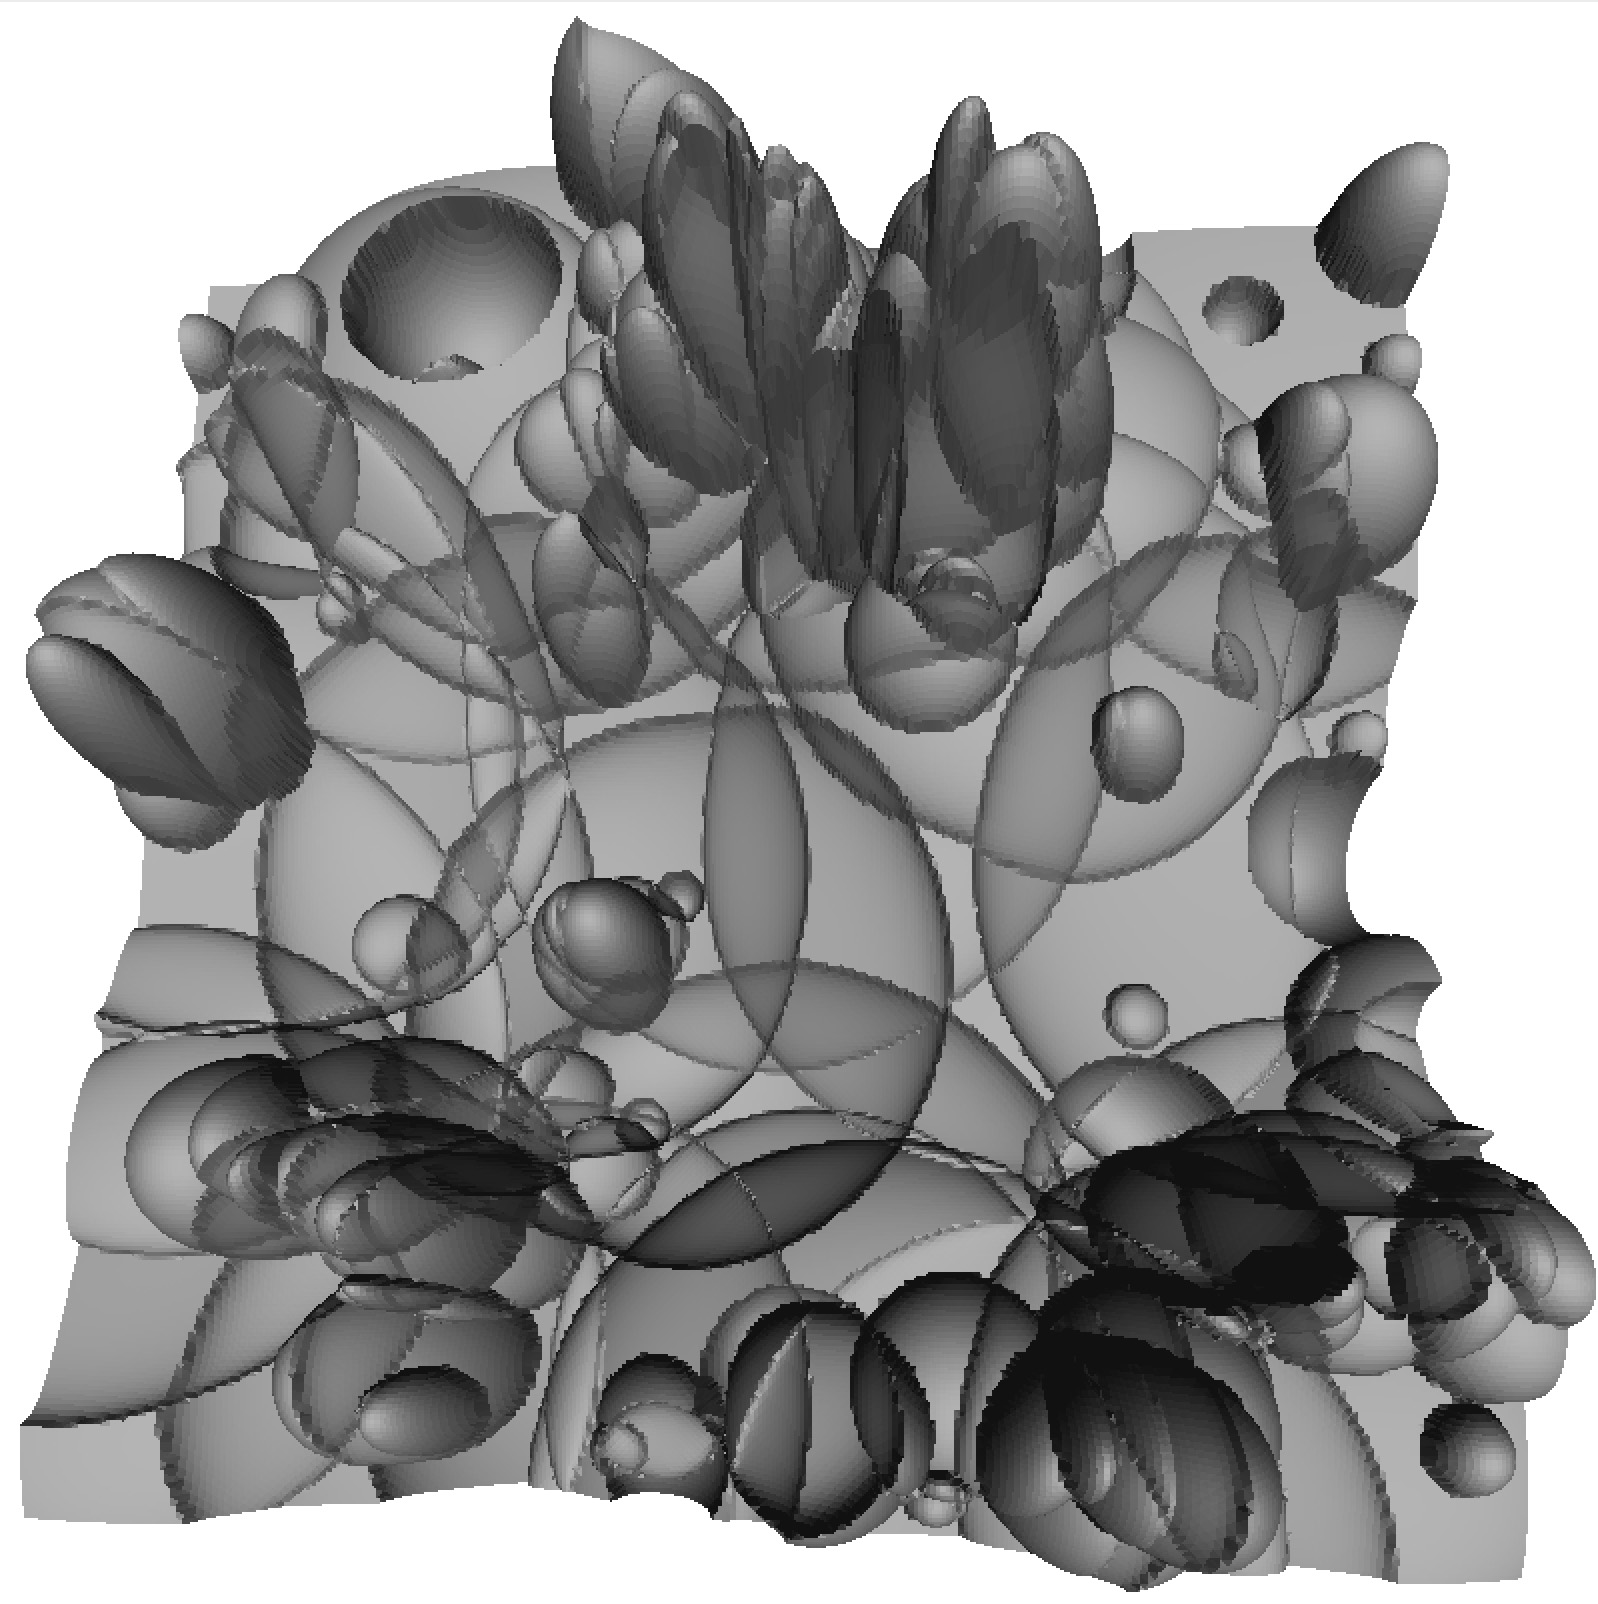
\includegraphics[width=\linewidth]{fig/r1_render2.jpg}
\end{subfigure}%
\begin{subfigure}{.5\textwidth}
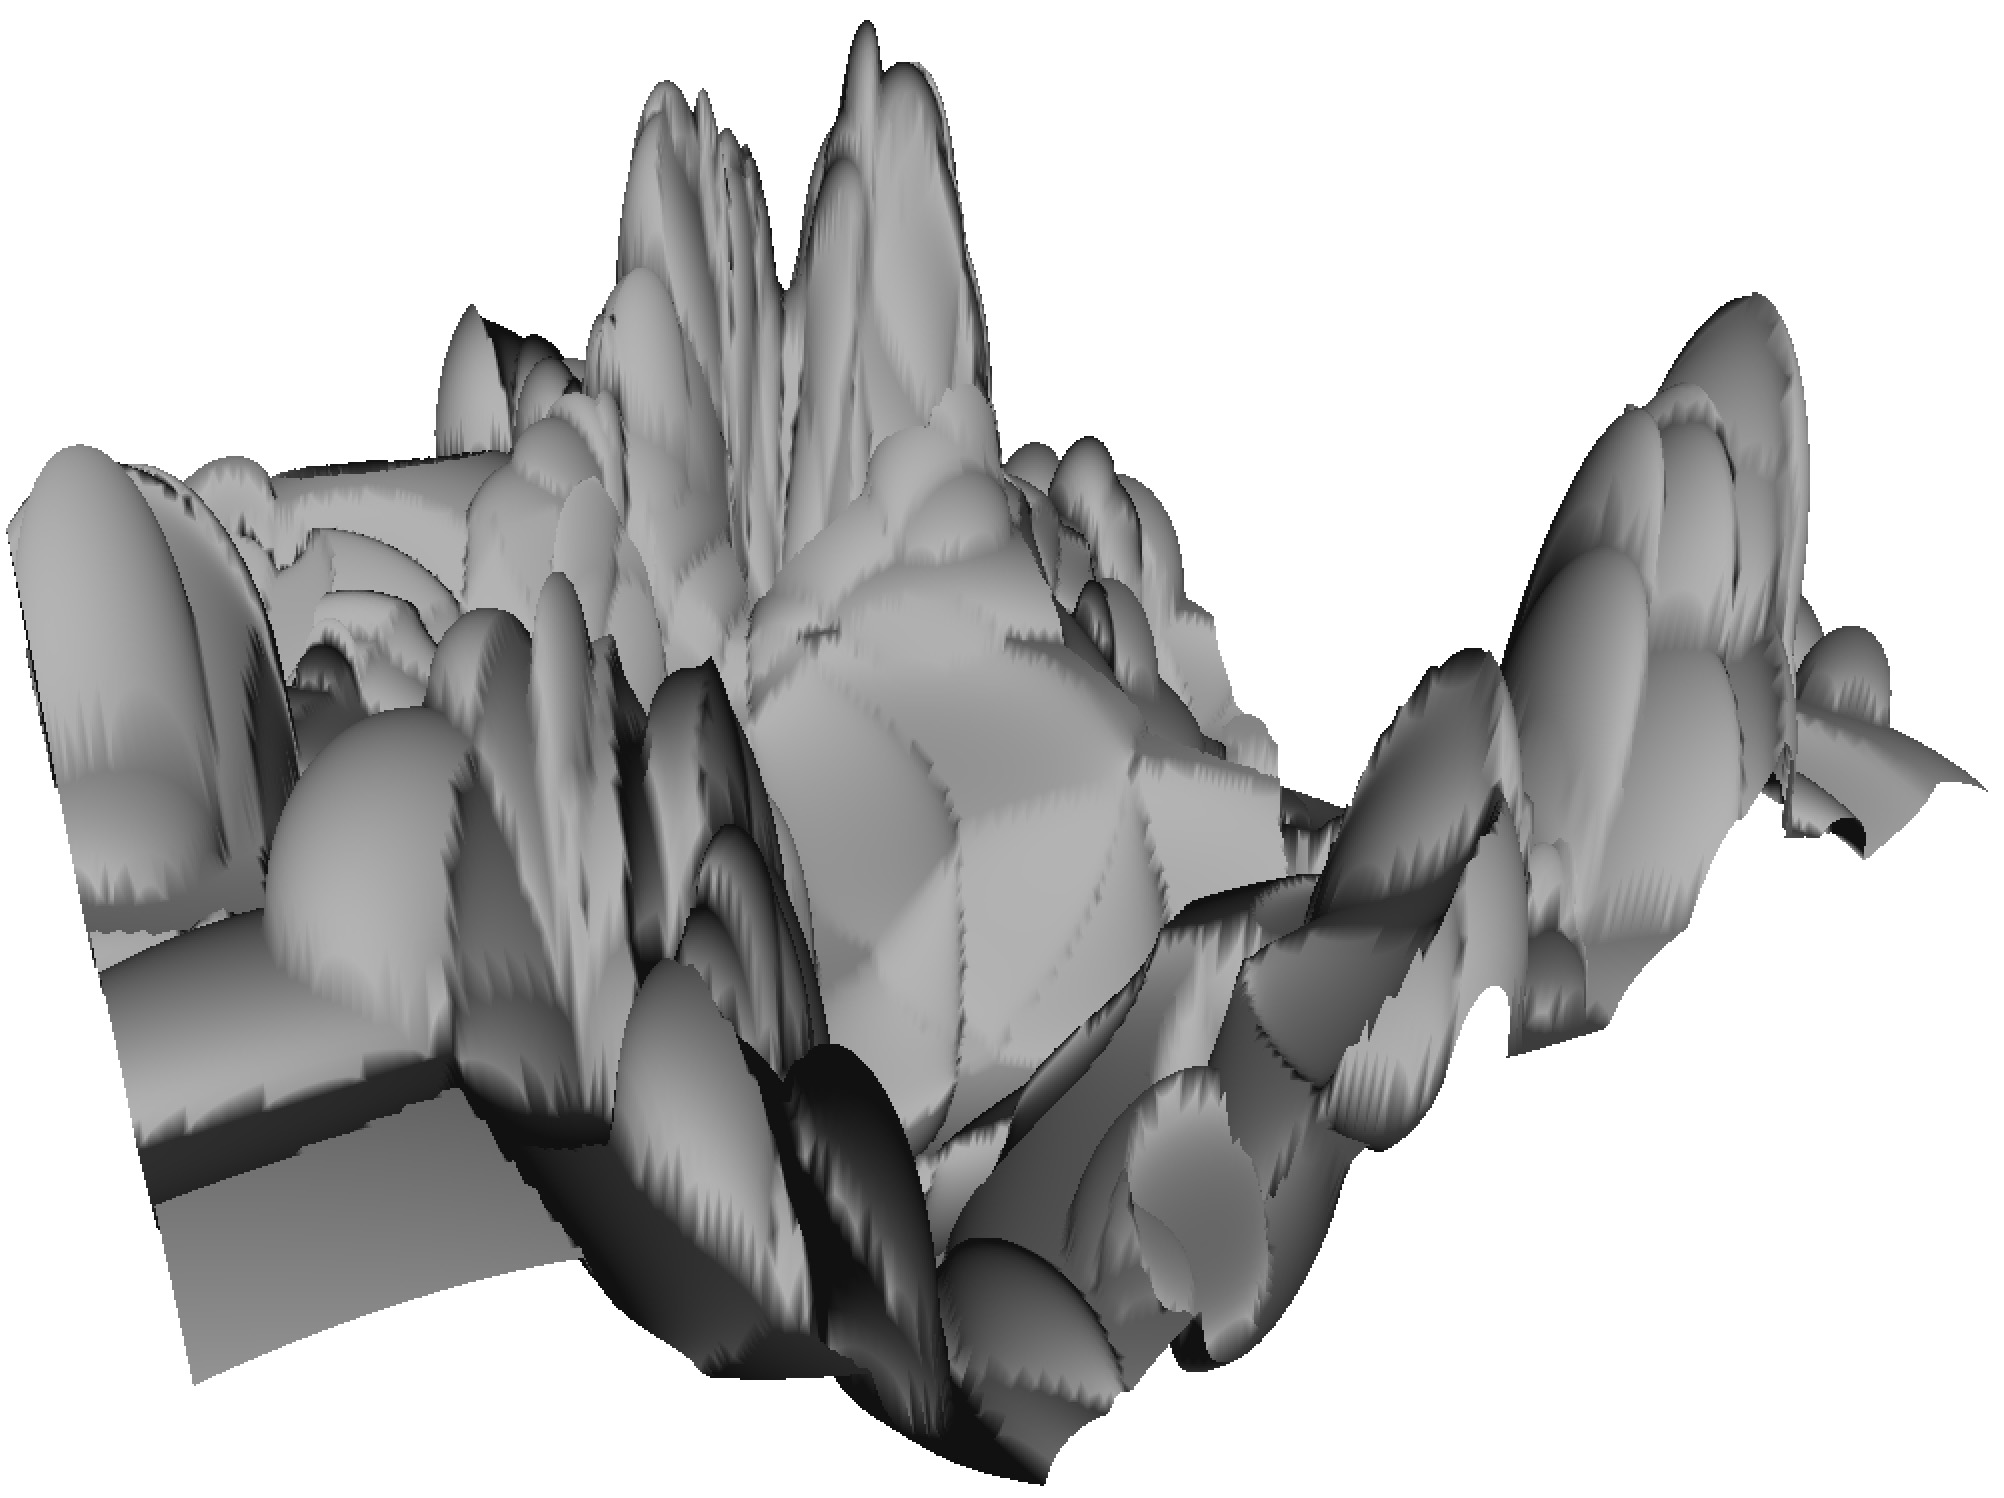
\includegraphics[width=\linewidth]{fig/r1_render1.jpg}
\end{subfigure}
\caption{Artificial relief surface, seen from two view points}
\label{fig:relief_render}
\end{figure}

The entire algorithm is randomized, but can be made deterministic by specifying a seed value for the random number generator. The surface to generate is specified by a \emph{width} $w$, a \emph{height multiplier} $h$, and this seed value.

The generated point cloud is a height map on the XY-plane. Let $z = R[x,y]$ be the $z$ component of the single point with given $x, y$ components. It is defined for $-\frac{w}{2} \leq x,y \leq +\frac{w}{2}$. At first, let $R[x,y] = 0$ for all these points. The result is a square surface of side length $w$.

The algorithm proceeds by pushing randomized ``embossings'' into the surface. The embossings are the shape of a half-sphere distorted in one direction, and is described using the height map formula
\begin{equation}
B_i[x,y] = \pm \, h_i \sqrt{1 - \frac{(x_i - x)^2 + (y_i - y)^2}{r_i^2}}
\end{equation}
A plot of its two-dimensional analogue is shown in figure \ref{fig:relief_B}. $B_i[x,y]$ is set to $0$ for coordinates $x,y$ outside its domain, that is, for $x,y : (x_i - x)^2 + (y_i - y)^2 > r^2$. As a consequence a sharp circular corner is formed around the border.

A fixed number $n$ of embossings are generated with different parameters, and are added to $R$, so that
\begin{equation}
R[x,y] = \sum_{i=1}{n} B_i[x,y]
\end{equation}

The resulting height map will be split into regions $\{(x,y)\}$ where different subsets of $\{B_i\}$ are active. ($B_i$ is active when $(x,y)$ lies in its domain). $R$ has sharp corners at the border points of all $B_i$. As soon as more than one embossing is active in one region, the $z$ coordinate becomes a sum of square roots, producing a complicated shape for both the continuous surface areas and the corners. Its partial derivatives can still easily be calculated analytically, which allows for accurate computation of normal vectors. 

\begin{figure}[h]
\centering
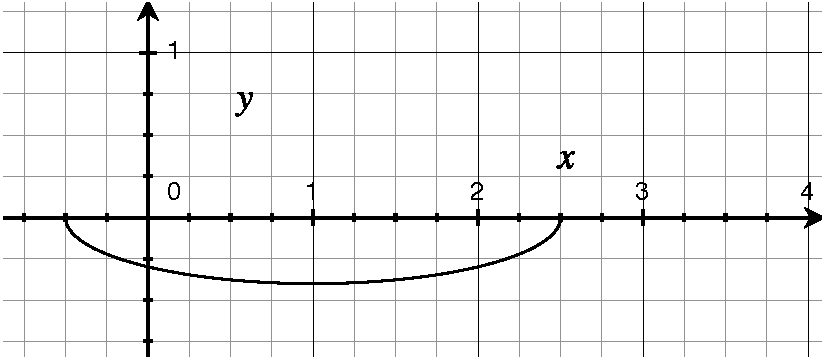
\includegraphics[width=.5\textwidth]{fig/relief_B.pdf}
\caption{2D example for relief embossing, with $h_i = -0.4$, $r_i = 1.5$, and $x_i = 1.0$}
\label{fig:relief_B}
\end{figure}

The radius $r_i$, height $h_i$ and center $(x_i, y_i)$ are randomly chosen for each embossing $B_i$. $x_i, y_i$ are chosen with a uniform distribution in $[-\frac{w}{2}, +\frac{w}{2}]$. The parameters for choosing $r_i$ and $h_i$ are set in such a way that the resulting surface will contain both flat regions and ``spikes'', which occlude parts of the surface when viewed from the side. $h_i$ can be both positive or negative.

\subsection{Point cloud generation}
\subsubsection{Top-down view}
Two ways of generating a point cloud of a relief surface are used. The simplest way is to simply take a set of points $\{ x, y, R[x,y] \}$. It results in a \emph{top-down} view of the surface, as seen by an orthogonal projective camera looking in $-z$ direction. From that view point the model has no occluded surfaces. The $x, y$ coordinates are arranged on a square grid, with a given density $\rho$. Figure \ref{fig:relief_plain} shows an example of such a point cloud, itself projected with a perspective camera.

\begin{figure}[p]
\centering
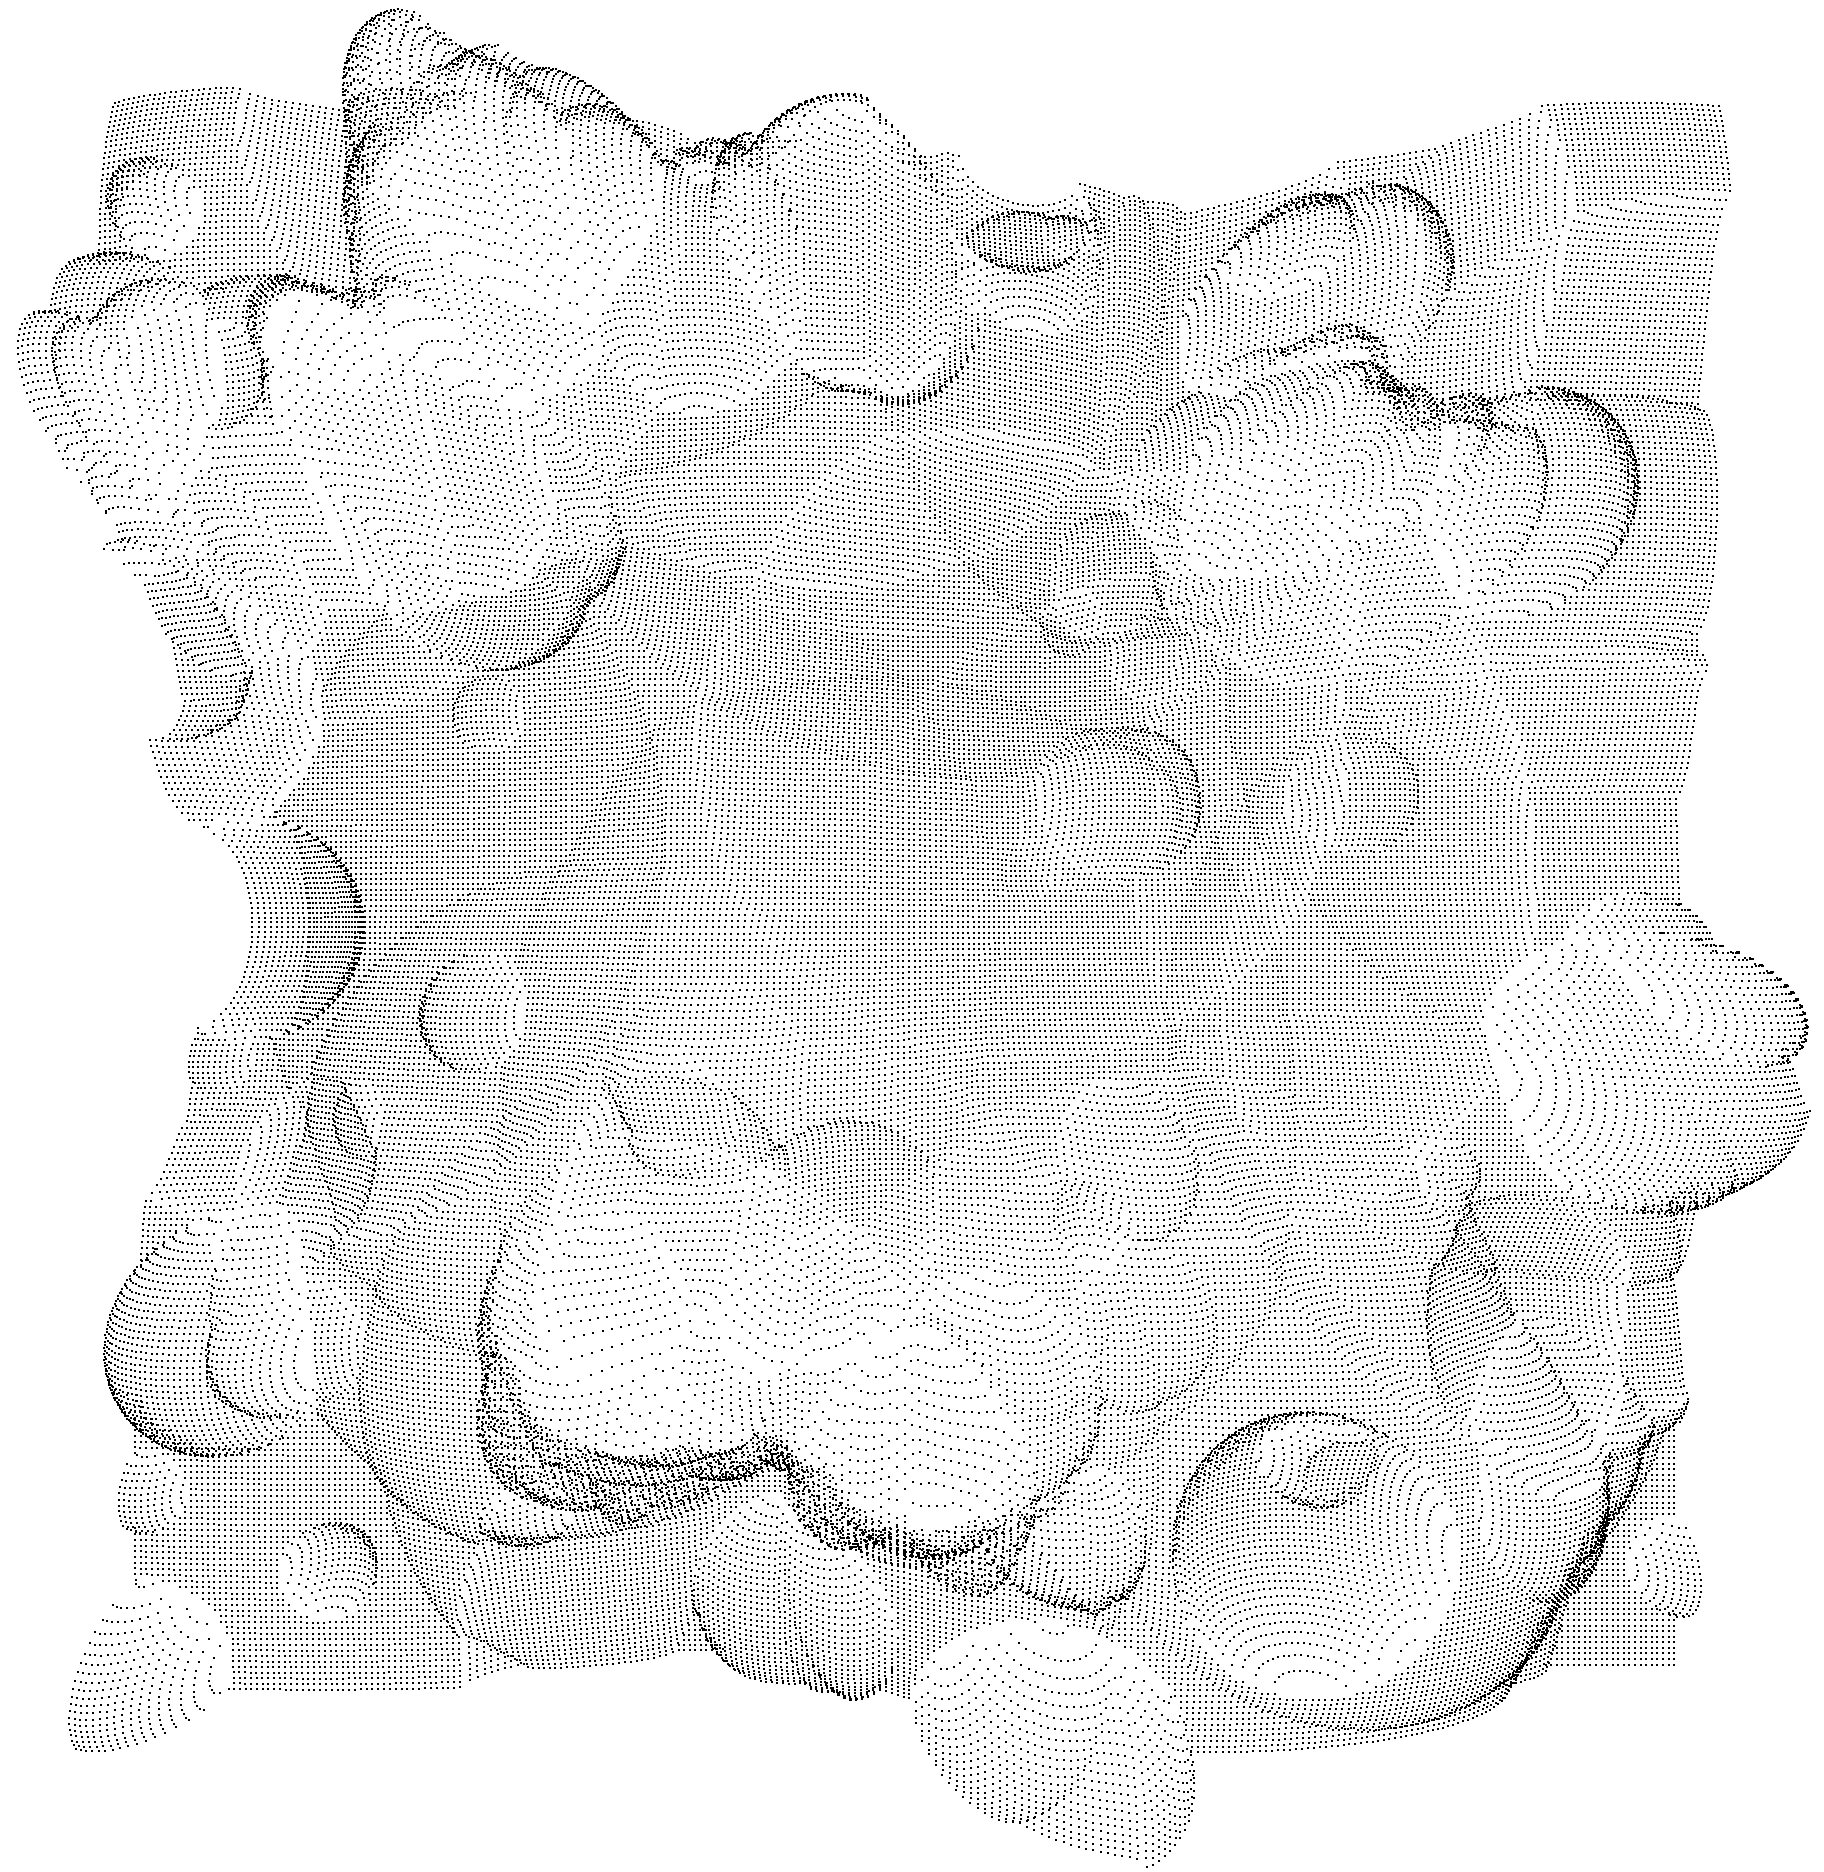
\includegraphics[width=\textwidth]{fig/r1_plain.png}
\caption{Top-down point cloud of relief}
\label{fig:relief_plain}
\end{figure}

\subsubsection{Occluded view}
However the goal of the artificial relief surface was to simulate the kinds of surfaces that occur on real objects, and to get a point cloud with similar properties to a 3D scan of it. So it is important to be able to generate point clouds of the relief as seen from another camera positions, with the occlusions that occur.

A virtual camera is placed near the surface at a given pose, and a range image is generated using it. With an orthogonal projection camera, the point density on the surfaces will remain constant, and with a perspective projection camera, it will decline with distance to the camera.

For the algorithm that creates this range image, a first attempt was to first generate a top-down view point cloud with high enough density, and then generate project that point cloud into a range image as described in \ref{sec:pc_registration}. However, this inevitably leaves points in the occluded areas.

Another attempt was to implement a ray-tracing method that operates on the expression of $R[x,y]$: For each image pixel, calculate the intersections with the view ray and the surface $R$ and take the closest one. However, these intersections cannot easily be calculated analytically. Firstly, the various regions of $R$ with different active embossings must be considered separately. But even on a single such region, multiple intersection points can still occur, and there is no direct closed-form expression for finding them. So a lot of combinatorics and numerical approximation would be required.

Instead, the implemented algorithm generates a mesh of the surface, projects a depth map of it onto image space, and then back-projects the image pixel coordinates into points. Figure \ref{fig:relief_occlusion} shows the resulting point cloud from two view points, the second one near the projection camera pose.

\begin{figure}[h]
\centering
\begin{subfigure}{.5\textwidth}
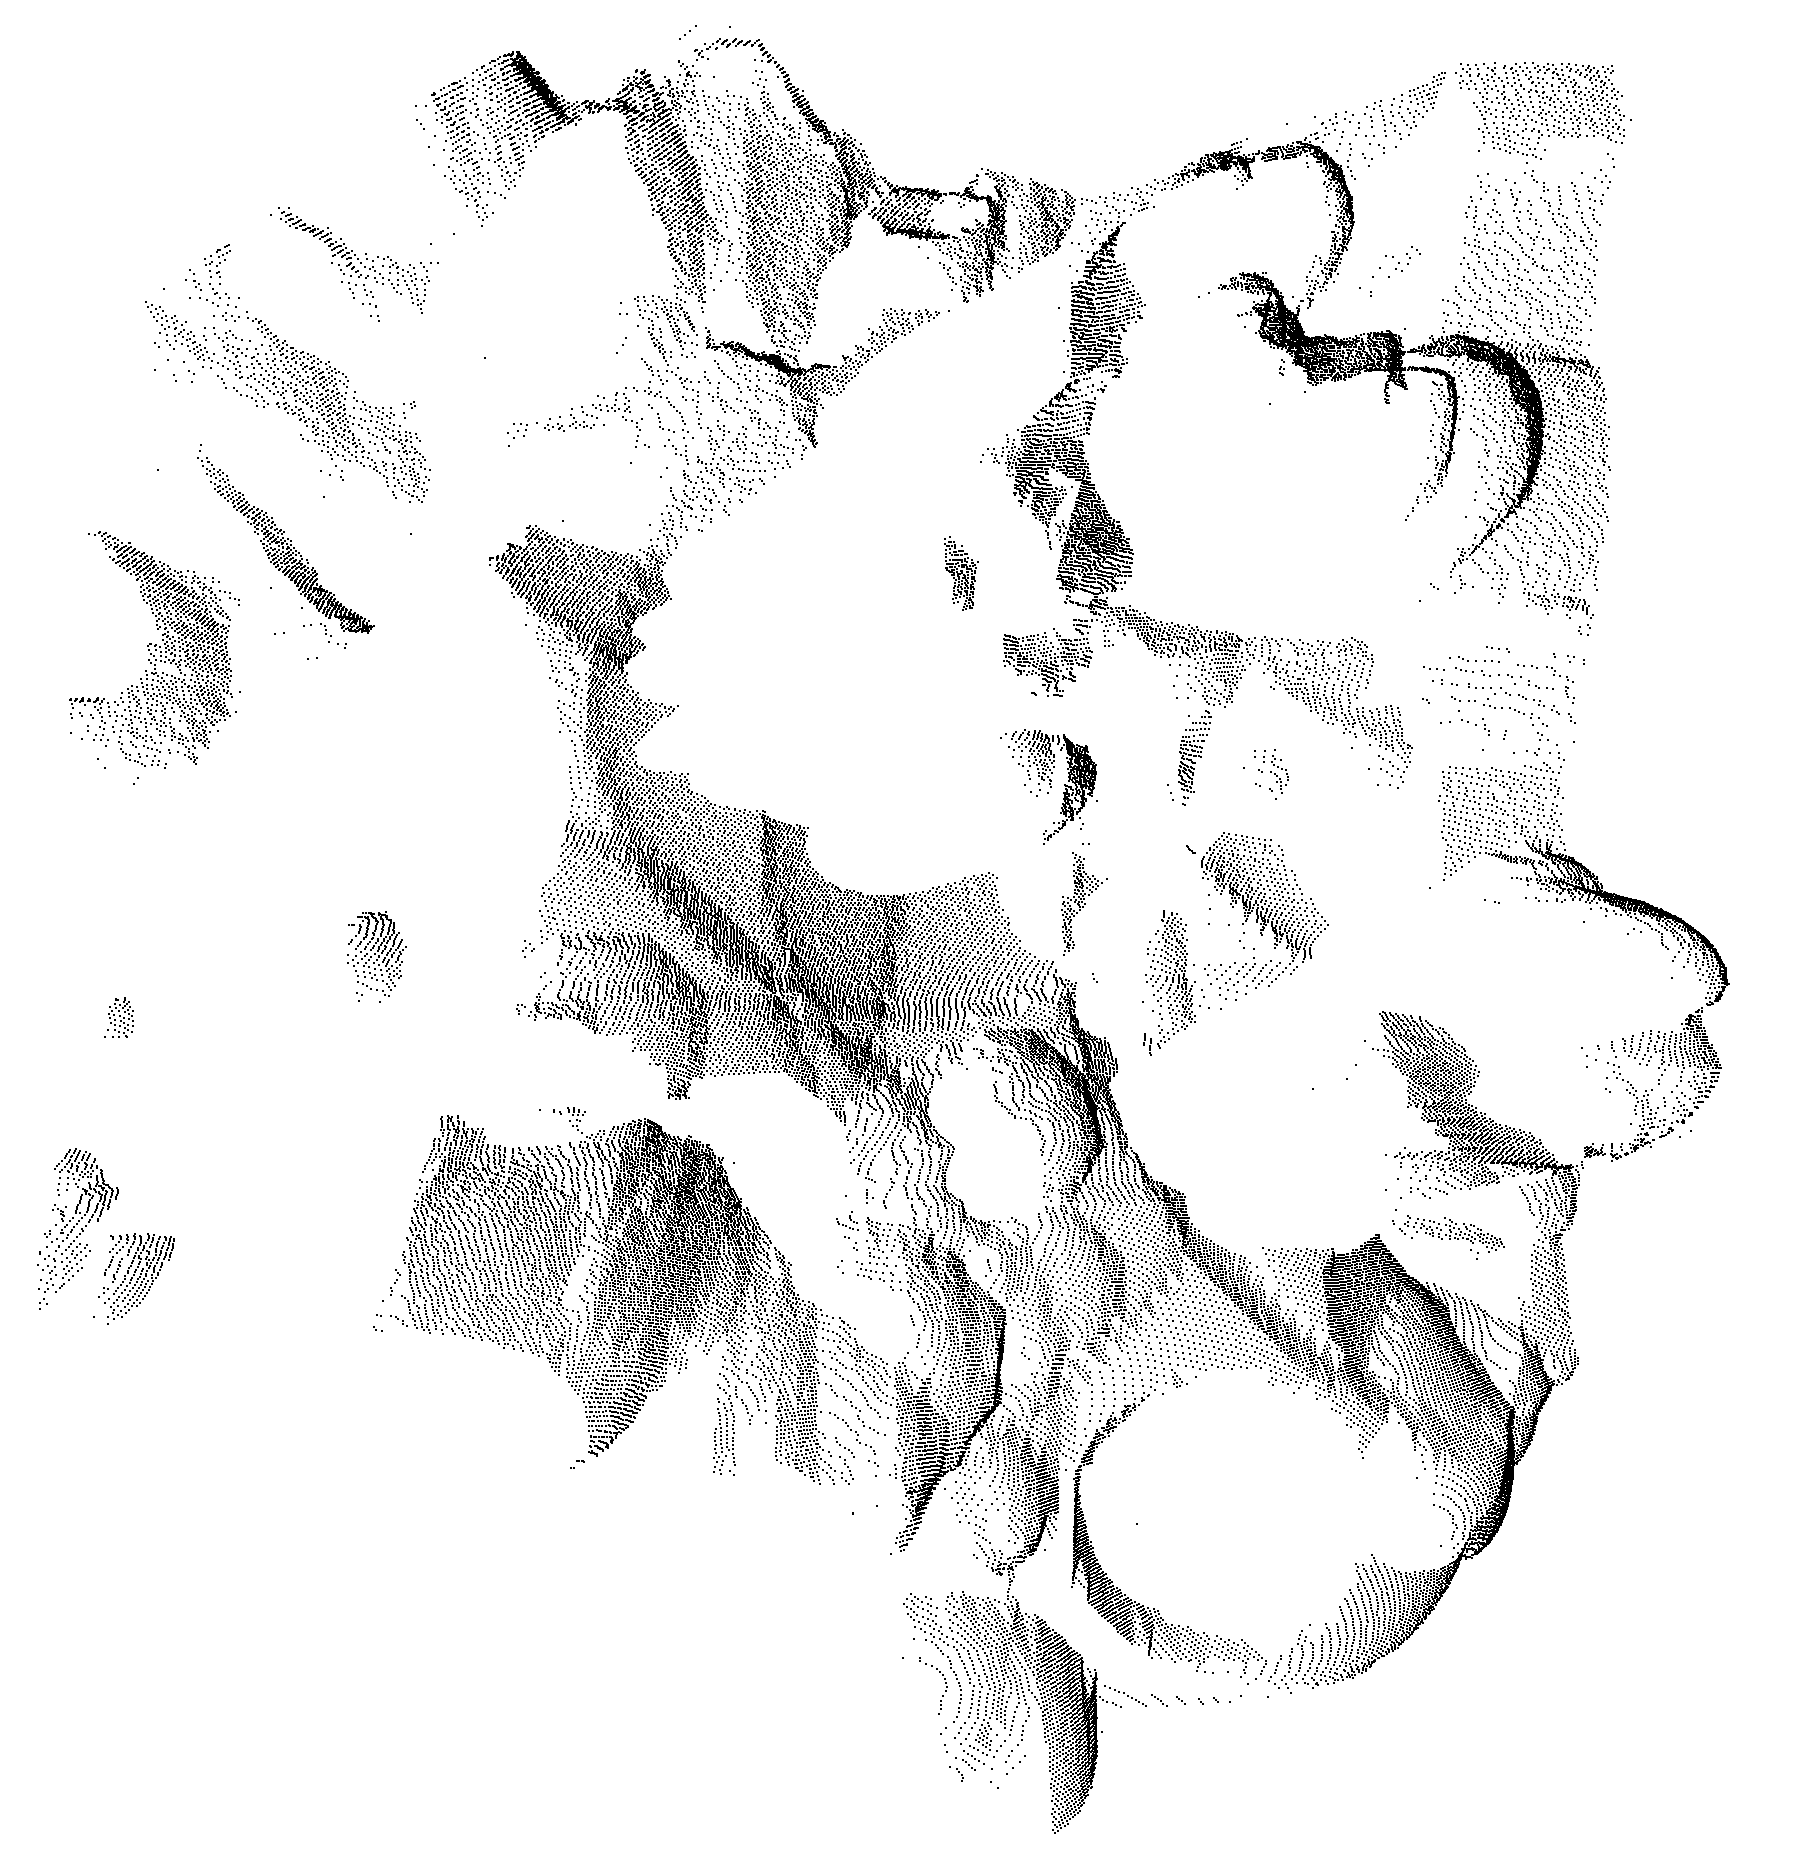
\includegraphics[width=\linewidth]{fig/r1_occlusion.png}
\end{subfigure}%
\begin{subfigure}{.5\textwidth}
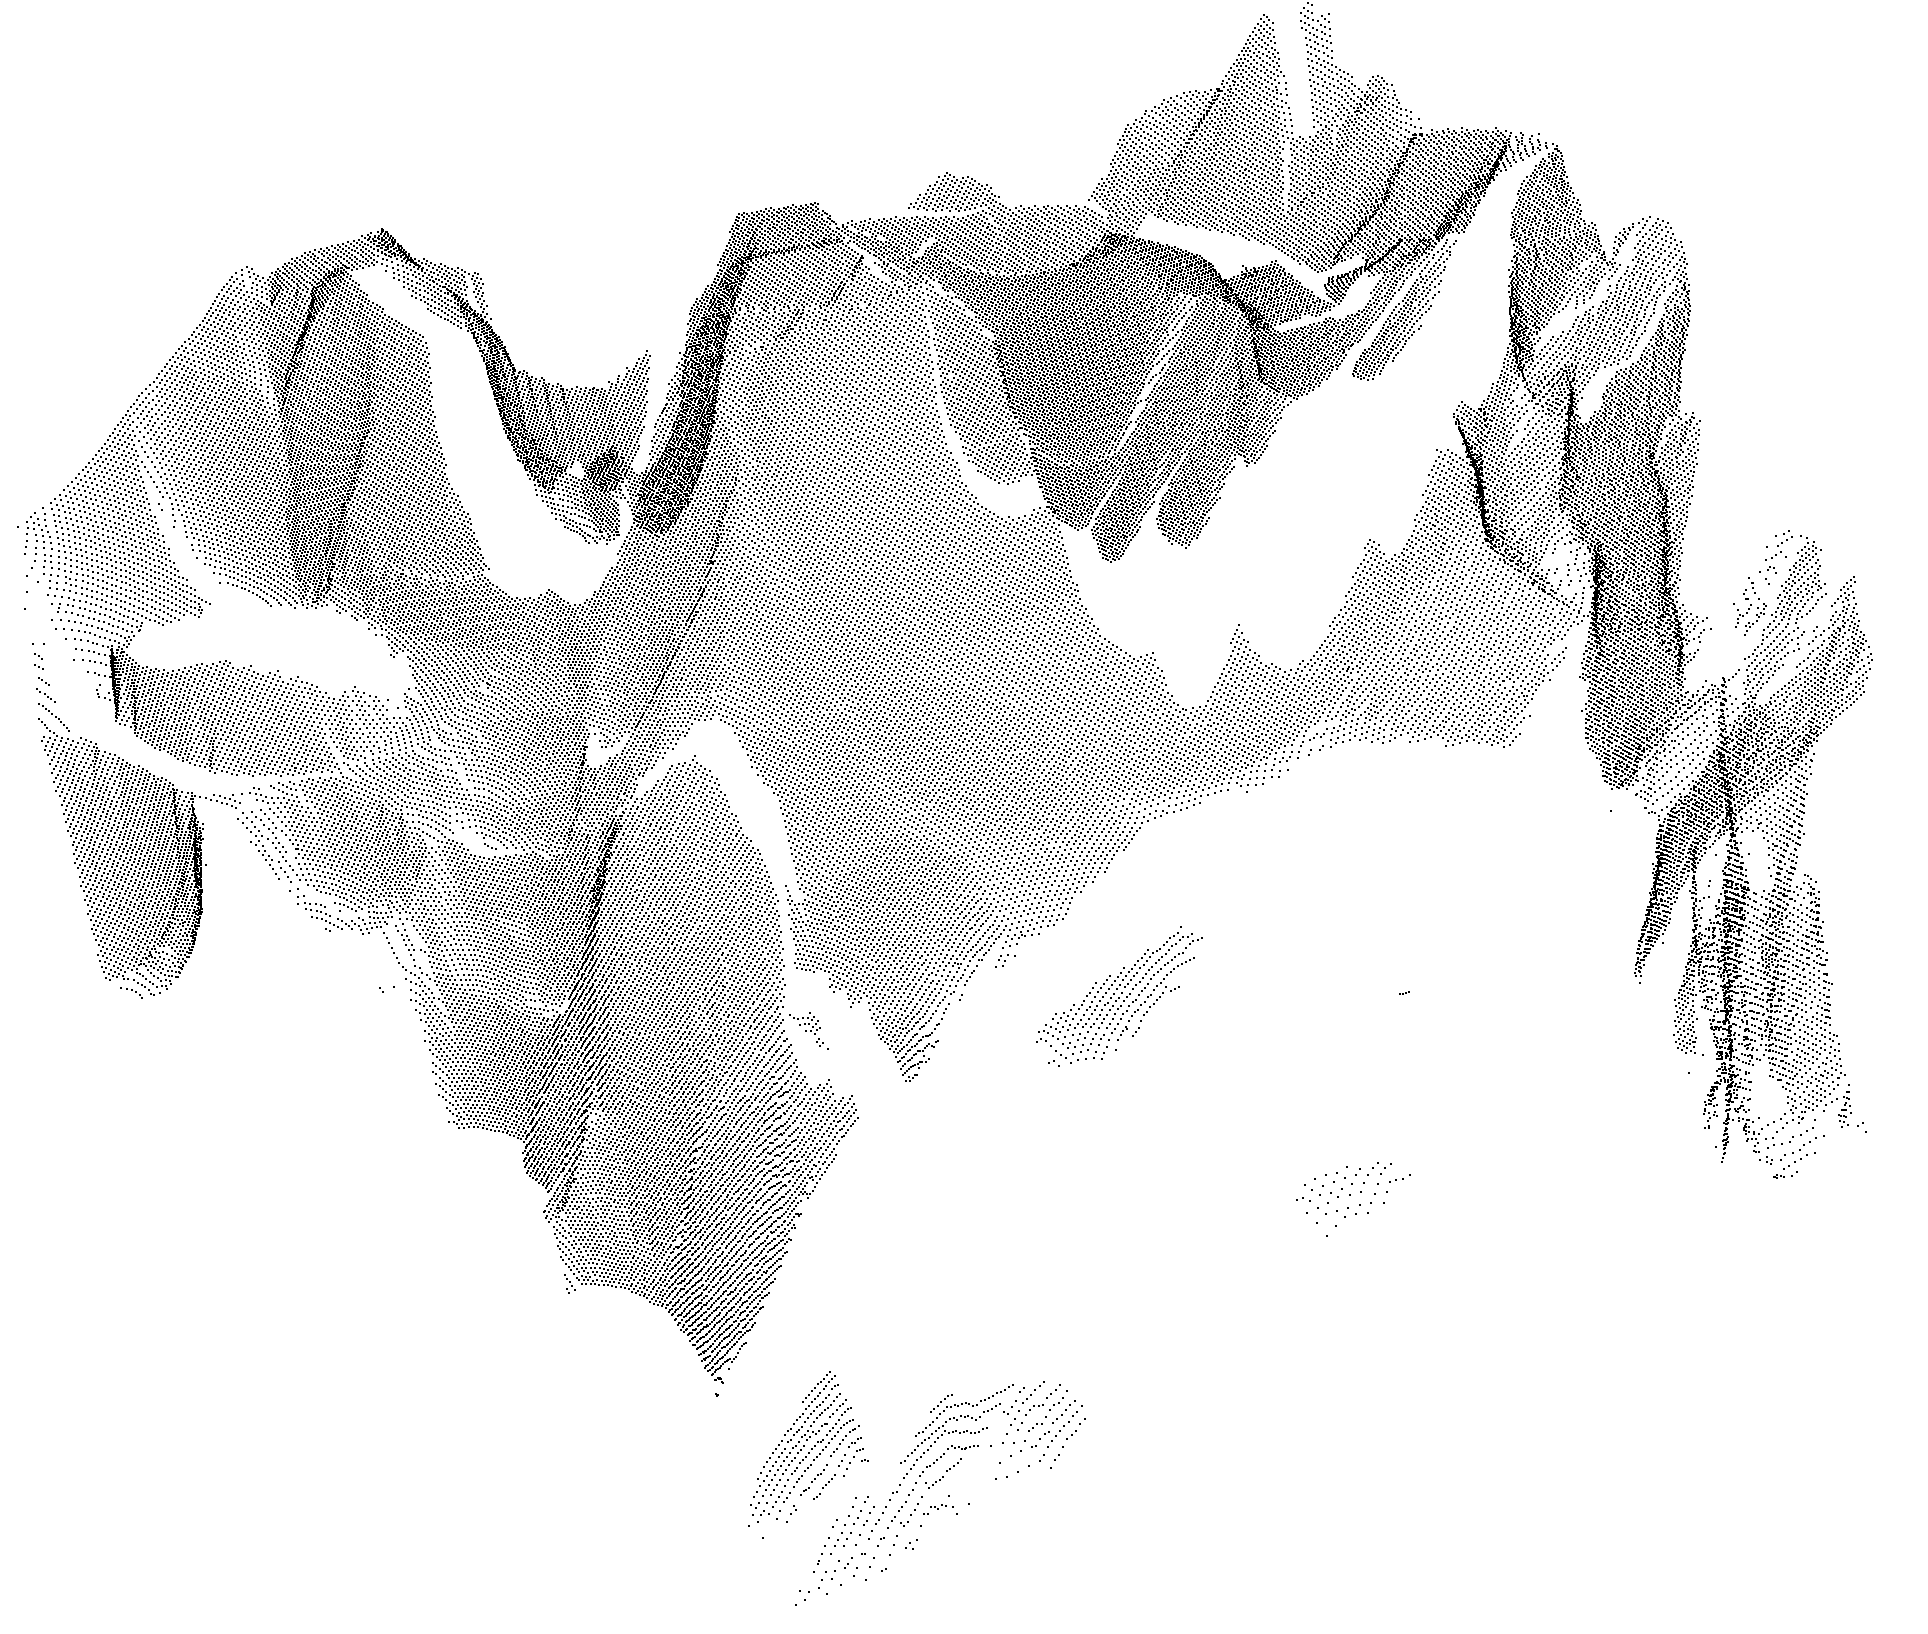
\includegraphics[width=\linewidth]{fig/r1_occlusion2.png}
\end{subfigure}
\caption{Artificial relief surface point cloud with occlusion}
\label{fig:relief_occlusion}
\end{figure}

A triangle mesh is generated by taking points $\{ x, y, R[x,y] \}$ with the $(x,y)$ coordinates forming a square grid of a given density $\rho$, and adding a diagonal edge into each square, in alternating direction. The number of squares per side must be even for this. As can be seen on the renderings in figure \ref{fig:relief_render}, this mesh does not handle the sharp corners well, but it is sufficient as errors are rectified in a later step.

For each triangle, its three vertices are projected into image space, using the given projection camera. This image is a Z-buffer contains, for each pixel, the inverted projected depth of the point\footnote{Z coordinate after application of camera projection matrix.}.

The width and height of this image space is set higher than that of the range image by a factor of about $k = 10$. Now each triangle is filled using a 2D rasterization algorithm. For each pixel, the inverted projected depths of the three corner points are linearly interpolated by using barycentric coordinates. This results in the inverted projected depth of the corresponding 3D surface point.

The actual occlusion culling is now done using a depth test: A pixel value is overwritten only if the inverse depth is higher than the previous one. This is the case only if the point is closer to the camera.

Each $k \times k$ square on this image corresponds to a pixel of the final range image. The center pixel is taken. Given $(x_i, y_i)$ in image space, and the inverse projected depth of the surface point, the 3D coordinates $(x, y, z)$ of the surface points can now be calculated.

Due to the limited accuracy of the mesh, and floating point precision problems, there is some error in this result. It can be rectified by recalculating $z' = R[x, y]$.

\subsubsection{Similarity with actual scans}
Figure \ref{fig:relief_crop} (called $R$) shows an artificial relief point cloud with occluded view and additionally cropped to a random polygonal region inside the original square. It is superimposed on a top-down point cloud of the same relief.

Figure \ref{fig:r1_ddp} (called $D$) is the high-resolution scan of the ``dessus-de-porte'', with colors removed.

The two point clouds are similar these some ways:
\begin{itemize}
\item Approximatively planar. For $R$ the plane is the XY-plane, for $D$ it is the stone surface behind the five statues.
\item Seen from a side angle and partially occluded.
\item Contain both smooth surfaces and sharp corners.
\item Points dispersed on a grid, as a result of the scan-lines, or of the image space in the virtual projection camera.
\end{itemize}

The important difference it that the underlying surface behind $R$ is known. The goal will be to develop a registration method that works for both $R$ and $D$ because of these common characteristics. With $R$ it can be tested both with and without knowledge of the surface.

\begin{figure}[p]
\centering
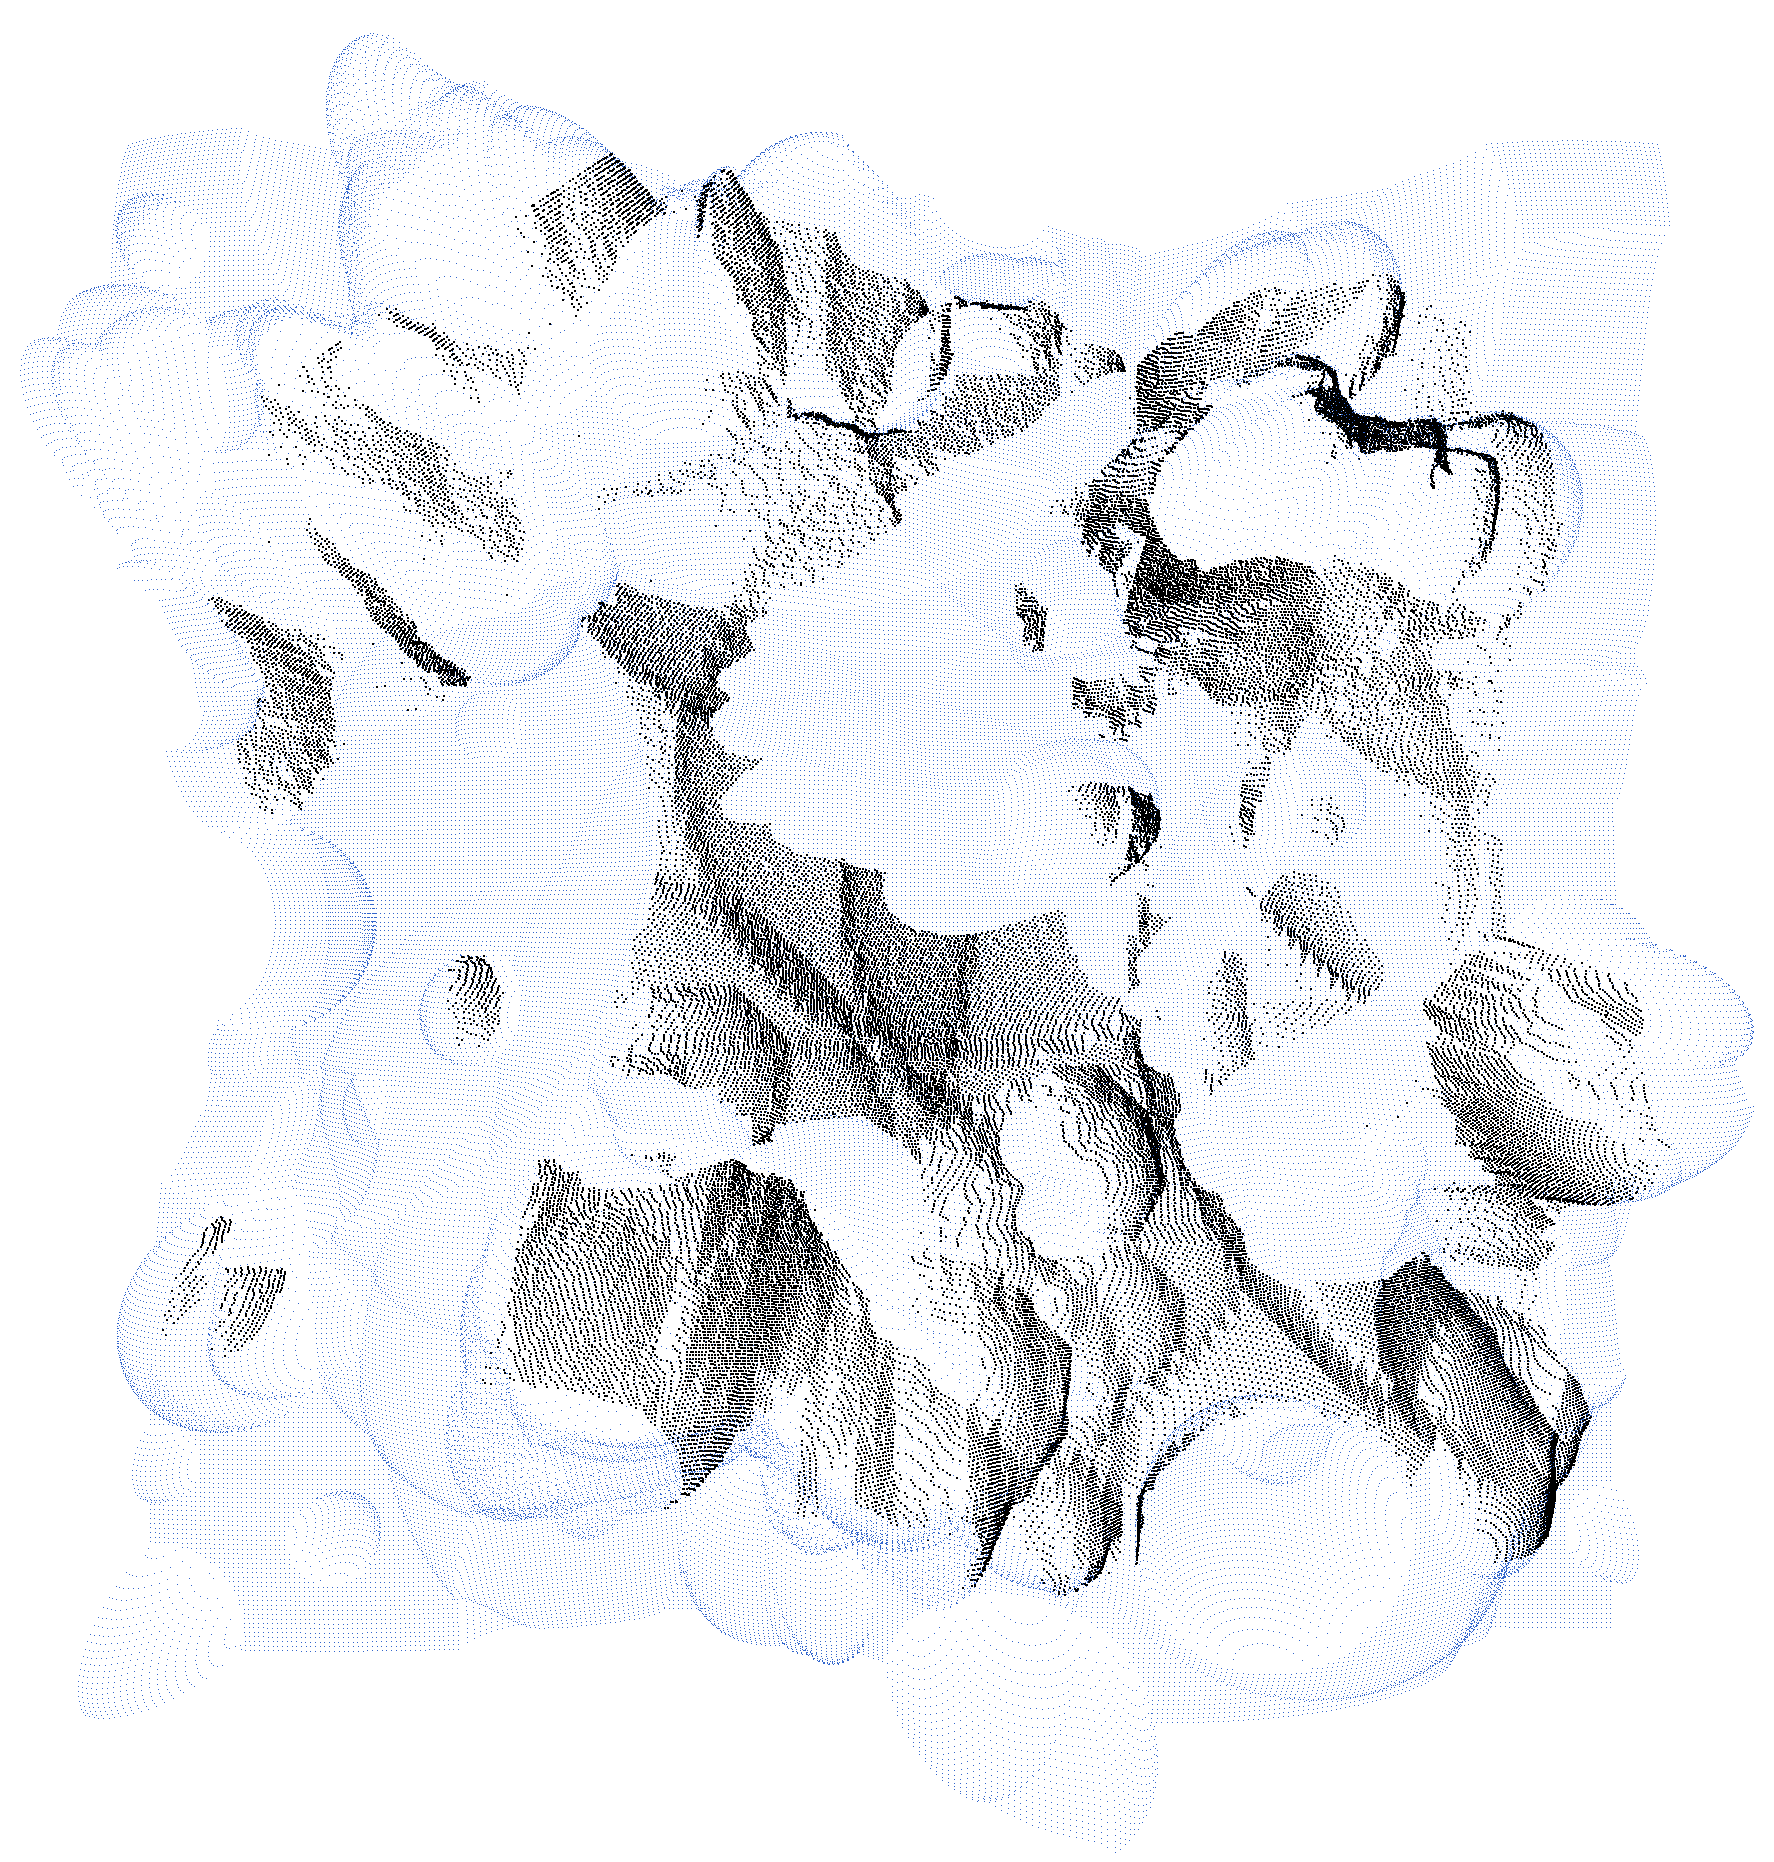
\includegraphics[width=0.7\textwidth]{fig/r1_crop.png}
\caption{$R$: Occluded view point cloud, and top-down point cloud of relief}
\label{fig:relief_crop}
\end{figure}


\begin{figure}[p]
\centering
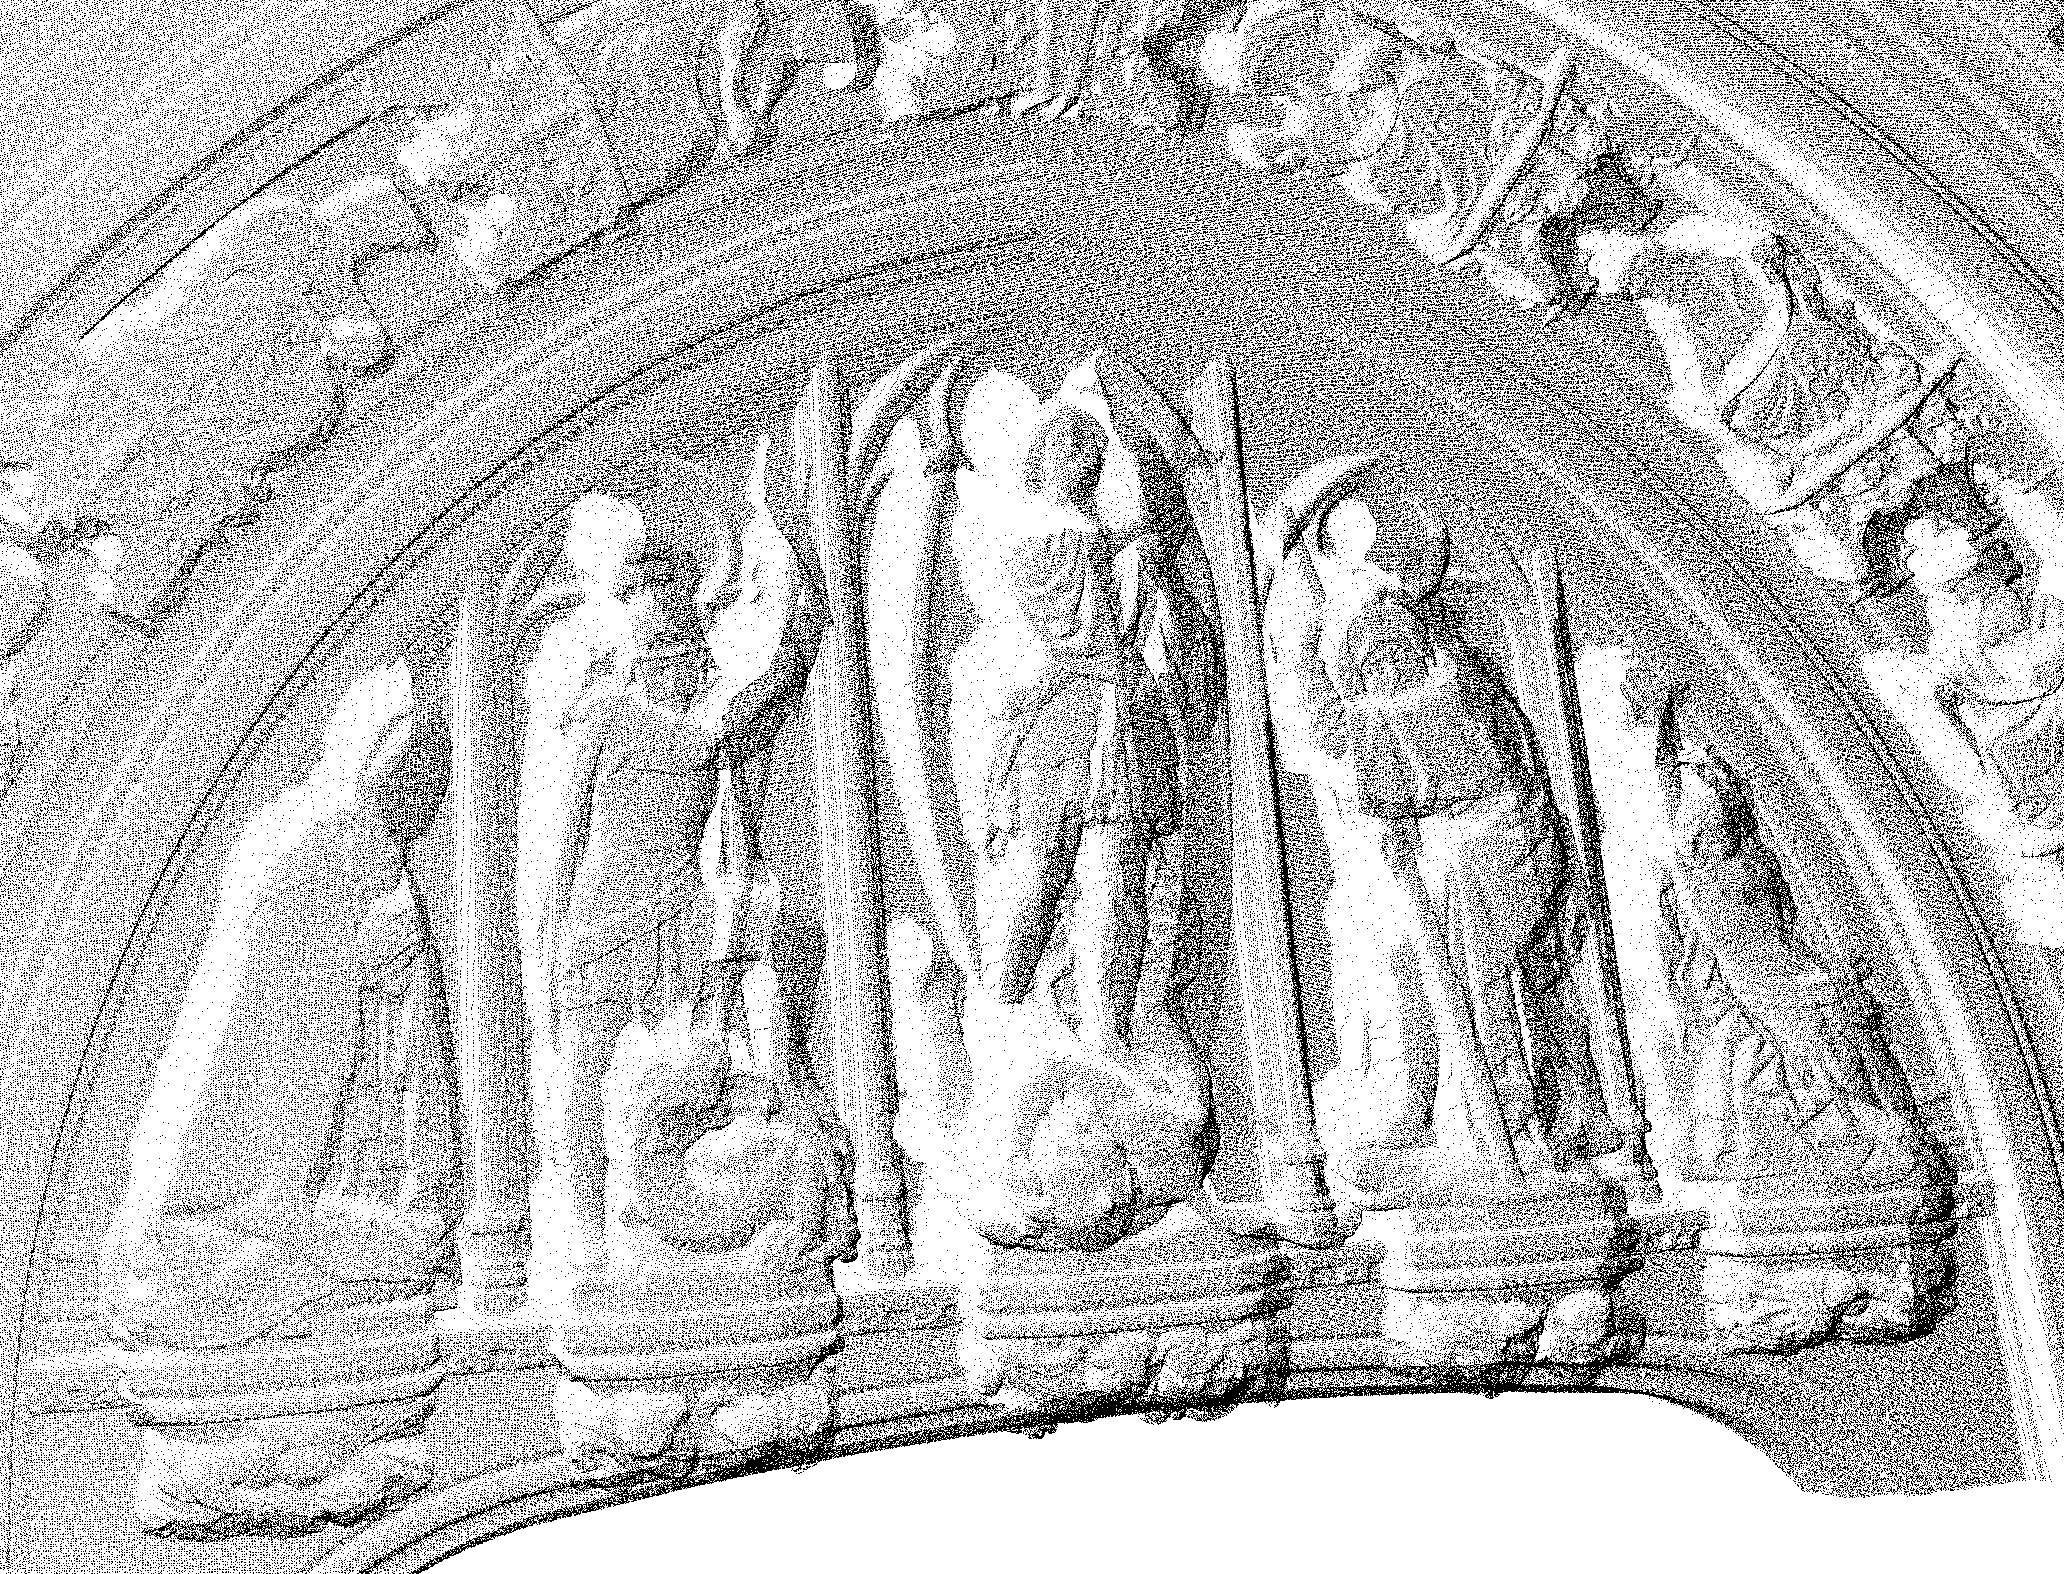
\includegraphics[width=0.7\textwidth]{fig/r1_ddp.png}
\caption{$D$: ``Dessus-de-porte'' point cloud}
\label{fig:r1_ddp}
\end{figure}



\section{Evaluation of registration accuracy}
The output of any registration algorithm that aligns a loose point clouds $Q$ with a fixed point cloud $P$ is a rigid transformation matrix $\matr{\hat{M}}$, or possibly an indication that the algorithm has failed. In the ideal case, which is not reachable in practice, it will be equal to the \emph{true} transformation $\matr{M}$.

In order to evaluate the result, it is useful to have a numerical metric $e(\matr{\hat{M}})$ that indicates the ``accuracy'' of  $\matr{\hat{M}}$, both for the cases when the true transformation is known and when it is unknown. It should be minimal when $\matr{\hat{M}} = \matr{M}$, and it should indicate a spatial distance.



\subsection{Known true transformation} \label{sec:lm_known_ttrans}
When $\matr{M}$ is known, the accuracy is best measured by how much $\matr{\hat{M}}$ deviates from $\matr{M}$. The rigid transformation, relative to the true transformation, is given by $\matr{\hat{M}}_{\text{rel}} = \matr{M} \, \matr{\hat{M}} \, \matr{M}^{-1}$.

Using $\matr{\hat{M}}_{\text{rel}}$, one can calculate for each point $q \in Q$ the \emph{true} correspondence point $q' = \matr{\hat{M}}_{\text{rel}}^{-1} \, \vec{q}$. It is the position in $P$ that corresponds to $q \in Q$. Unless $P$ and $Q$ have the exact same constellation of points, there is generally no point $p \in P$ that coincides with this $q'$. The knowledge of $\matr{M}$ is used to simulate the existence of $P$ with exactly the same constellation.

As a metric for the accuracy of $\matr{\hat{M}}$, the average of the unsigned distances between $q$ and $q'$ is used:
\begin{equation}
e(\matr{\hat{M}}) = \frac{1}{n} \, \sum_{i=1}^{n} \| q - q' \|
\end{equation}
This value will be called the \emph{true error}. It is similar to the ICP point-to-point error metric, just with the real correspondences, and without squaring the terms. Using a point-to-plane or other metric would not be useful because the correspondences are exact.

When $\matr{\hat{M}} = \matr{M}$, the absolute minimum $e(\matr{\hat{M}}) = 0$ is reached, as all points $q = q'$ coincide. When $\matr{M}$ is only a translation $\vec{t}$, $e(\matr{\hat{M}}) = \| \vec{t} \|$. When a small rotation with center $\vec{0}$ (the origin $Q$) is added, all points $q$ move away from $q'$ in a circular motion. Using trigonometric approximation for small angles, this length of movement is proportional to $\| q, \vec{0 }\|$ (and not to the squared distance). Hence taking the average of unsigned distances $q - q'$ can give a useful value.


\subsection{Unknown true transformation}
When $\matr{M}$ is unknown, no exact metric for the accuracy can be defined. As with ICP, the correspondences can be approximated using the closest point criterion or a variation of it. However, here the point clouds are not assumed to be in the process of converging towards an alignment, but rather the goal is to evaluate the accuracy of a finished alignment, or to tell whether the registration has led to a local minimum.

The point-to-point or other error metrics used by ICP depend on the estimated point correspondences, and attain local minima for values of $\matr{M}$ where the estimated correspondences are incorrect, but have low average distances. Also the correspondence selection needs to be adjusted in function of the occlusions, different bounds and densities of $P$ and $Q$. 

An error metric calculated from one-on-one point correspondences is necessarily limited by the which points are available in $P$ and $Q$. Techniques such as point-to-plane ICP and generalized ICP try to infer information about the local shape of the surface around a point.

In this chapter, an attempt will be made to define a fine registration accuracy measure, based on the histogram formed by the distances of point pairs chosen using the closest point criterion. For this the dispersion of points on the surfaces will be taken into account. 


\section{Analysis of point clouds}
In this section the points of the point clouds are looked at in more detail, including their dispersion pattern on the surfaces.

\subsection{Local measures}
Some local measures will be defined that assign to each point in the point cloud a value in relation with its surrounding points. They will be used in the following development.

\subsubsection{Estimated density}
The \emph{local surface density} $\rho(p)$ of a point cloud $P$ around a point $p \in P$ indicates how densely points are dispersed on the surface around $p$, expressed in number of points per surface area. Because the shape of the underlying surface is unknown, a precise measure cannot be defined, and instead an approximation is used.

Taking the $k$ nearest neighbors around a point $p$ that is in a region where the surface is approximately planar results in a set of points located approximately on a disk around $p$. In this case, an estimate for the density is $\rho(p) = \frac{k}{\pi \, r_{\text{max}}^2}$, where $r_{\text{max}}$ is the maximal distance of one of the neighbors to $p$.

Even when the surface is not locally planar in that region, some level of accuracy is retained because Euclidian distances in three-dimensional space are measured, which are approximatively equal to arc distances along the surface on which the disk would be wrapped.

Using $r_{\text{max}}$ makes the measure more sensitive to outliers, and can overestimate the density: $r_{\text{max}}$ by definition is the smallest least radius such that $k$ points are inside the disk. An alternative is to use the median $r_{\text{med}}$ of the radii, and set $\rho(p) = \frac{k}{2 \, \pi \, r_{\text{med}}^2}$. For the median value, half of the $k$ points have a smaller radius and are thus inside the disk.

When the density is supposed to be constant for each point in the point cloud, it will also be denoted as $\rho$ or $\rho(P)$.

\subsubsection{Square grid density}
For artificially generated point clouds, per-point densities $\rho(p)$ are set to their theoretical values. For a planar surface where points are arranged on a square grid with side length $l$, this density is $\rho(p) = \frac{1}{l^2}$, because $1$ point can be counted per square. This will be extended to parallelogram grids in the next section.


\subsubsection{Curvature}
In the rest of this chapter, properties of the dispersion of points on planar surfaces of the model will be used. It is therefore important to distinguish between approximatively planar regions of the surface, and more sharp edges.

Unlike the density, this is a measure of the surface and not of the point dispersion on it. This implies that the metric should be invariant of the point dispersion. In addition to this, it is dependent on a scale parameter: for example a point cloud representing a wall of a building would be planar on a scale of a few centimeters, but not on a millimeter scale where the texture of the wall is considered.

A measure of \emph{local curvature} $c(p, r)$ around a point $p \in P$ with a radius $r \in \mathbb{R}$ will be defined. A tangent plane is attached to the point $p$, with the same normal vector $\vec{n}$ as the point. This normal vector is assumed to have been calculated beforehand, for example by least-squares of RANSAC plane fitting. Then it is measured how well the neighboring points fit on the plane.

Using the local density $\rho(p)$, the expected number of points located in a radius $r$ on the surface is $\rho(p) \, \pi \, r^2$. Using a kNN algorithm the $k = \lceil \rho(p) \, \pi \, r^2 \rceil$ nearest neighbors $N_k \subset P$ are searched. When $k$ is below a predefined threshold it is increased to a minimal value. 

If the surface is locally planar around and $p$ in the given radius, the points $N_k$ will be located in a disk around $p$, with a radius of approximatively $r$. Because the circumference of a circle is proportional to its radius, $N_k$ contains more points at higher radii, and the probability density of their distance to $p$ increases linearly. But these points at a higher distance that fit on the plane should not overcompensate for nearer points that don't. Weights are attributed to the points to cancel out that effect: The weight of the closest point $p_1$ is set to $1$, and those of the remaining points $p_i$ to $\frac{\| p_1 - p \|}{\| p_i - p \|}$. Then the weights are normalized to sum up to $1$.

To measure how well a point $p_i \in N_k$ fits the plane, two values are useful: Its distance $d_i$ to the plane, and the absolute angle $|\alpha_i|$ between its normal vector and that of the plane. Both can be calculated using the dot products:
\begin{equation}
d_i = \vec{n} \, (\vec{p_i} - \vec{p})
\hspace{7mm} \text{and} \hspace{7mm}
\cos \alpha_i = \vec{n} \, \vec{n_i}
\end{equation}

The local curvature metric is calculated as weighted average of those values for the $k$ neighboring points:
\begin{equation}
c(p, r) = \sum_{i=1}^{k} w_i \, \left( A \, |\alpha_i| + D \, d_i \right)
\end{equation}
where the coefficients $A$ and $D$ are set so as to attribute different weights to the two measures. To avoid evaluating $\arccos$ for each point, the angle can be approximated using $\alpha'_i = \frac{\pi}{2} (1 - \vec{n} \, \vec{n_i})$. These two figures show two surfaces in one dimension where one metric it high and the other low.
\begin{figure}[H]
\centering
\begin{subfigure}{.4\textwidth}
	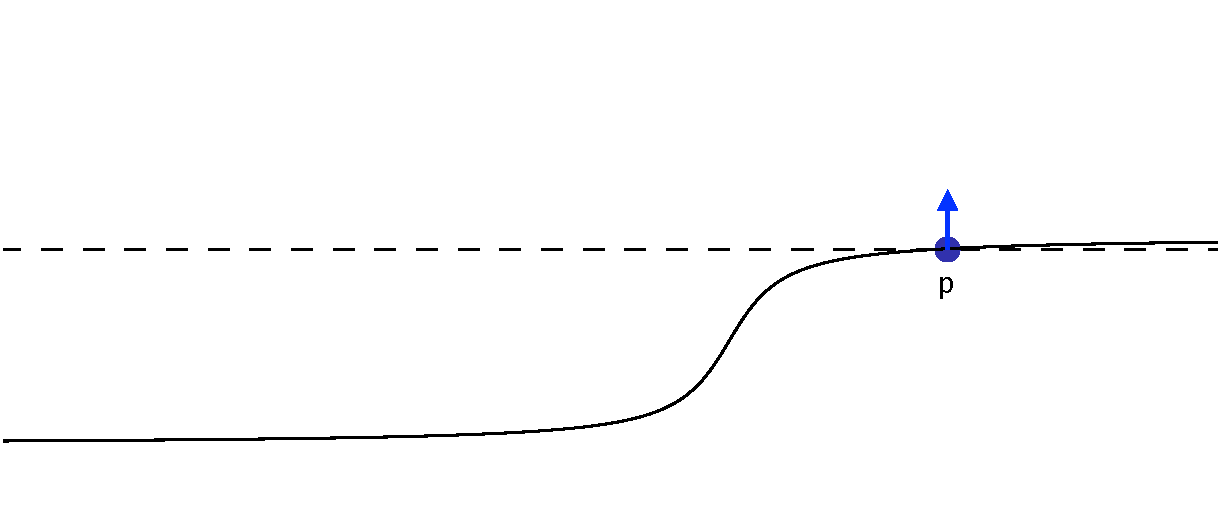
\includegraphics[width=\linewidth]{fig/curvature_distances.pdf}
	\caption{Large $\sum d_i$, small $\sum |\alpha_i|$}
\end{subfigure}%
\hspace{15mm}%
\begin{subfigure}{.4\textwidth}
	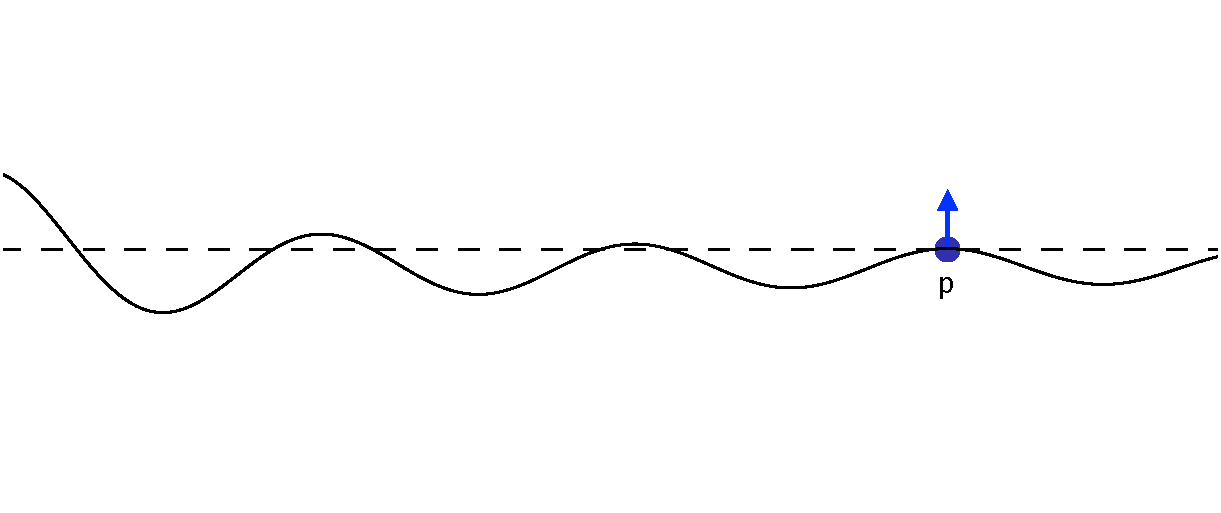
\includegraphics[width=\linewidth]{fig/curvature_angles.pdf}
	\caption{Large $\sum |\alpha_i|$, small $\sum d_i$}
\end{subfigure}	
\end{figure}
For the purposes that the curvature measure is used here, $A$ should be set higher, because surfaces such as the left-side can still be considered to be locally planar.






\subsection{Point dispersion}
Point dispersion refers to how points in a point clouds are arranged on a surface. When the surface is locally planar, regions of the surface can be approximated by a plane. The following three point dispersions on the plane will be analyzed:
\begin{figure}[H]
\centering
\hspace*{\fill}%
\begin{subfigure}{.3\textwidth}
{
	\setlength{\fboxsep}{0pt}%
	\setlength{\fboxrule}{0.5pt}%
	\fbox{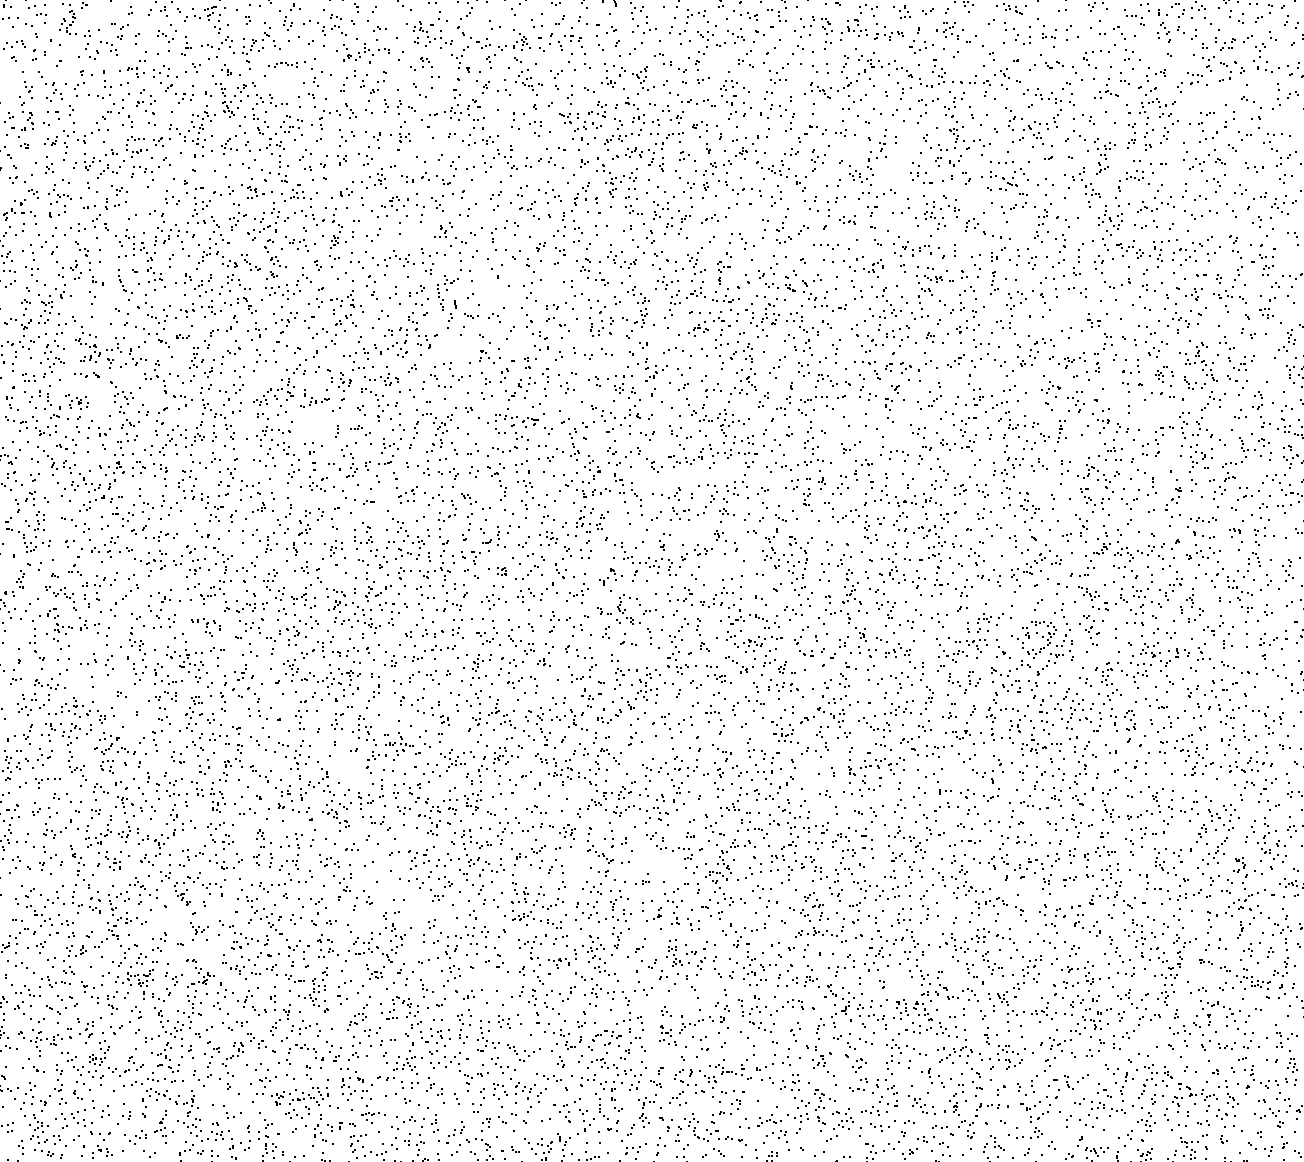
\includegraphics[width=\linewidth]{fig/dispersion_random.png}}%
	\caption{Random dispersion}
}
\end{subfigure}%
\hfill%
\begin{subfigure}{.3\textwidth}
{
	\setlength{\fboxsep}{0pt}%
	\setlength{\fboxrule}{0.5pt}%
	\fbox{
\includegraphics[width=\linewidth]{fig/dispersion_sqgrid.png}}%
	\caption{Square grid}
}
\end{subfigure}%
\hfill%
\begin{subfigure}{.3\textwidth}
{
	\setlength{\fboxsep}{0pt}%
	\setlength{\fboxrule}{0.5pt}%
	\fbox{
\includegraphics[width=\linewidth]{fig/dispersion_pargrid.png}}%
	\caption{Parallelogram grid}
}%
\end{subfigure}\\
\caption{Different point dispersions on planar surface}
\label{fig:point_dispersion}
\end{figure}

The \emph{random dispersion} is the most general case, where the $x$ and $y$ coordinates of each points are independent, random variables, with a uniform distribution. It can be seen visually that the local density in that case is not constant.

Point clouds recorded by a laser scanner will produce a dispersion that is more akin to the \emph{square grid dispersion}. If the scanner processes in sequential scan-lines, and uses a regular graduation of azimuth and elevation coordinates, a planar surface placed perpendicular to the scanner ray will \emph{locally} get points approximatively arranged in squares. The dispersion will be considered to be invariant to a two-dimensional rotation of the plane itself.

\subsection{Parallelogram grid}
When the surface is placed at an oblique angle to the scanner line, the points on the plane will instead be dispersed on a \emph{parallelogram grid}. Figures \ref{fig:closeup_ddp}, \ref{fig:closeup_wall} show two close-up views of the ``Hôtel de Ville'' scans, featuring the parallelogram grid point dispersion on approximatively planar surfaces. Figure \ref{fig:bunny_grid_closeup} is taken from the Stanford Bunny point cloud, which was also recorded using a laser scanner. The square grid or rectangular grid are special case of this.

\begin{figure}[p]
\centering
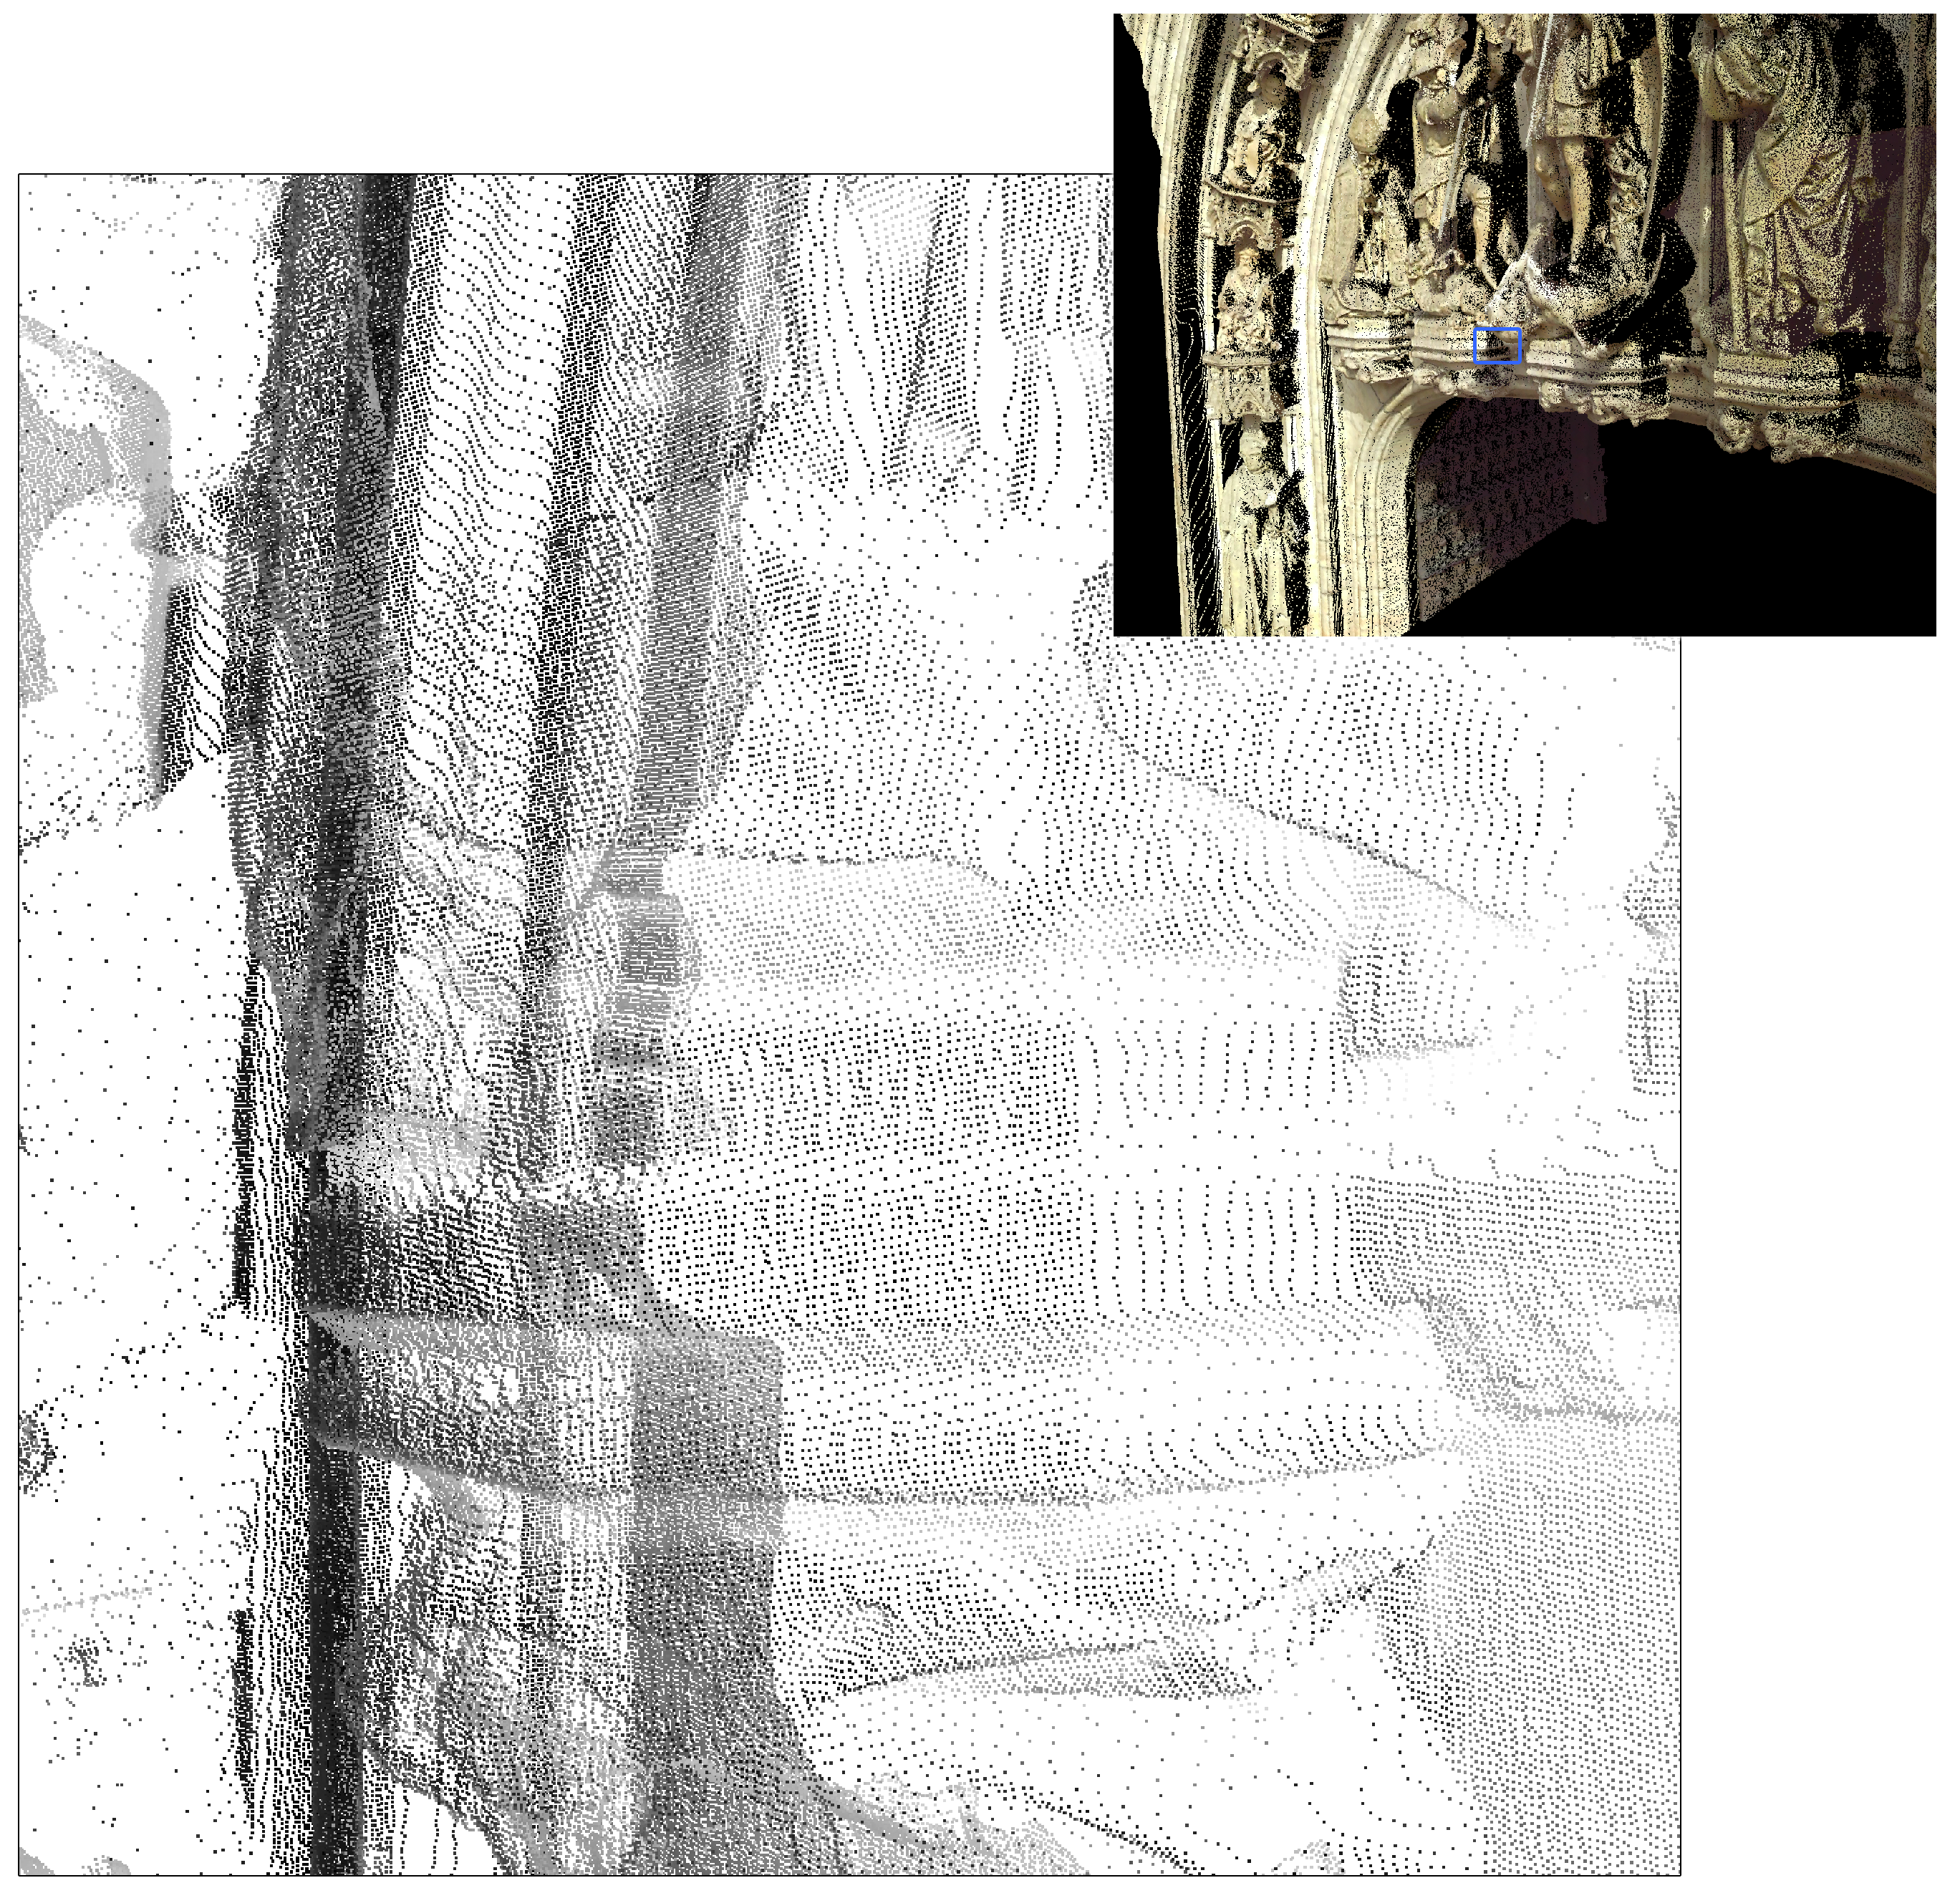
\includegraphics[width=.6\textwidth]{fig/closeup_ddp.png}
\caption{Closeup of the surface distribution of points on front wall of building}
\label{fig:closeup_ddp}
\end{figure}

\begin{figure}[p]
\centering
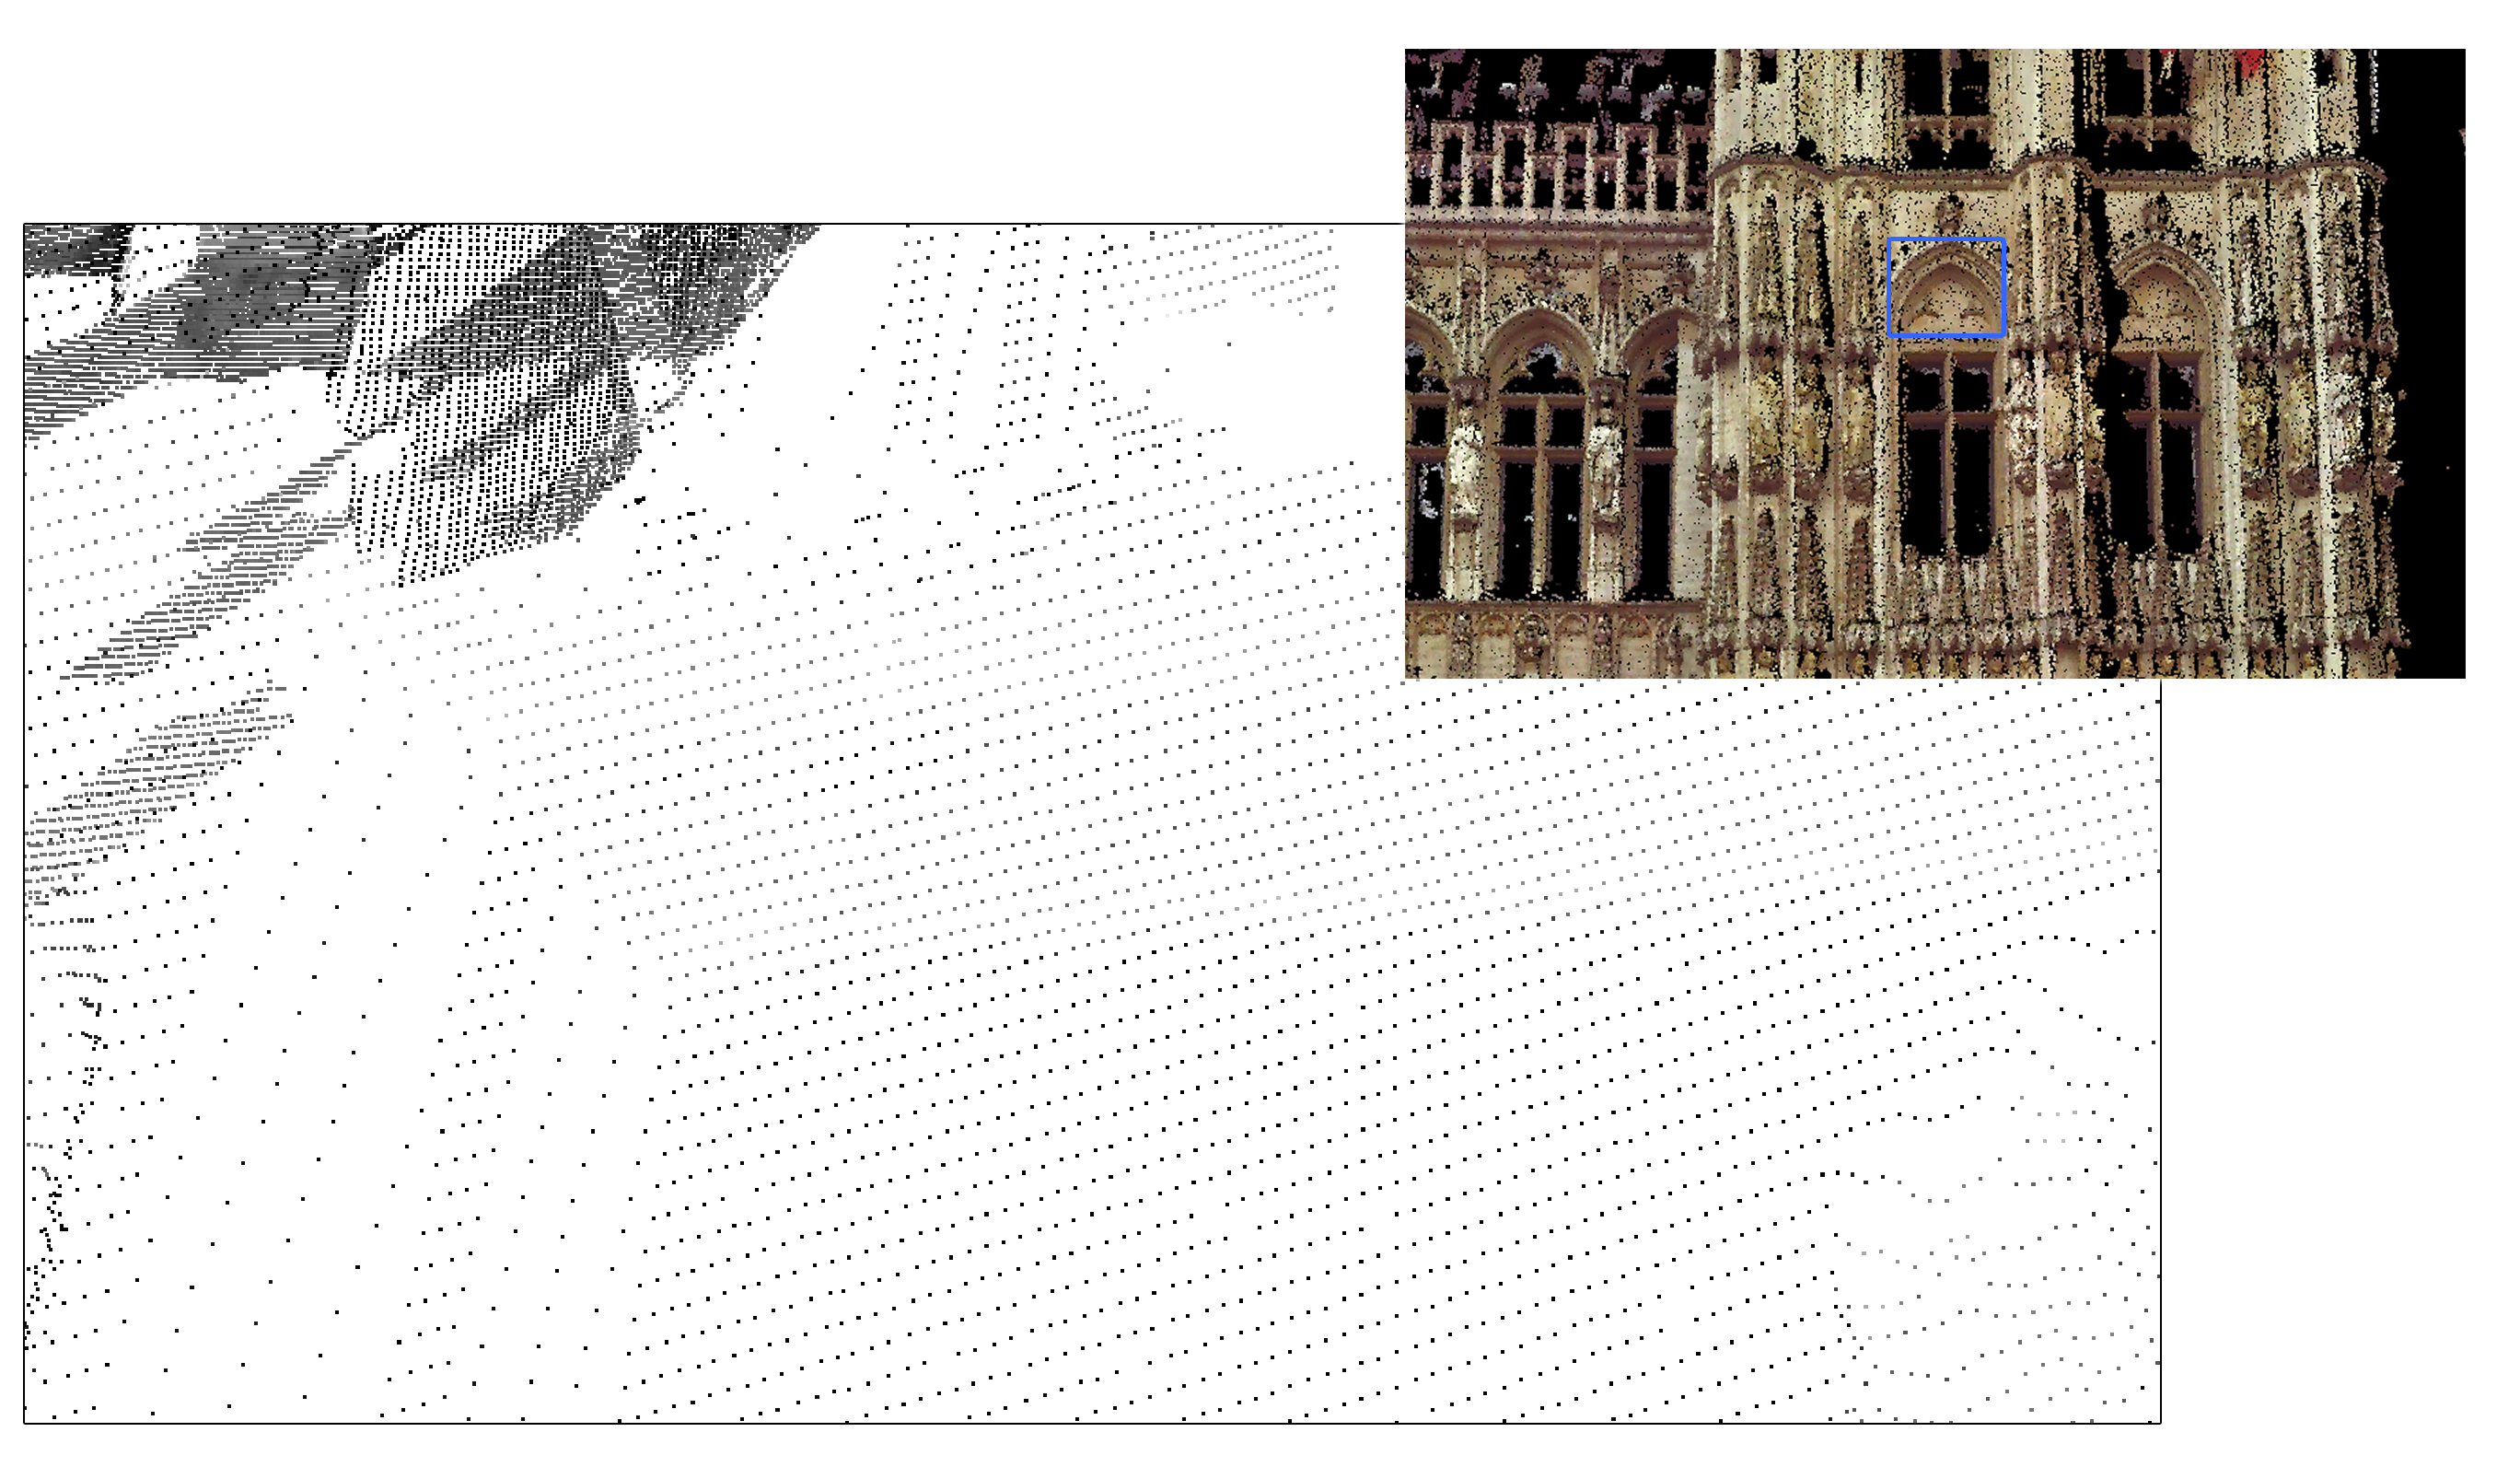
\includegraphics[width=.6\textwidth]{fig/closeup_wall.png}
\caption{Closeup of the surface distribution of points on detail of ``dessus-de-porte''}
\label{fig:closeup_wall}
\end{figure}

\begin{figure}[p]
\centering
{
	\setlength{\fboxsep}{0pt}%
	\setlength{\fboxrule}{0.5pt}%
	\fbox{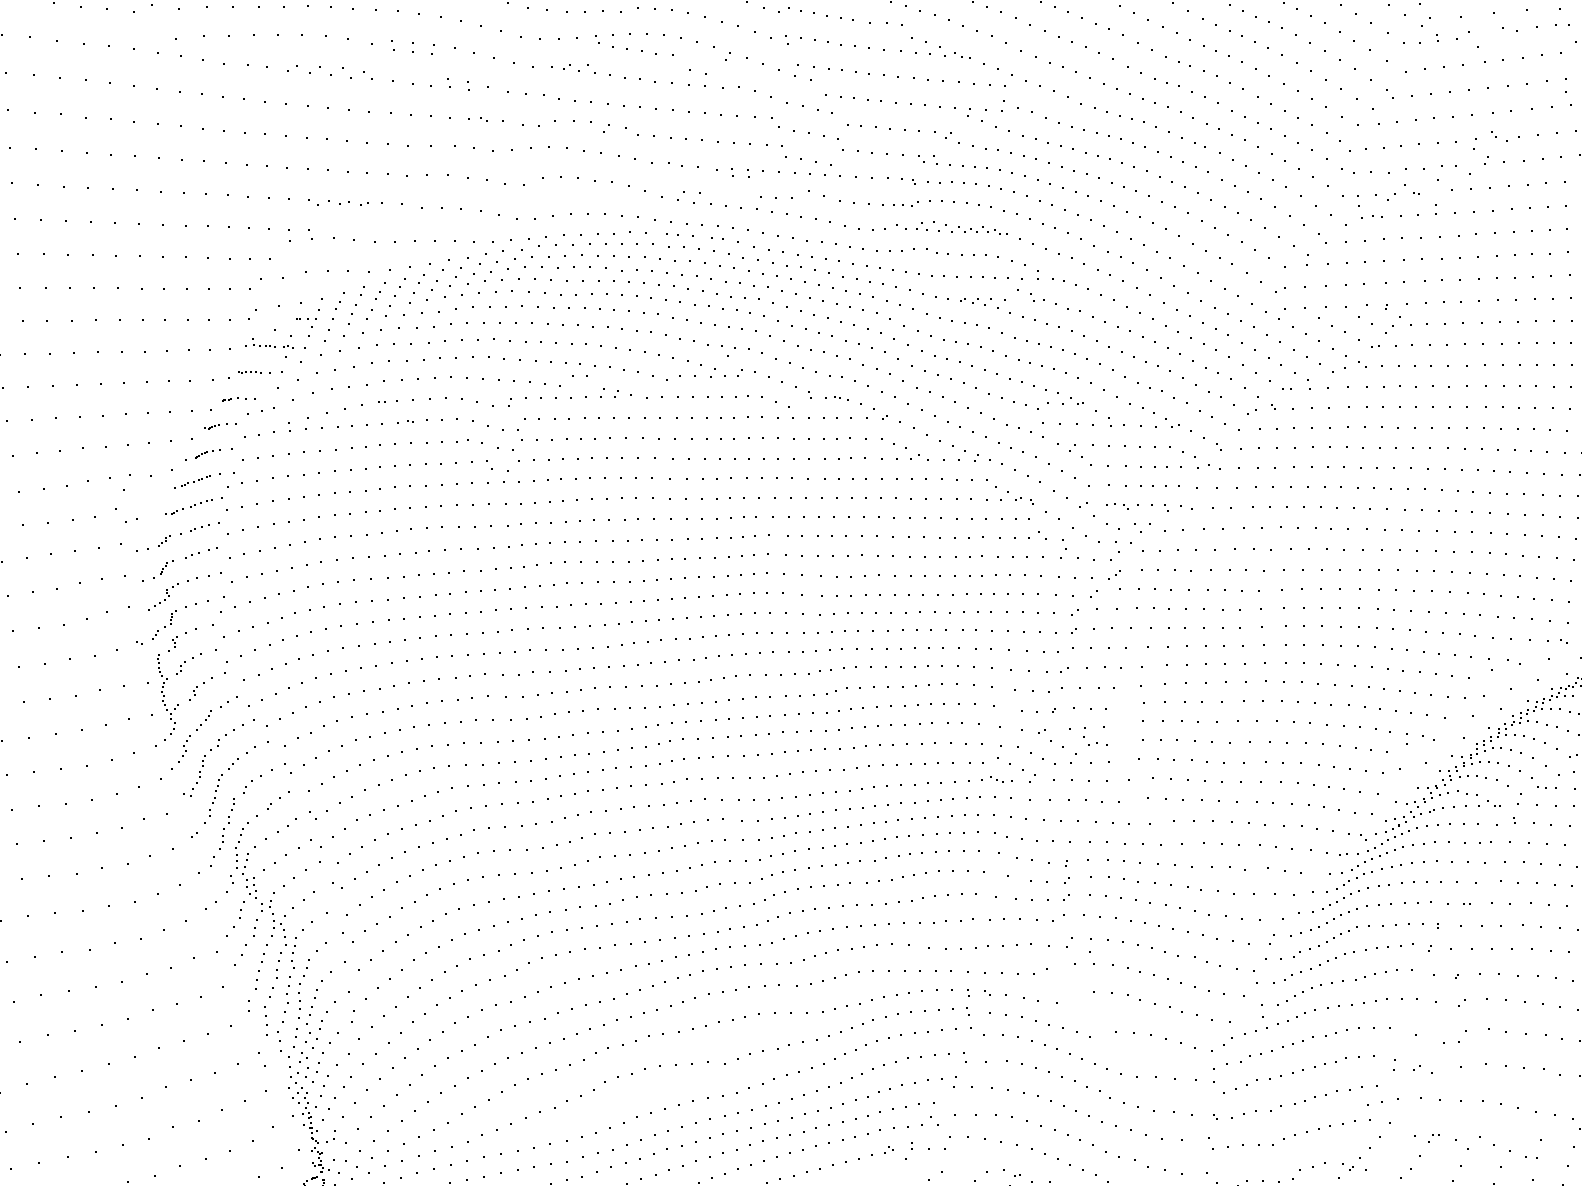
\includegraphics[width=.4\textwidth]{fig/bunny_grid_closeup.png}}
}
\caption{Closeup of the surface distribution of points on Bunny point cloud}
\label{fig:bunny_grid_closeup}
\end{figure}

The diagram on figure \ref{fig:pargrid_proj} shows the parallel projection of a square from camera image space onto a plane in three-dimensional space. $\vec{n}$ is the normal vector of the plane, $p_l$ the width and height (side length) of the square, and $x, y$ the corresponding side lengths of the projected square. It can be seen that the projected square takes on the shape of a parallelogram on the plane. This models the projection of scanner rays on a surface. The coordinate system is such that the scanner is placed at origin. Since only a small region of a locally planar surface is considered (compared to the field of view of the scanner), adjacent rays in azimuth and elevation direction are modeled as parallel. When the square is extended to form a square grid in the XY-plane, a parallelogram grid is formed on the plane in which all parallelograms have the same two side lengths and inner angles.

\begin{figure}[h]
\centering
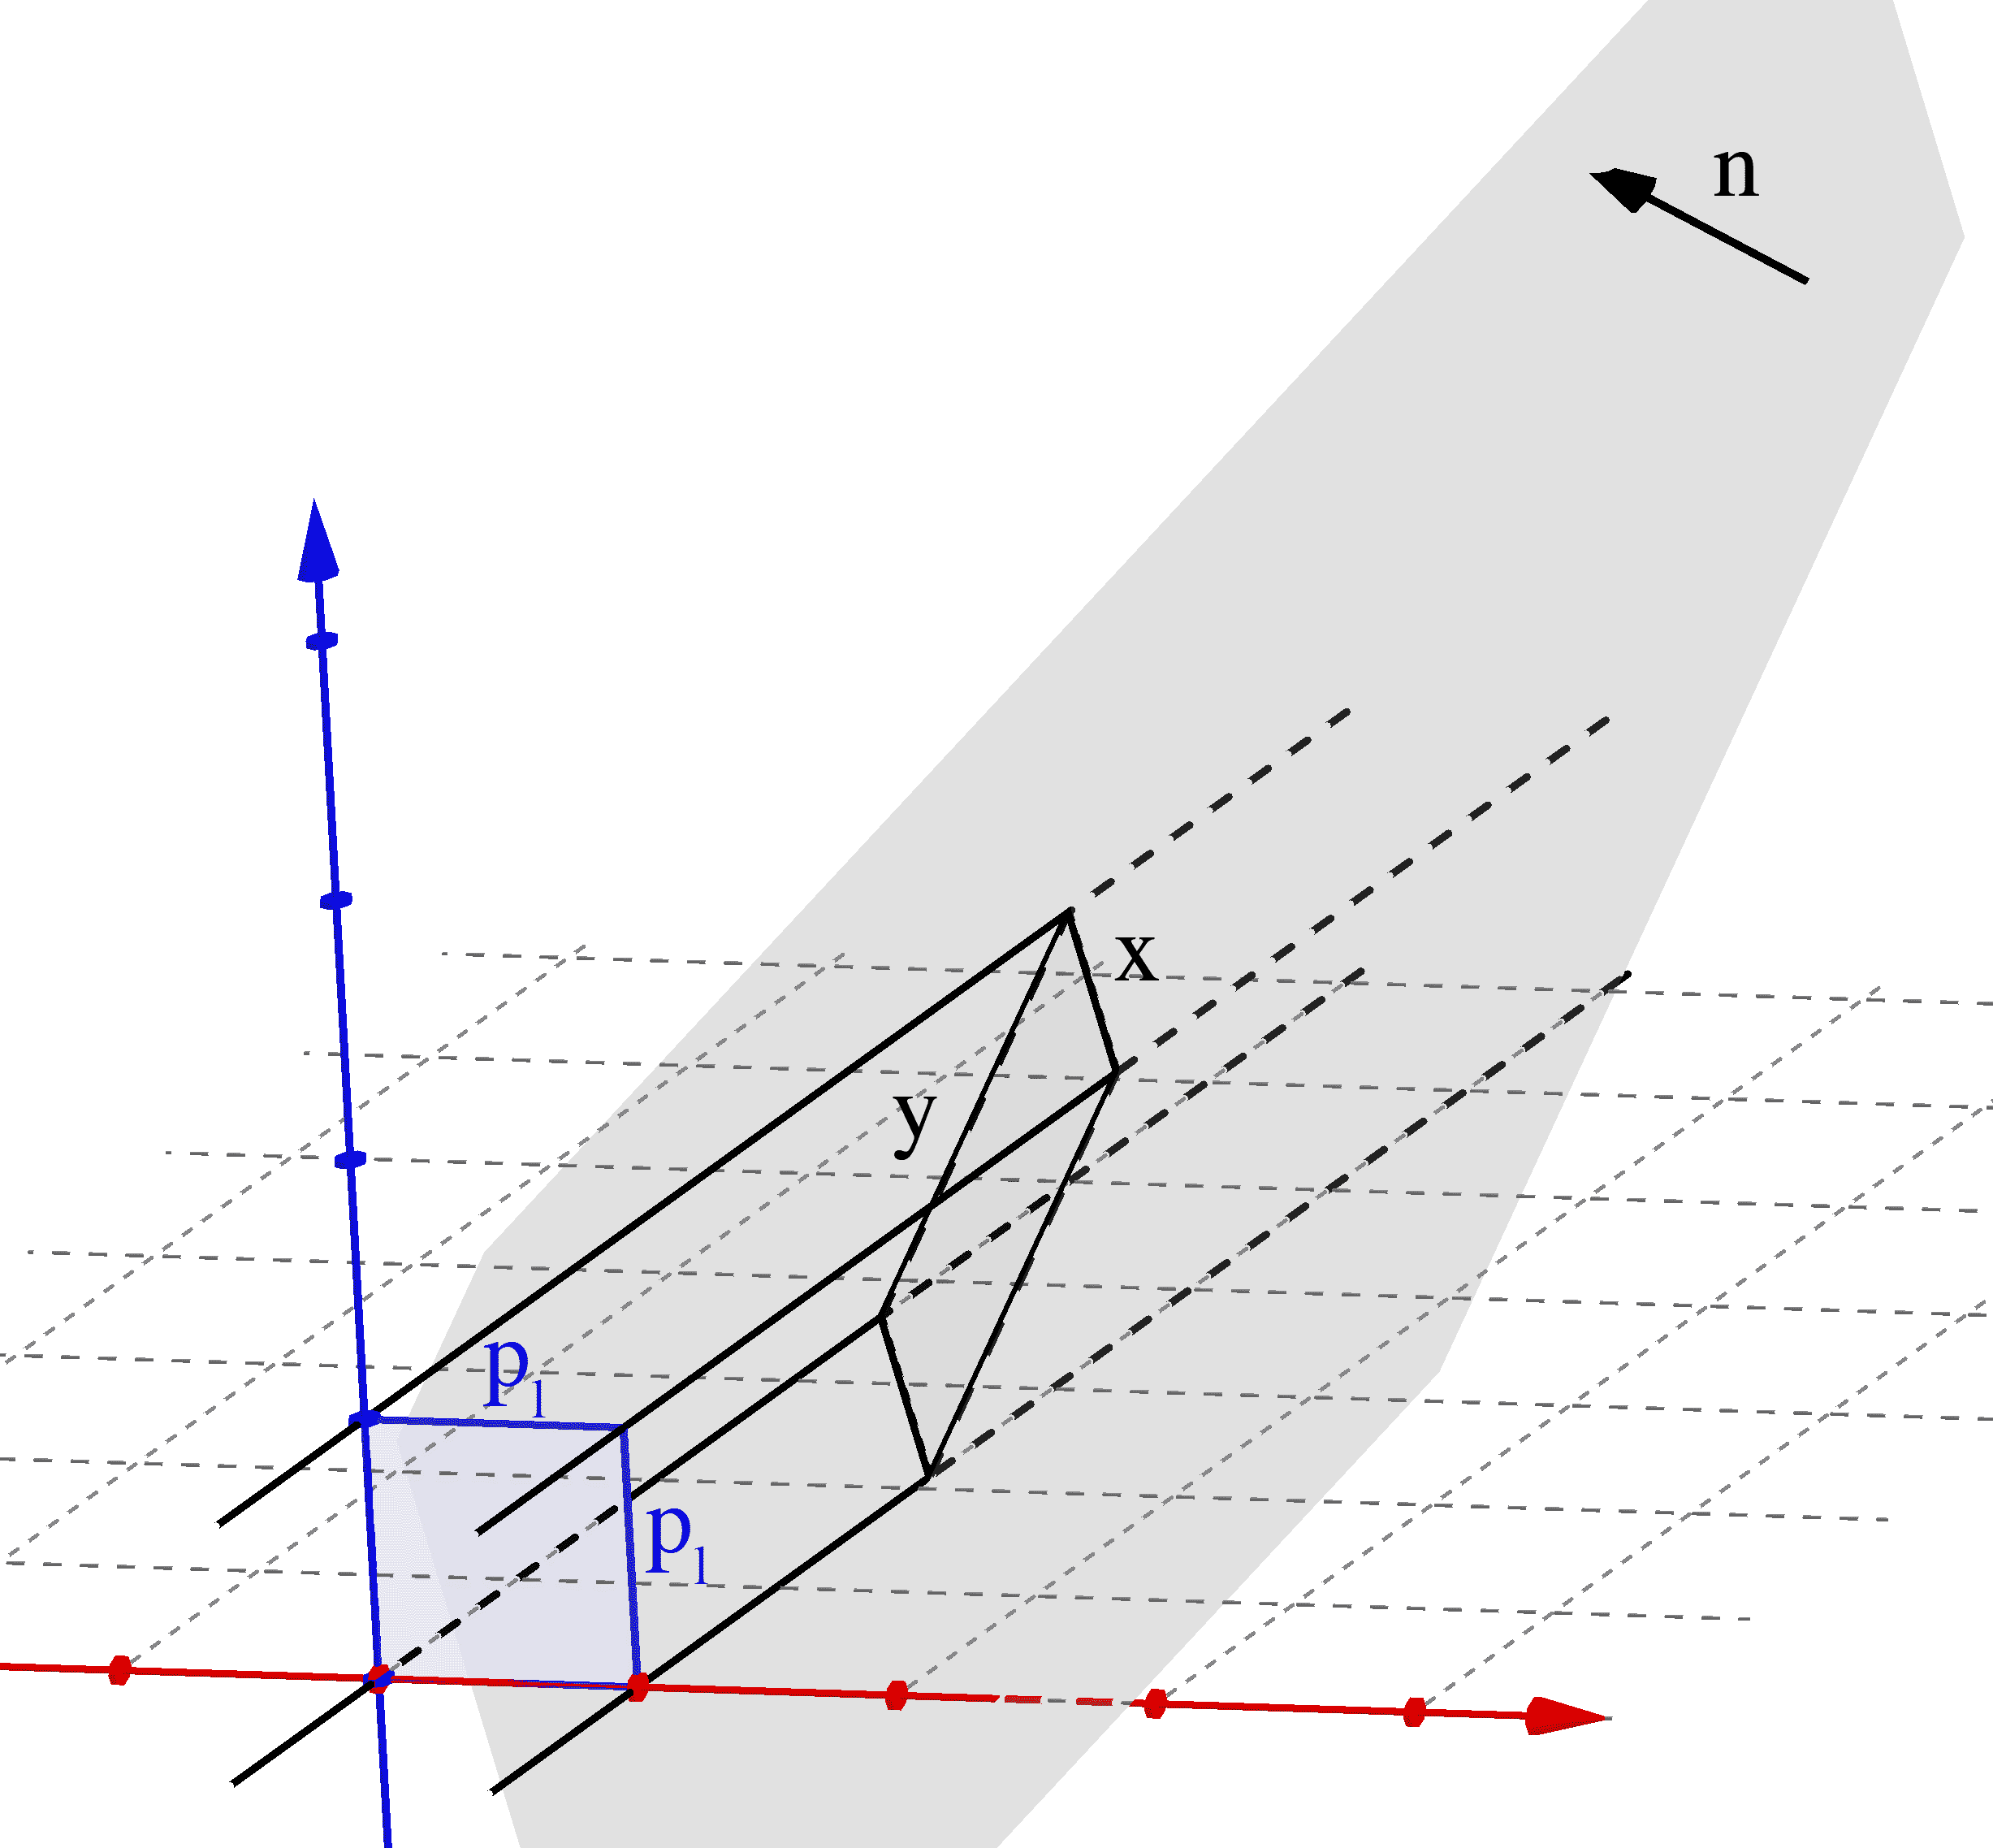
\includegraphics[width=.4\textwidth]{fig/pargrid_proj.png}
\caption{Parallel projection of square onto plane in space}
\label{fig:pargrid_proj}
\end{figure}

It can be seen on figure \ref{fig:par_grid_tilings} that several different parallelogram grids are possible for the same dispersion of points on the plane. The two grids in these examples have no sides in common. The projection of the camera square grid on the plane results in one of the possible parallel grids. When the plane is placed at a more oblique angle from the camera, it tends to be a grid with longer side lengths, such as the second on on the figure. It is not necessarily such that it includes the shortest possible parallelogram edge.

\begin{figure}[h]
\centering
\hspace*{\fill}%
\begin{subfigure}{.33\textwidth}
{
	\setlength{\fboxsep}{0pt}%
	\setlength{\fboxrule}{0.5pt}%
	\fbox{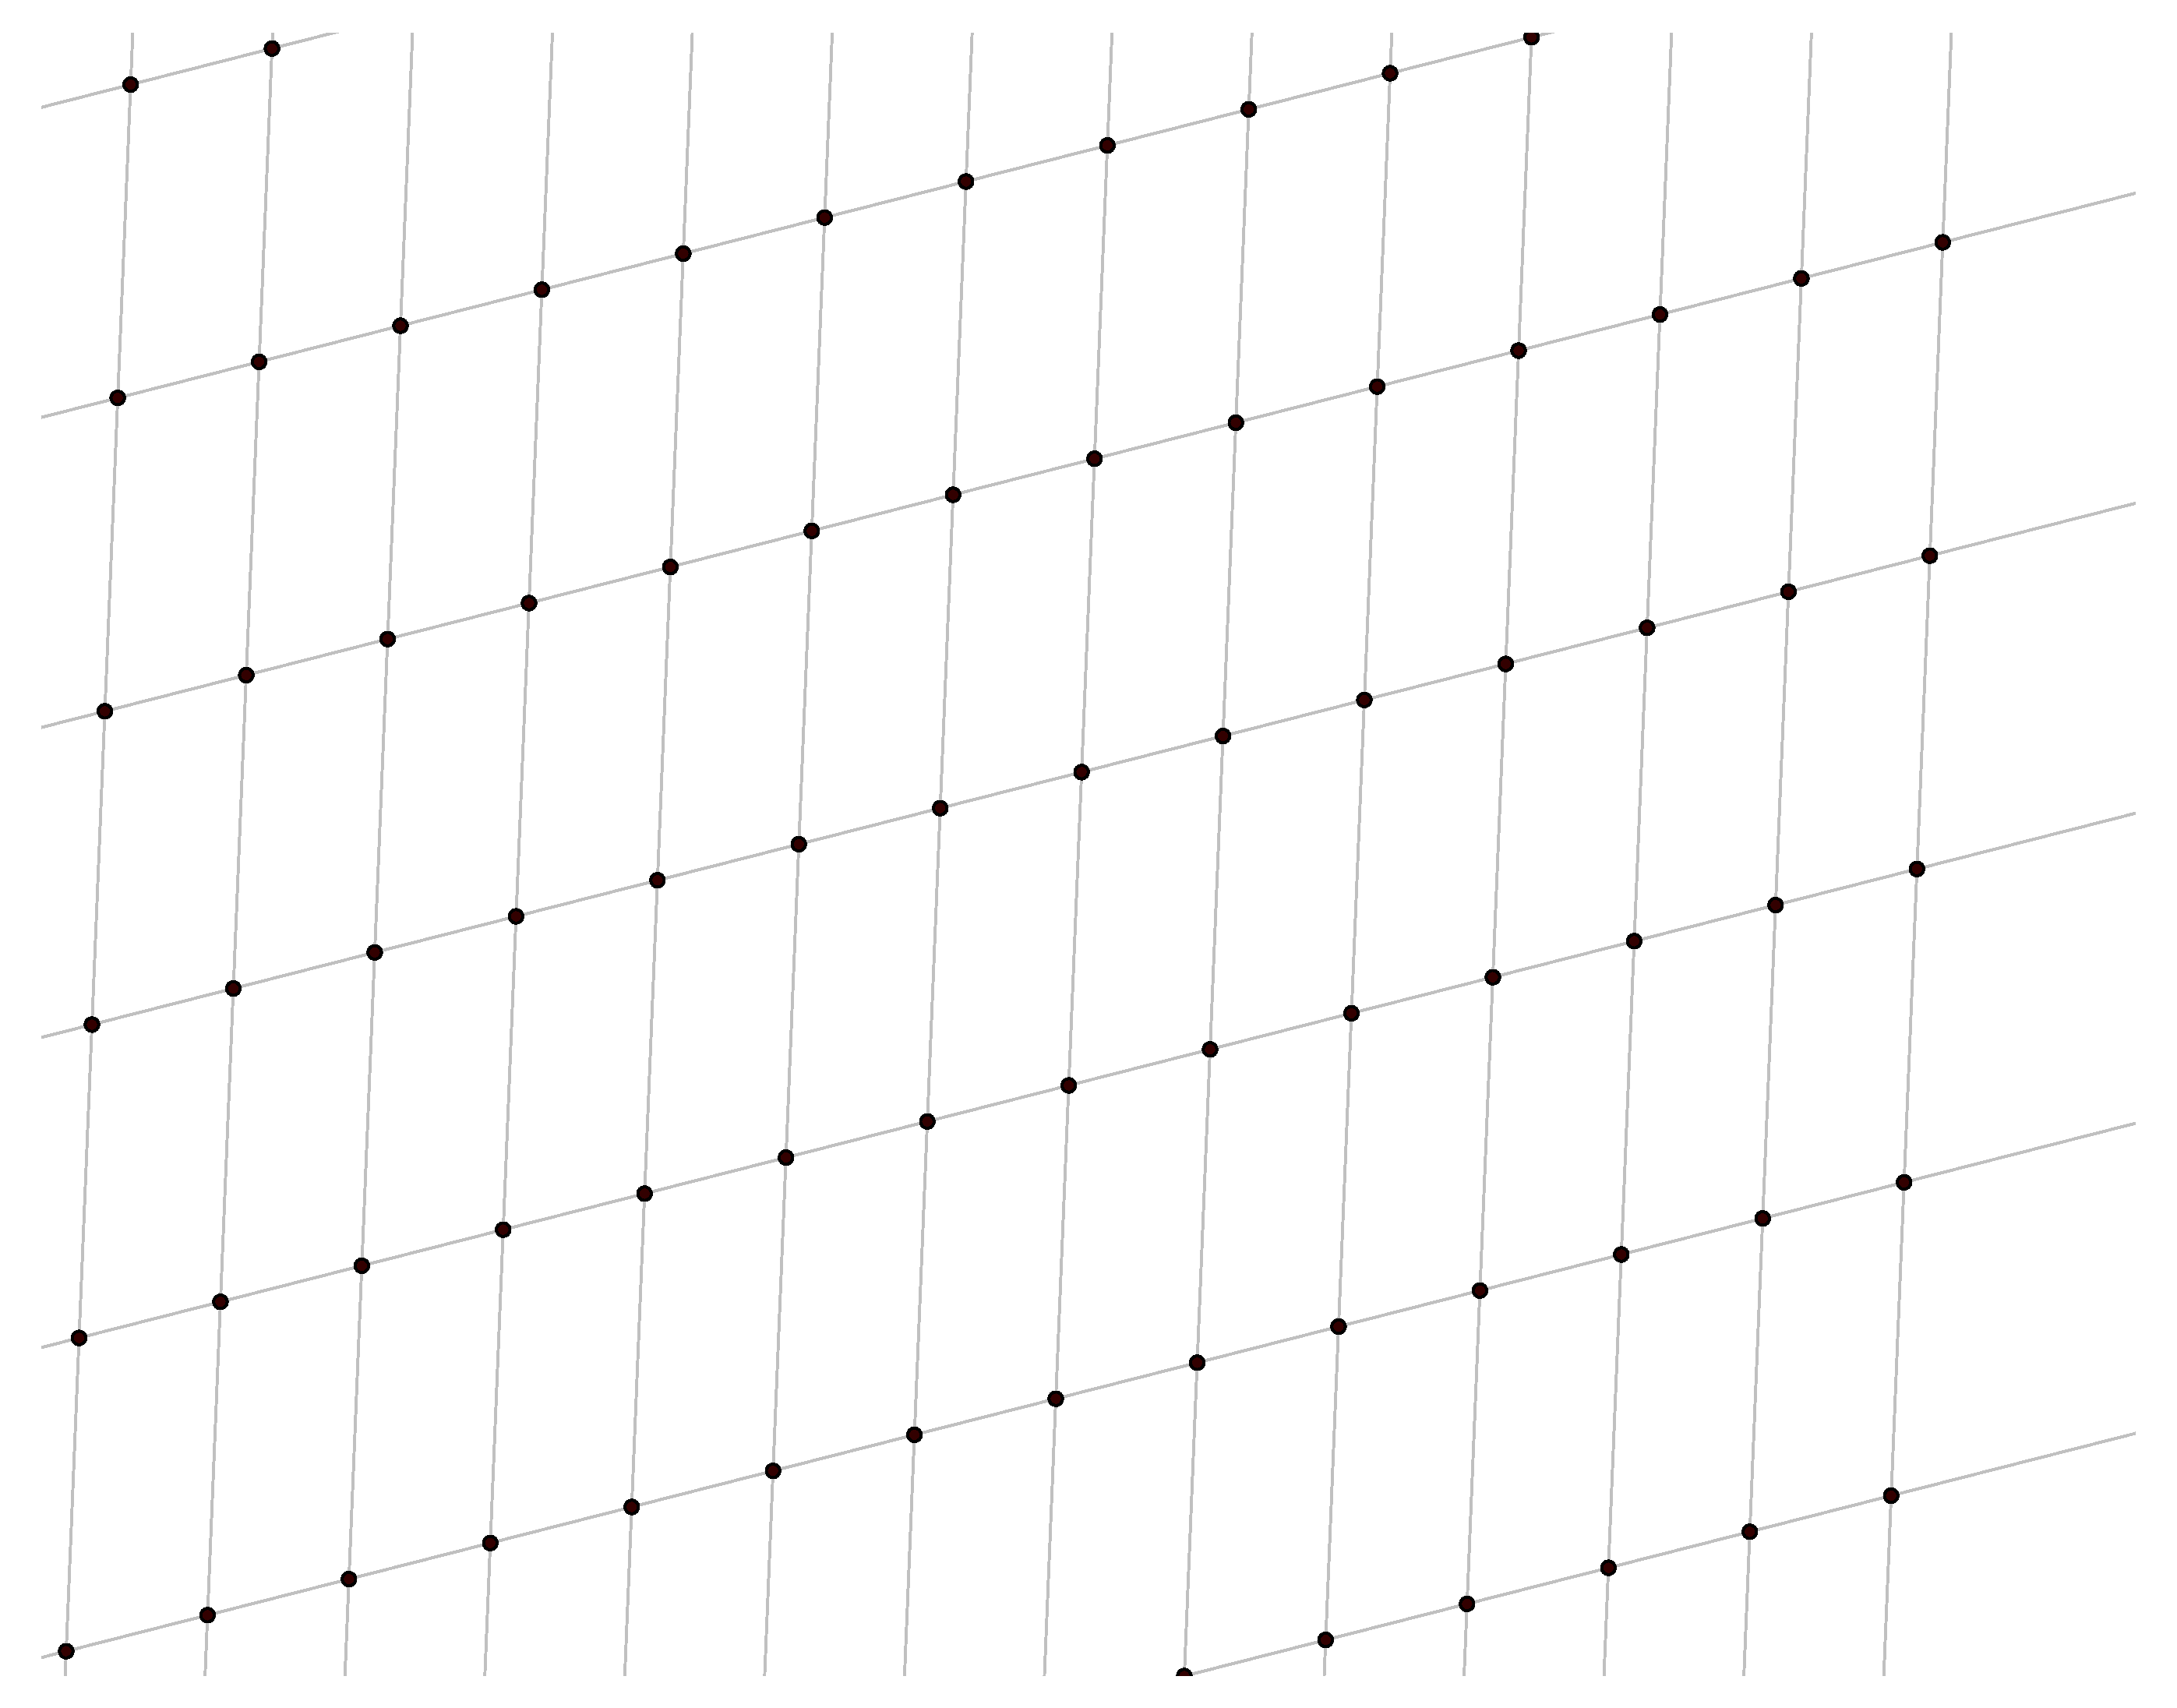
\includegraphics[trim=30 20 180 20, clip, width=\linewidth]{fig/pargrid1.pdf}}
}\end{subfigure}%
\hfill%
\begin{subfigure}{.33\textwidth}
{
	\setlength{\fboxsep}{0pt}%
	\setlength{\fboxrule}{0.5pt}%
	\fbox{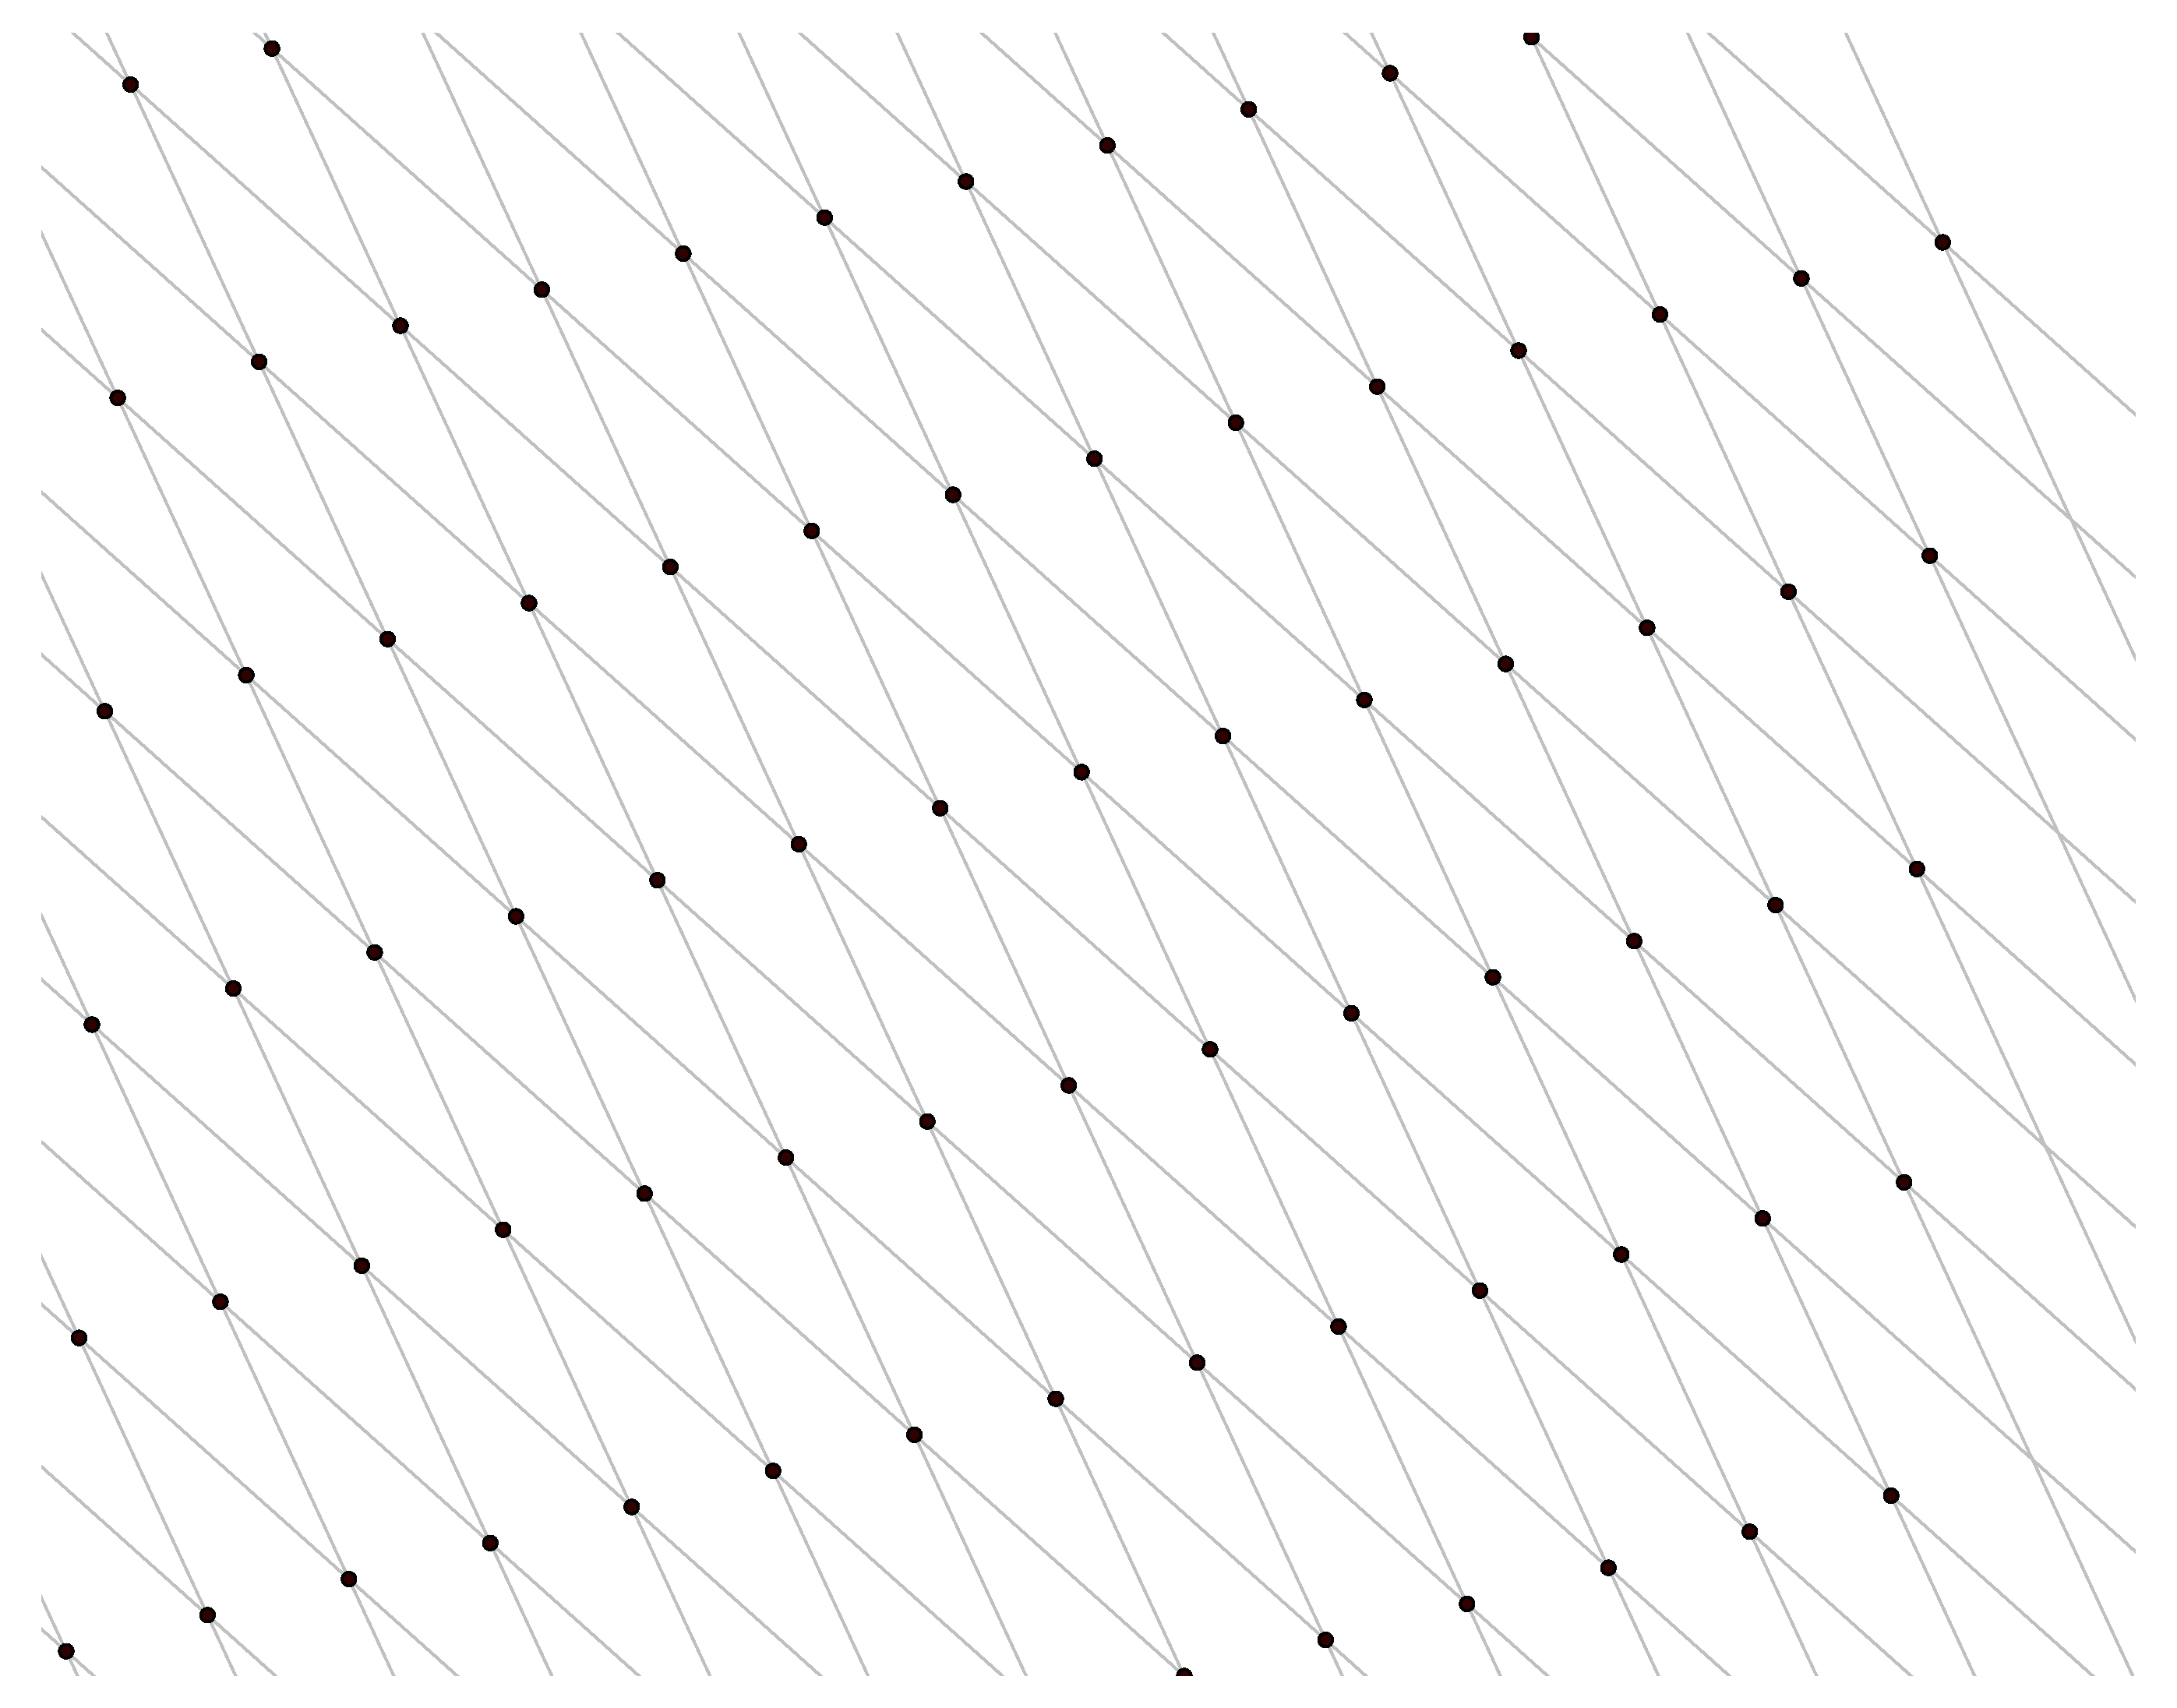
\includegraphics[trim=30 20 180 20, clip, width=\linewidth]{fig/pargrid2.pdf}}
}\end{subfigure}%
\hspace*{\fill}
\caption{Different parallelogram grids for same point dispersion}
\label{fig:par_grid_tilings}
\end{figure}


\subsubsection{Measures}
Three measures on the point dispersion will be used: (1) The point density $\rho$. (2) The shortest possible parallelogram side length $l_{\text{min}}$, for any parallelogram grid put on the points. It corresponds to the distance from any point to its closest neighbor. (3) The maximal distance $d_{\text{max}}$ from any position on the plane to the closest point of the dispersion.

These values can be calculated from the normal vector $\vec{n}$, and the square grid side length on image space $p_l$ as follows. Proofs for these formulea are given in appendix \ref{sec:proof_pargrid_measures}.
\begin{equation}
\rho = \frac{| n_z |}{p^2_l}
\end{equation}
\begin{equation} \label{eq:pargrid_lmin}
l_{\text{min}} = p_l \times \min \left\{
\sqrt{1 + \left( \frac{n_x}{n_z} \right)^2},
\sqrt{1 + \left( \frac{n_y}{n_z} \right)^2},
\sqrt{2 + \left( \frac{n_x + n_y}{n_z} \right)^2},
\sqrt{2 + \left( \frac{n_x - n_y}{n_z} \right)^2}
\right\}
\end{equation} 
\begin{equation}
d_{\text{max}} = p_l \times \min \frac{\sqrt{ (1 \pm 2 \, n_x \, n_y + n^2_z) \, (1 - n^2_y) \, (n^2_y + n^2_z) }}{4 \, n^2_z}
\end{equation} 

\subsubsection{Analysis}
Figure \ref{fig:lmin_plot} shows the value $l_{\text{min}}$, in function of the normal vector $\vec{n}$ of the plane. For the grayscale tones a logarithmic scale is used. Darker tones correspond to lower values. The $x$ and $y$ axis of the plot correspond to $n_x$ and $n_y$, the third component is set to $n_z = \sqrt{1 - n^2_x - n^2_y}$. The plot is symmetric around the X and Y axis. The origin point $(0, 0)$ corresponds to $\vec{n} = \transpose{(0, 0, 1)}$, that is, the plane is perpendicular to the camera ray and has a square grid dispersion. Then $l_{\text{min}} = 1$, the side length of the square. For the points on either axis, the plane is turned on one direction only, resulting in a rectangular grid, where the shortest side remains $l_{\text{min}} = 1$. Around the border of the plot, the plane is nearly parallel to the camera rays. When $n_x \approx n_y$, the parallelograms take on a rhombus shape, similar to the second grid shown on figure \ref{fig:par_grid_tilings}. The shortest edge becomes the projection of the squares' diagonal with length $\sqrt{2}$, whereas the projection of its sides results in longer edges.

\begin{figure}[p]
\centering
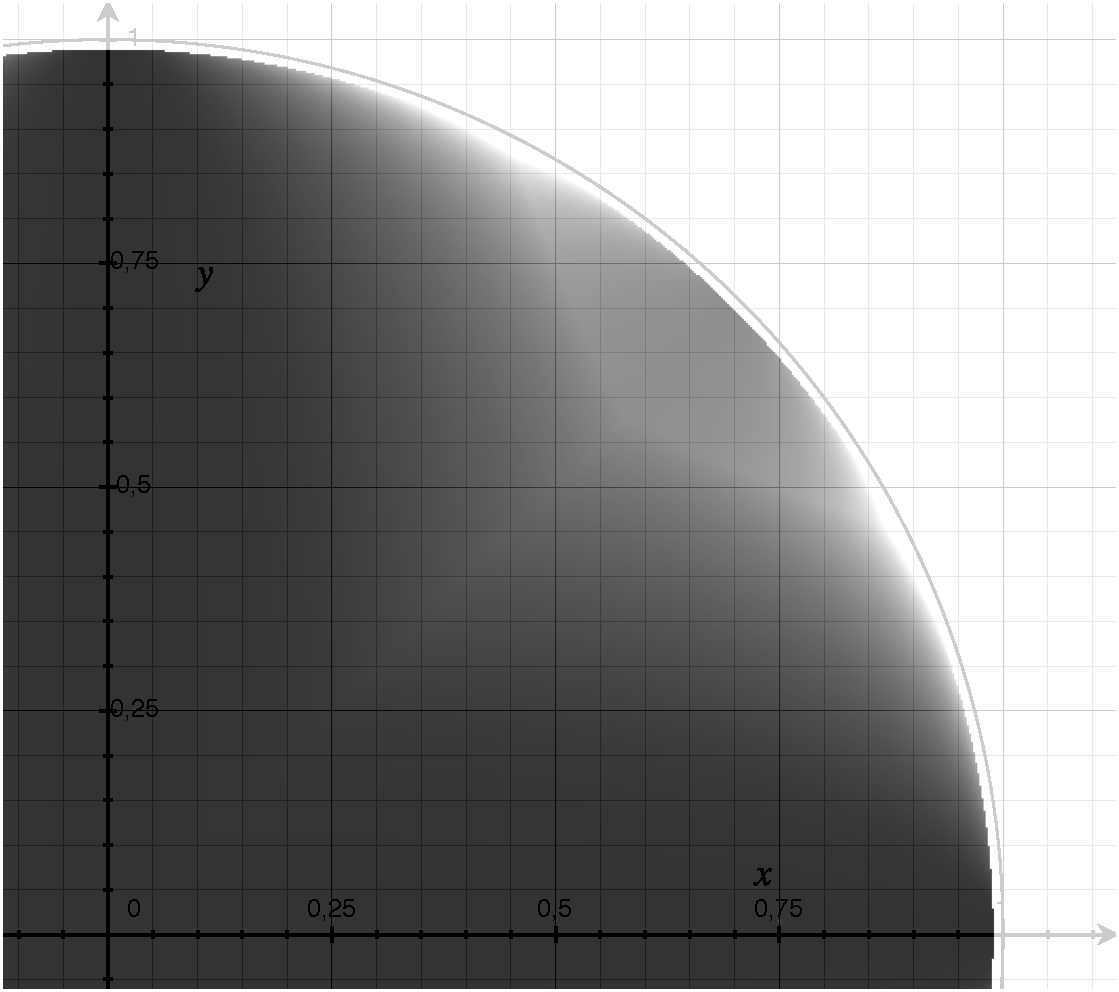
\includegraphics[width=.4\textwidth]{fig/lmin_plot.pdf}
\caption{Plot of $l_{\text{min}}$ for $\vec{n} = \transpose{(x, y, \sqrt{1 - x^2 - y^2})}$ and $p_l = 1$}
\label{fig:lmin_plot}
\end{figure}


\subsubsection{Verification}
The first (left-side) histogram on figure \ref{fig:relief_nn_hist} was generated by recording for each point $p \in P$ on a point cloud, the distance $d$ to its closest neighbor. (That is, the point $p' \in P$ such that $p' \neq p$ and $\| p - p' \|$ is minimal.) The point cloud $P$ used is a ``relief'' model as described before in section \ref{sec:art_relief}, projected without occlusion using a parallel projection camera with $p_l = 0.01$.

Two clusters for around $0.01$ for parts of the surface that are near-parallel to the camera rays, and around $0.0115$, where the surface is more oblique in both directions. Since the surface is not everywhere locally planar the histogram does not form sharp spikes.

For the second histogram the values $l_{\text{min}}$ are instead recorded using the normal vectors of the points $p \in P$, and with fixed $p_l = 0.01$. This histogram is generated solely by evaluating the formula \ref{eq:pargrid_lmin}, without looking at the coordinates of the points, or doing a closest neighbor search in $P$.

\begin{figure}[H]
\centering
\begin{subfigure}{.5\textwidth}
	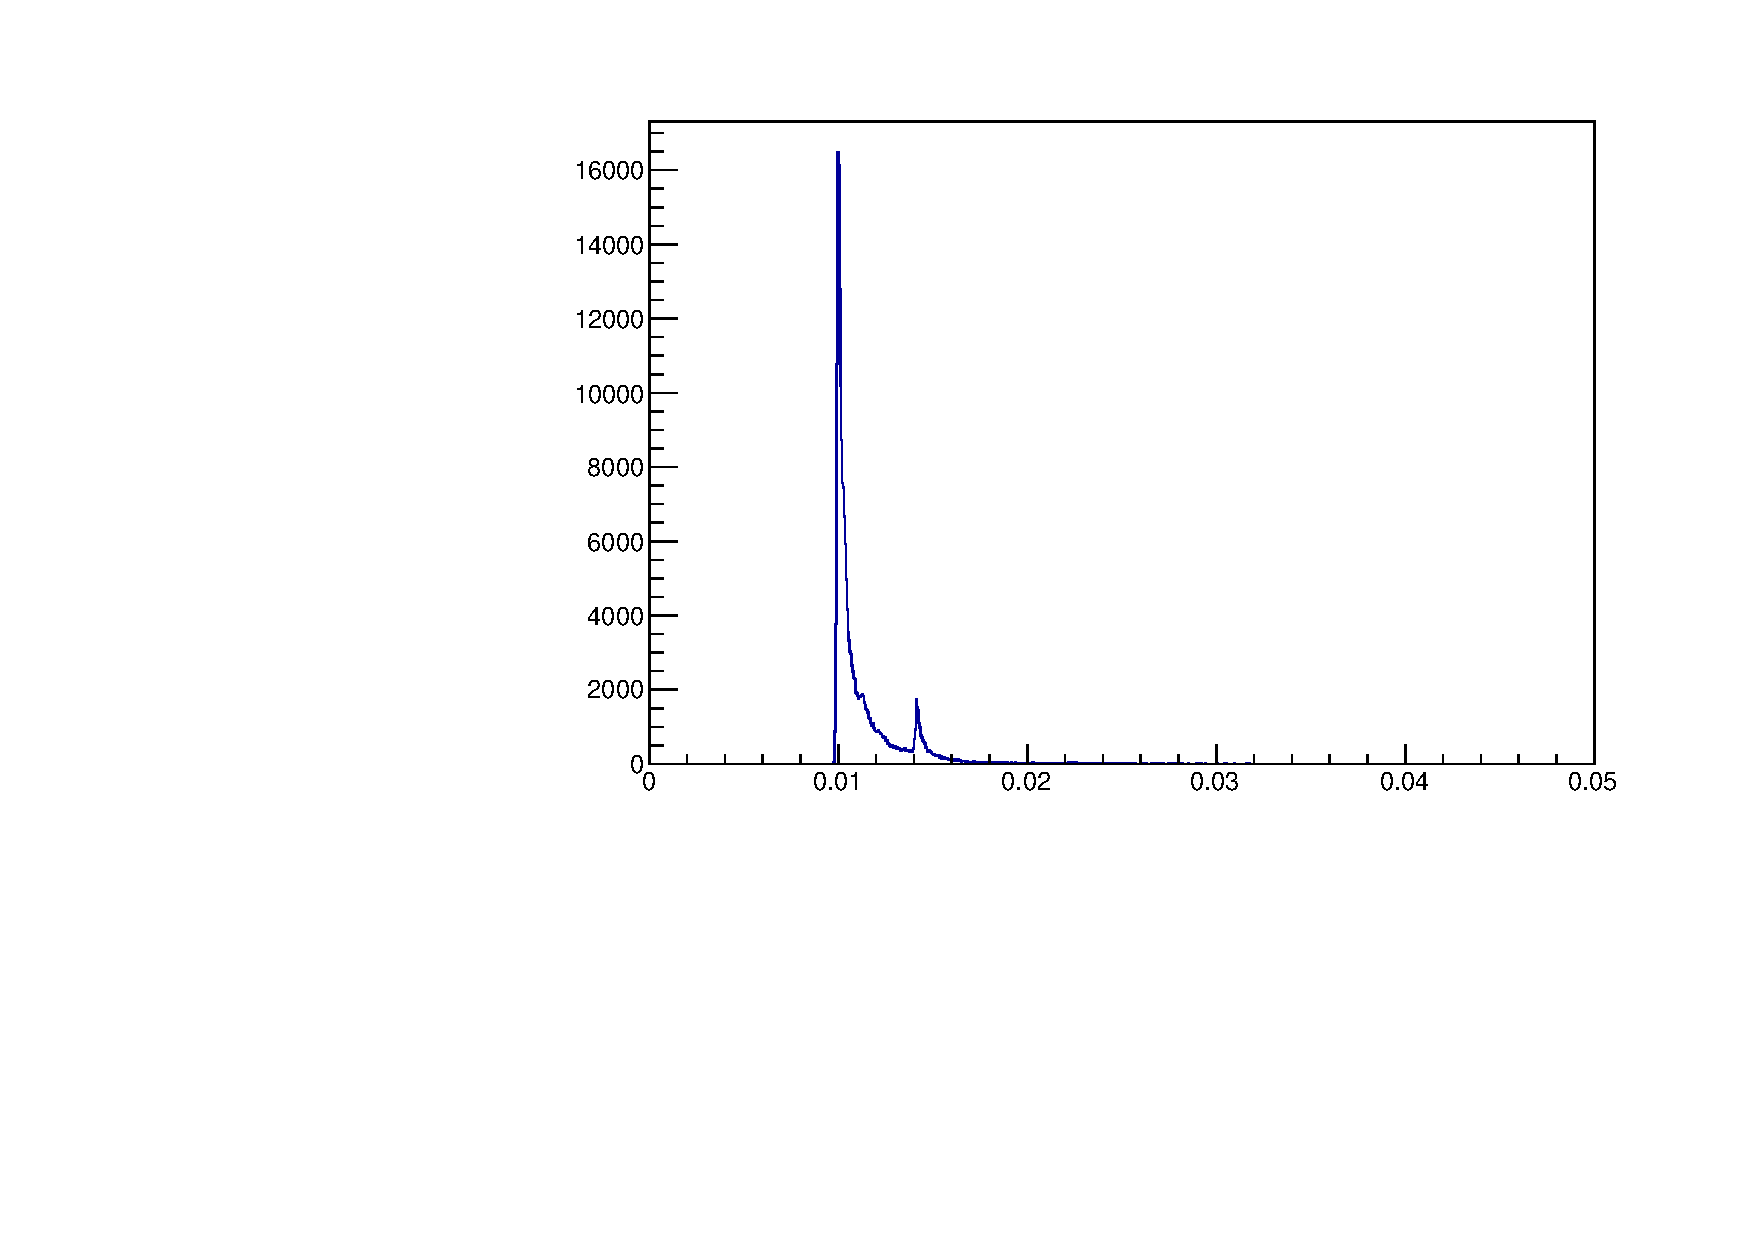
\includegraphics[width=\linewidth]{fig/nn.pdf}
	\caption{Closest neighbor distances on $P$}
\end{subfigure}%
\begin{subfigure}{.5\textwidth}
	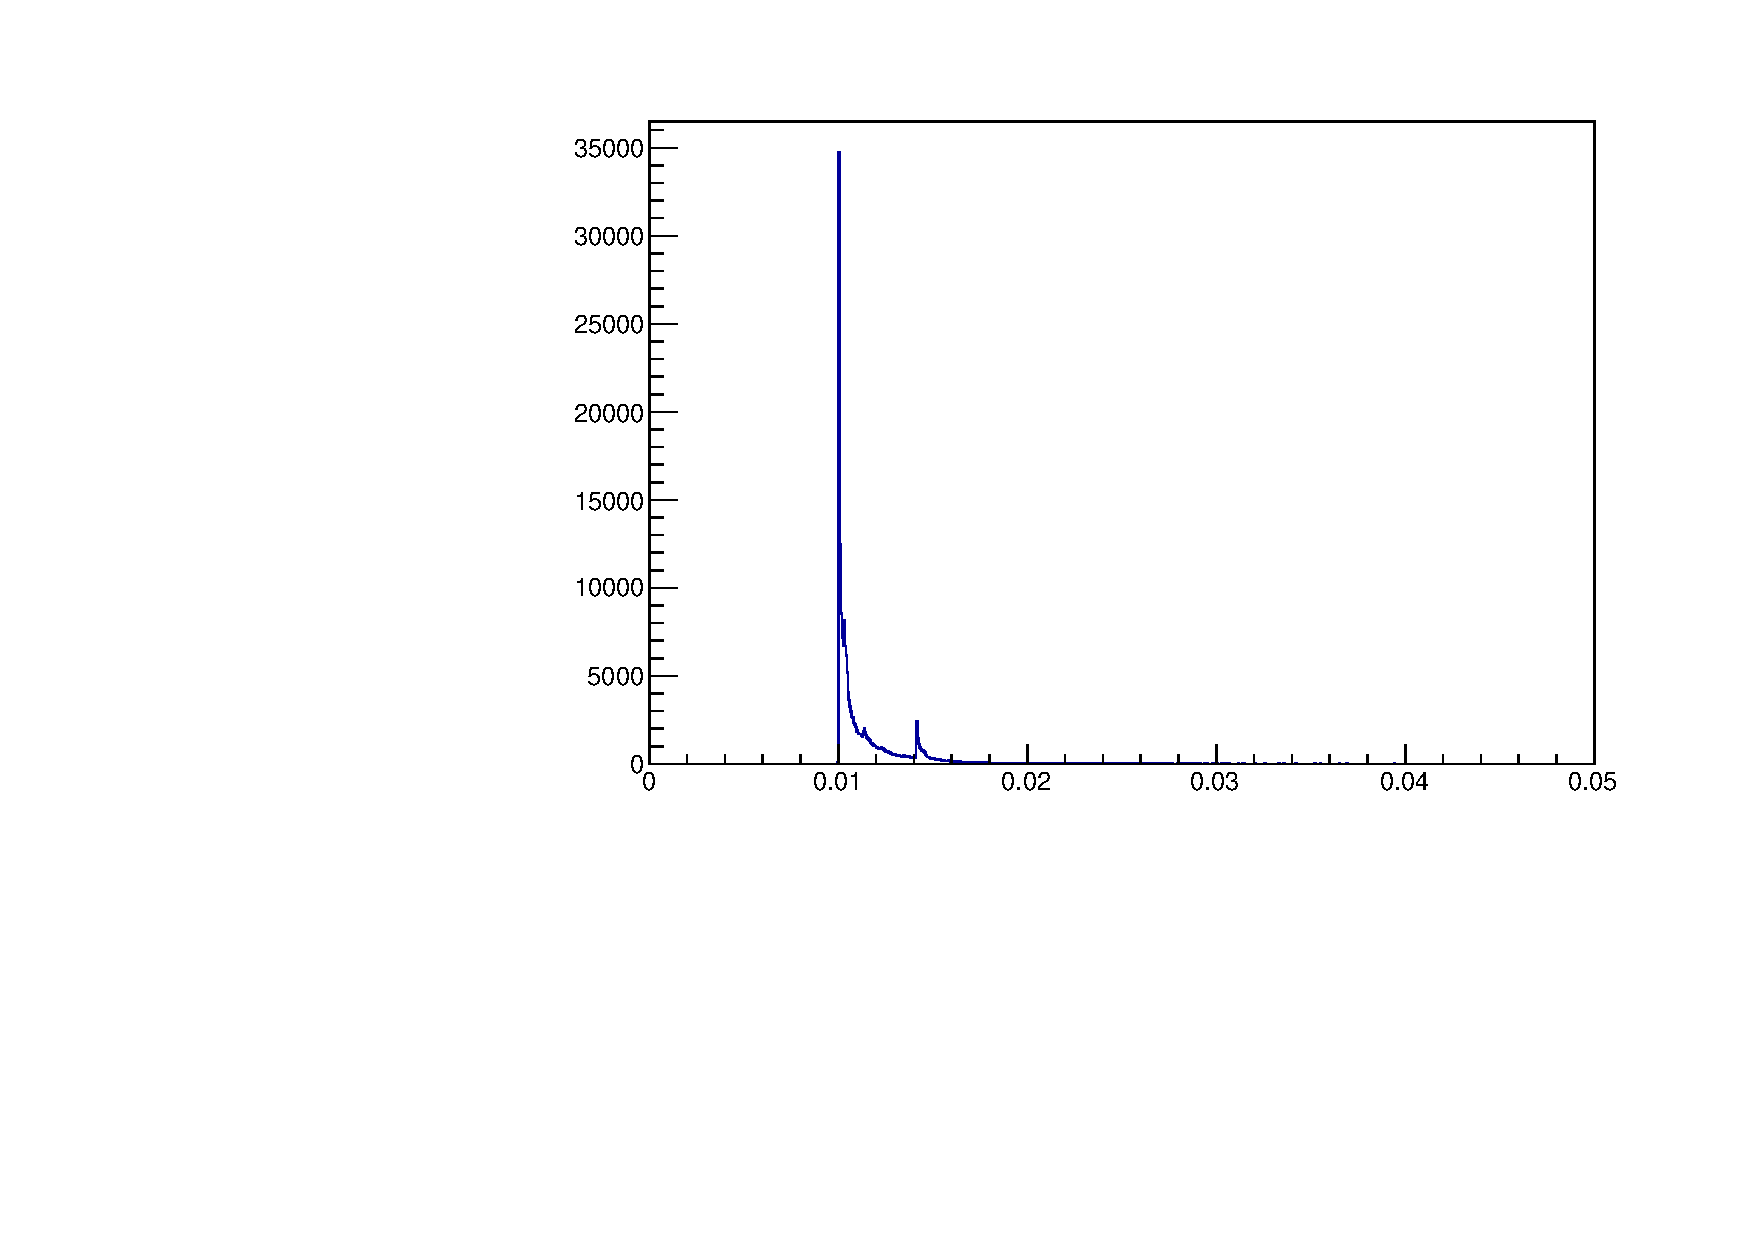
\includegraphics[width=\linewidth]{fig/nn_lmin.pdf}
	\caption{Values $l_{\text{min}}(\vec{n})$ on $P$}
\end{subfigure}	
\caption{Comparison of measured closest neighbor distances and $l_\text{min}$ values.}
\label{fig:relief_nn_hist}
\end{figure}

A similar distribution can be observed on both histograms. The spike at $0.01$ occurs because the camera is placed such that the majority of the surface is approximatively perpendicular to the rays. This confirms the correctness of the formula for $l_{\text{min}}$ for the parallelogram dispersion generated by parallel projection. The similarity of these two histograms also allows for estimation of $p_l$, even when it is not a mode.
 
The correctness of the formula for $d_{\text{max}}$ will be shown in the next section.


\subsection{Projection parameters}
If the point cloud was generated using a parallel projection camera where the graduation in the $x$ and $y$ directions on the image planes is the same, a value $p_l$ exists for the point cloud. This remains true by approximation for small extracts of large 3D scans. In the following the assumption is made that a constant value $p_l$ exists for the entire point cloud.

As shown before, using the properties of the parallelogram grid dispersion and formula \ref{eq:pargrid_lmin}, $p_l$ can be estimated by analyzing the points of the point clouds and their normal vectors. The formula is such that $l_{\text{min}}$ is proportional to $p_l$, and the proportionality constant $m = \min \left\{ \cdots \right\}$ is a function of $\vec{n}$. Assuming that the parallelogram grid covers the entire surface and that the surface is locally planar, $l_{\text{min}}$ can be computed at each point by measuring the distance to the closest neighbor in the point cloud.






\section{Own distance histogram}
Let $P$ and $Q$ be two perfectly aligned point clouds with identical surfaces, but with different point dispersions. They can differ as described in \ref{sec:registration_robostness}. $P$ is called the \emph{model}, and the points $q \in Q$ the \emph{samples}. For each sample $q \in Q$, the closest point $p \in P$ is chosen, and the distance $\|p - q\|$ is recorded. The histogram of these distances will be called the \emph{own distance histogram}. The points $p$ are chosen by the closest point criterion, without additional constraints at first.

In this section the shape of this histogram will be analyzed, and in the next section it will be compared to the \emph{cross distance histogram}, for which $P$ and $Q$ are no longer identical or perfectly aligned.

By replacing the samples $q \in Q$ with a random variable $\textbf{Q}$ with a given probability distribution, the own distance histogram can be idealized into a probability density function of the closest point distance, free of noise resulting from the sparse set of samples.

In the following, $Q$ will be taken to have a much higher point density than $P$. When the number of samples becomes infinite, the histogram converges towards the ideal probability density function. The results will later be applied to devise a method for registering high resolution with low resolution point clouds.

When used on two exact same copies of the same point clouds that are perfectly aligned, all measured distances are $0$, and so the histogram consists only of one spike.

When $P$ is artificial and its surface shape is known, $Q$ is constructed by taking a large number of points on that same surface.

\subsection{Plane with random dispersion}
Figure \ref{fig:plane_rand_d30000} shows an own distance histogram, where $P$ and $Q$ represent a single plane, and the points $p \in P$ are randomly dispersed onto it with an uniform density $\rho(P) = 30000$. For each sample $q$ the distance $d(q, P)$ to the closest point in $P$ is measured. Randomly dispersed means that the $x$ and the $y$ coordinate of each point are chosen randomly and independently, with a uniform distribution in a fixed interval.

Since $P$ and $Q$ are perfectly aligned, in this situation all distances are measured on the two-dimensional plane.

\begin{figure}[H]
\centering
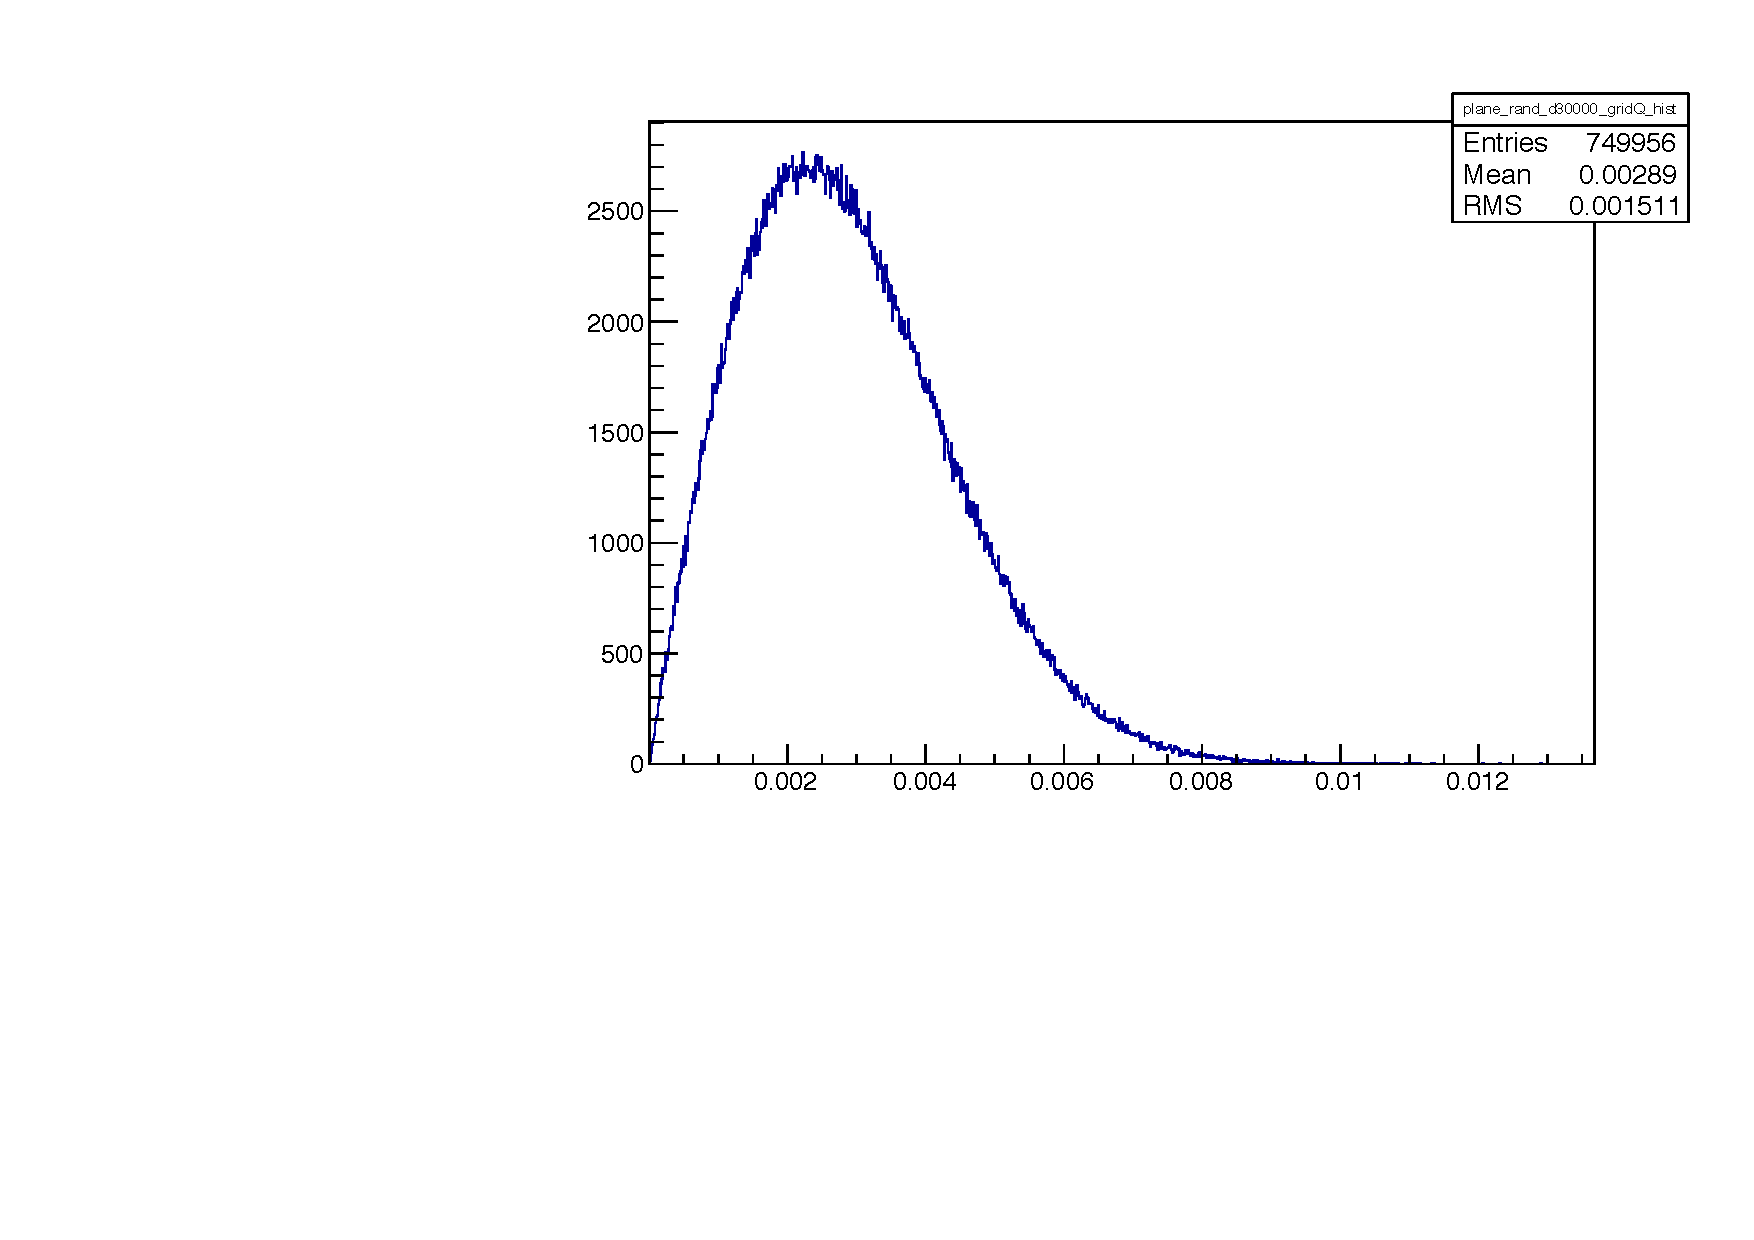
\includegraphics[width=.6\textwidth]{fig/plane_rand_d30000_gridQ.pdf}
\caption{Own distance histogram for plane $P$ with random point distribution}
\label{fig:plane_rand_d30000}
\end{figure}

Unless two points coincide, the probability at $d = 0$ is zero. It then increases, because the probability that a disk with radius $d$ around a sample point $q$ contains at least one $p \in P$ gets larger proportionally to the disk's area. But that disk must increase in radius to contain more than one point, otherwise the closest distance is the distance to the first, closer point inside the disk, and not its radius. This intuitively explains the global shape of the histogram.

The underlying probability density function $f_R$ of the random closest point distance $R$ from any point $q$ is the exponential function
\begin{equation}
f_R(r) = 2 \pi \rho(P) \, r \, e^{-\pi \rho(P) \, r^2}
\end{equation}
This formula is proven in appendix \ref{sec:proof_rand_disp_plane}. A plot is shown in figure \ref{fig:plane_rand_d}, for $\rho(P) = 30000$. It can be seen that the probability density function takes on the same shape as the histogram. By solving $\frac{\diffd}{\diffd r} f_R(r) = 0$, one obtains that the probability density function reaches its maximum at
\begin{equation}
r_{\text{mode}} = \frac{1}{\sqrt{2 \pi} \sqrt{\rho(P)}}
\end{equation}

The mean $\bar{r}$ value for the closest point distance is obtained using the integral
\begin{equation}
\bar{r} = \int_{0}^{\infty} r \, f_R(r) \, \diffd r = \frac{1}{2 \sqrt{\rho(P)}}
\end{equation}

\begin{figure}[p]
\centering
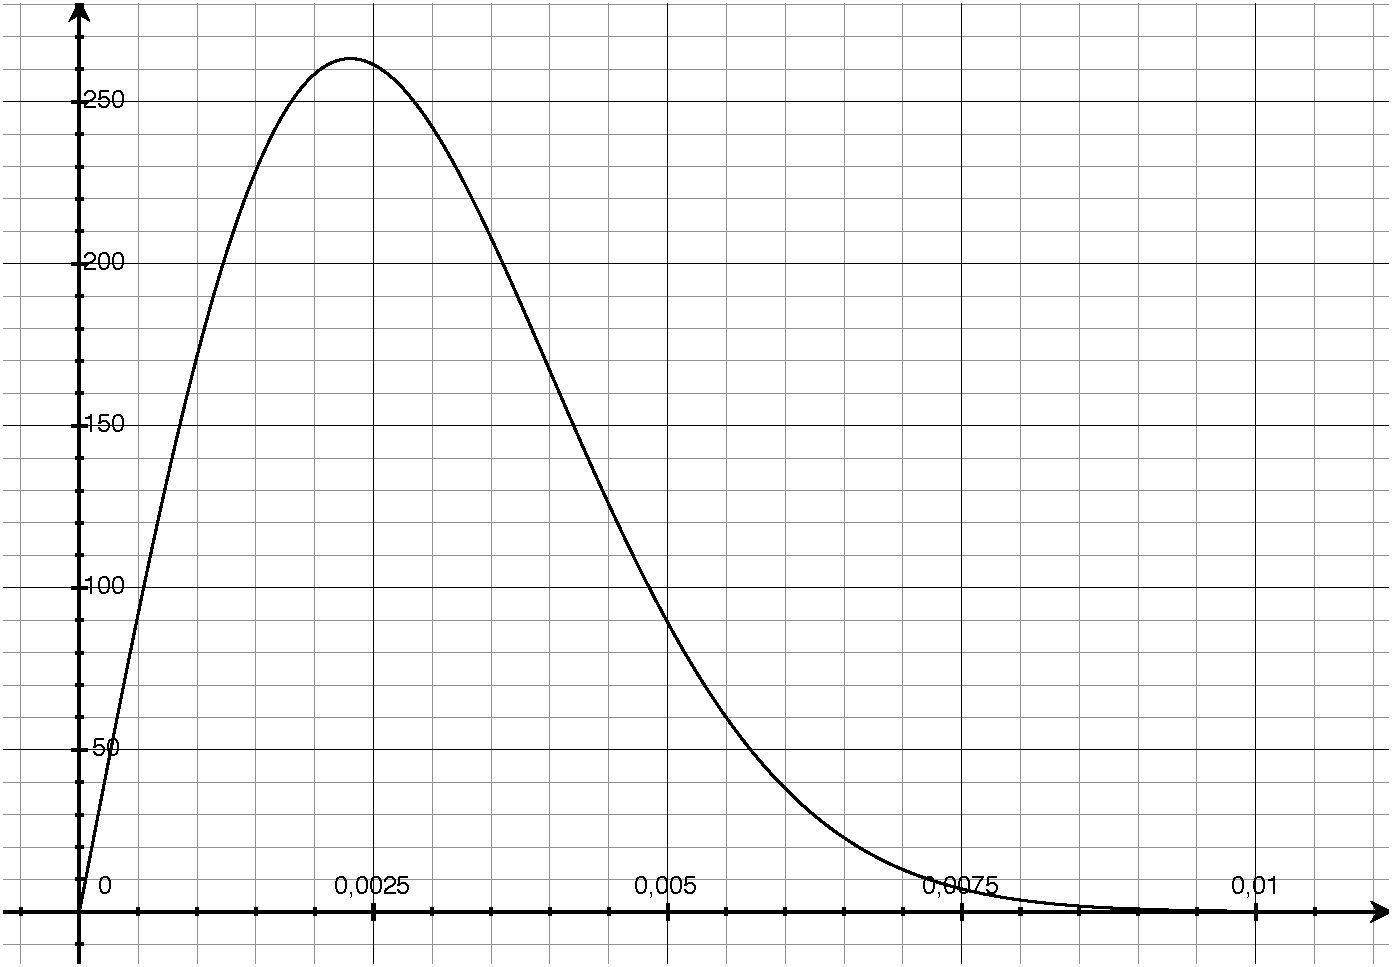
\includegraphics[width=.5\textwidth]{fig/plane_rand_d.pdf}
\caption{Probability density function of closest point distance, for plane $P$ with randomly dispersed points}
\label{fig:plane_rand_d}
\end{figure}

This random points dispersion represents the most general case, where no information about the dispersion of sample points on the surfaces is known. 



\subsection{Dispersion of sample points}
In order to obtain a histogram that closely resembles the theoretical probability density function, the dispersion of the sample points $q \in Q$ should be such that its density is much higher than that of the model points, and has a low variance. If the density is not high enough, the range of possible placements of sample points relative to surrounding model points is sampled too sparsely, leading to a low resolution histogram. If the variance is too high, some placements will be oversampled in comparison to others, and the histogram will contain more noise.

Figure \ref{fig:plane_rand_d30000_randQ} shows the same histogram, but with the sample points $q_i \in Q$ also being randomly dispersed on the plane (and a different number of samples). It is shown in appendix \ref{sec:proof_var_rand_pt_disp} that the local density is not constant.

This effect is greatly reduced when the sample points on $Q$ are instead dispersed on a regular square grid. The deviation of $N(A)$ from $\bar{N}(A)$ then occurs only due to aliasing near the border of the region $A$, so the variance is near-zero. It gets lower with a higher density of the samples $q \in Q$ and consequently lower side length of the square grid. This was used to obtain the histogram \ref{fig:plane_rand_d}.

\begin{figure}[p]
\centering
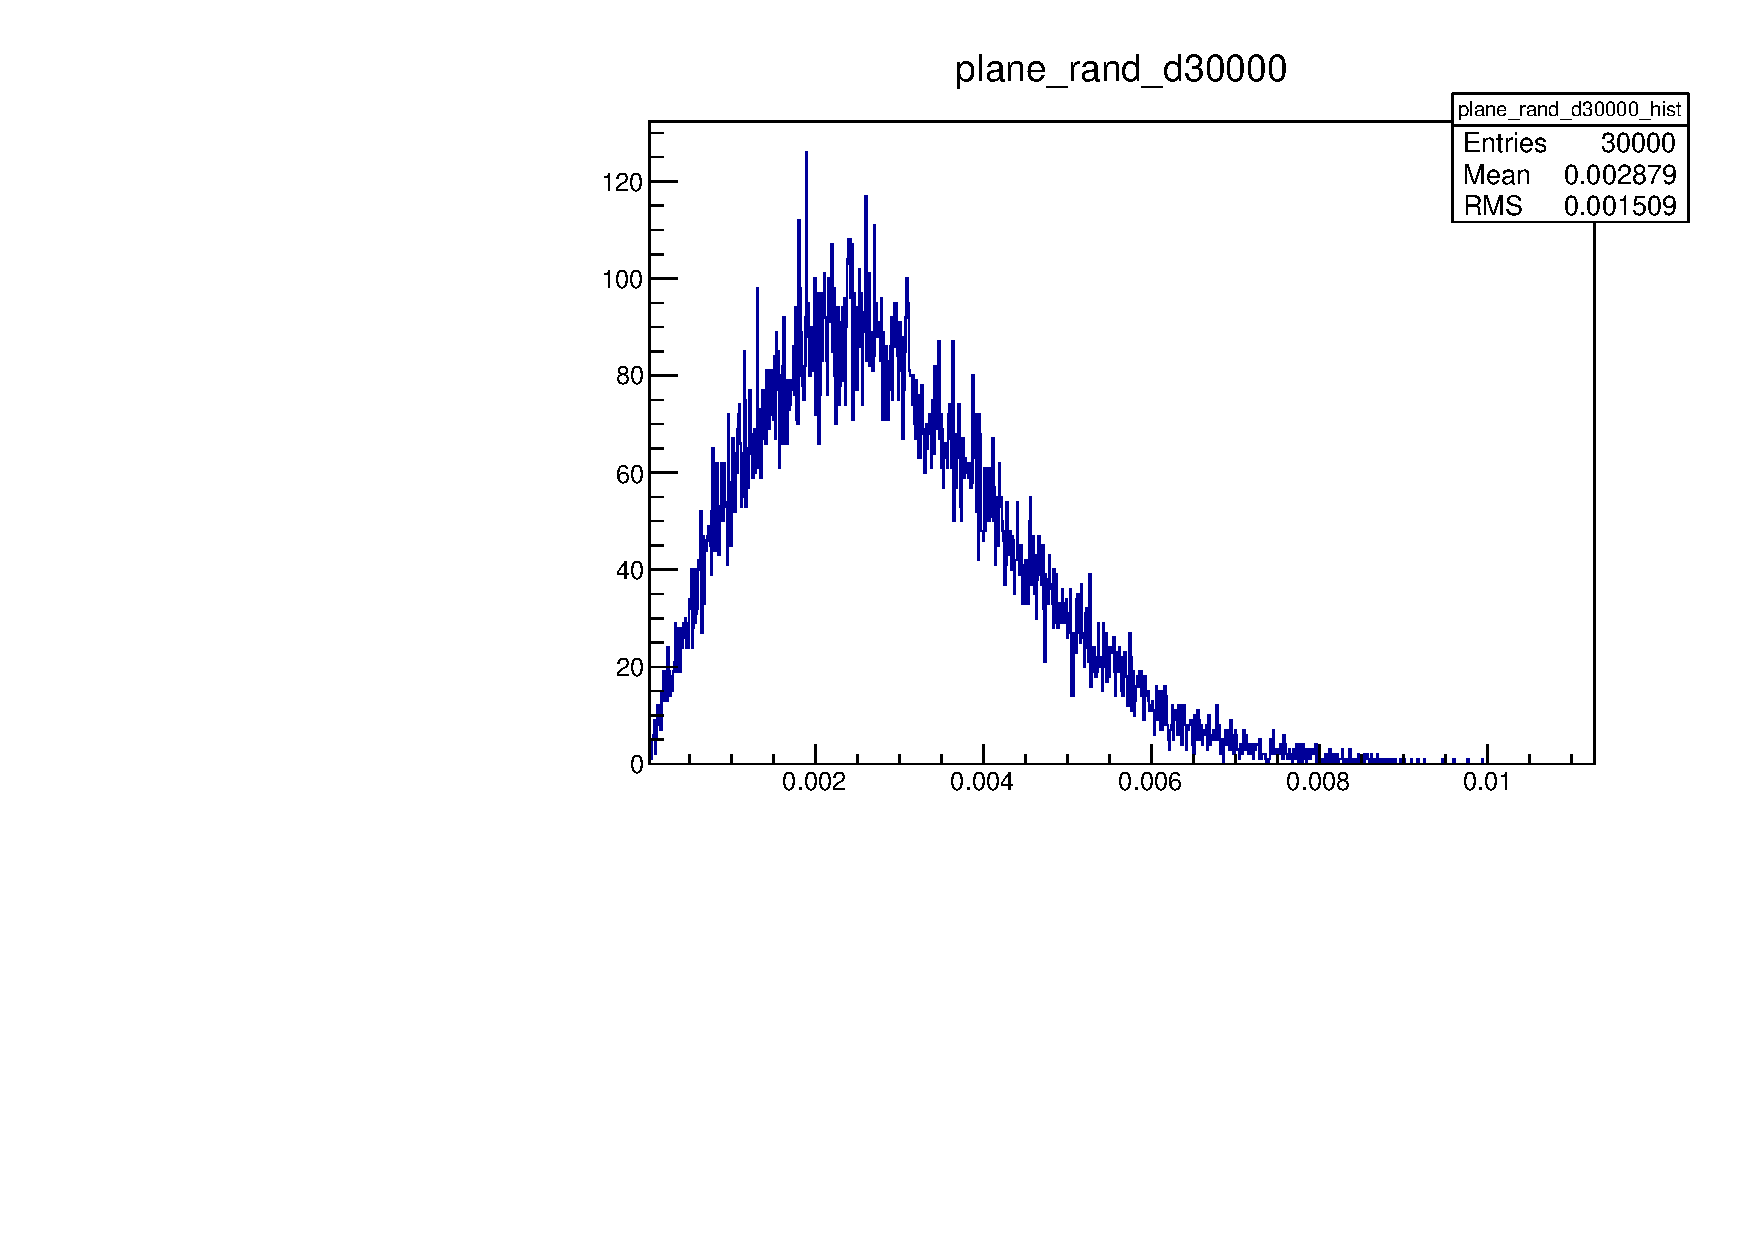
\includegraphics[width=.6\textwidth]{fig/plane_rand_d30000.pdf}
\caption{Same as figure \ref{fig:plane_rand_d30000} but with randomly dispersed samples $q \in Q$}
\label{fig:plane_rand_d30000_randQ}
\end{figure}


When working with artificially generated, perfectly aligned point clouds with a square grid point dispersion, the side lengths $l_P$ and $l_Q$ for the model and the sample point clouds must be chosen such that $\frac{l_P}{l_Q} \notin \mathbb{Q}$, otherwise same placements of sample points relative to model points will repeat, and a larger number of sample points doesn't increase histogram quality. For example if $l_P = 0.1$ and $l_Q = 0.02$, each square of the model will have $25$ sample points placed within it at the same relative positions. Taking into account that floating point numbers with limited precision are used, it means that when considering $l_P$ and $l_Q$ to be rational numbers, they should be chosen such that their least common multiple should is as high as possible.


\subsection{Plane with square grid dispersion}
Figure \ref{fig:plane_cphist} shows the distance histogram of two perfectly aligned planar surfaces $P$ and $Q$, where the points on $P$ are dispersed on a square grid. $\rho(P) = 20000$ and $30000$, respectively. The number of samples is $N(Q) = 300000$.

\begin{figure}[H]
\centering
\begin{subfigure}{.5\textwidth}
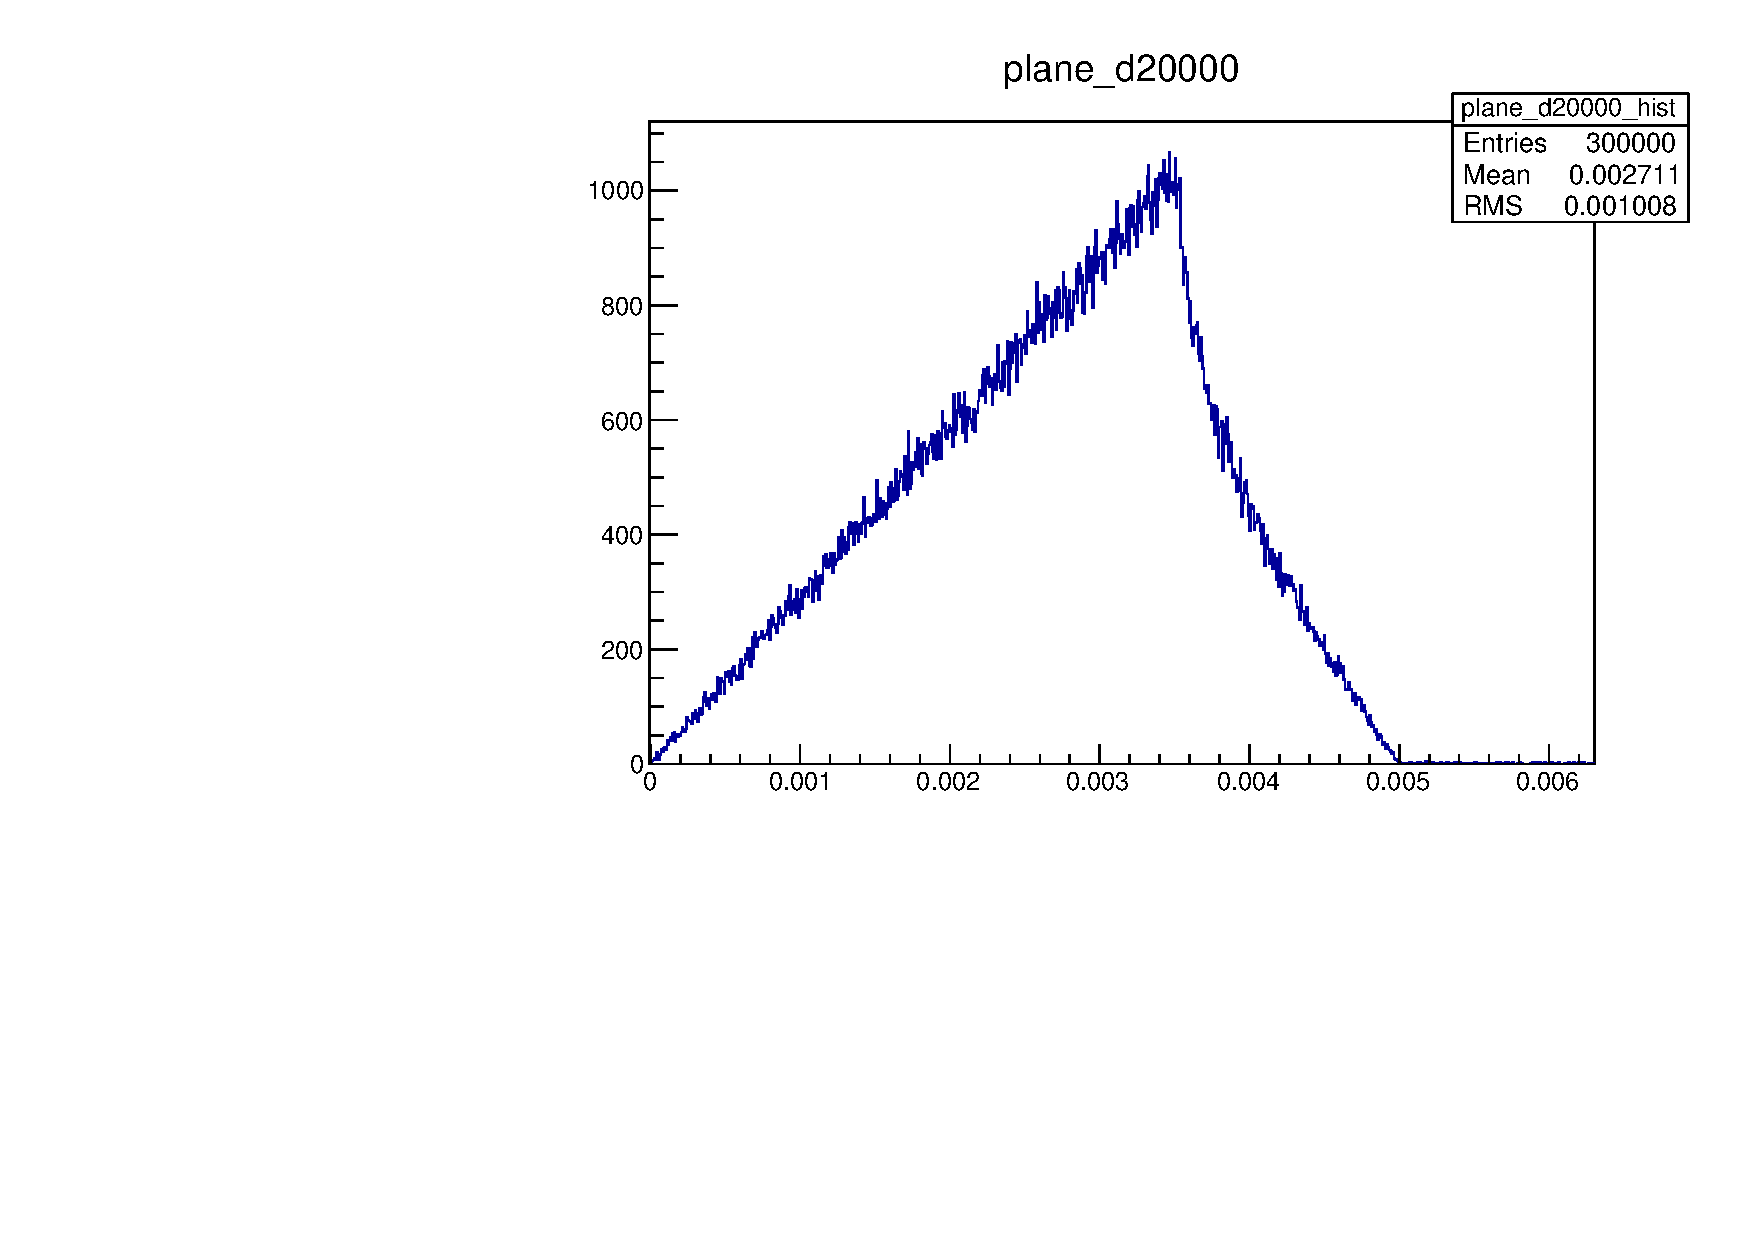
\includegraphics[width=\linewidth]{fig/plane_d20000.pdf}
\end{subfigure}%
\begin{subfigure}{.5\textwidth}
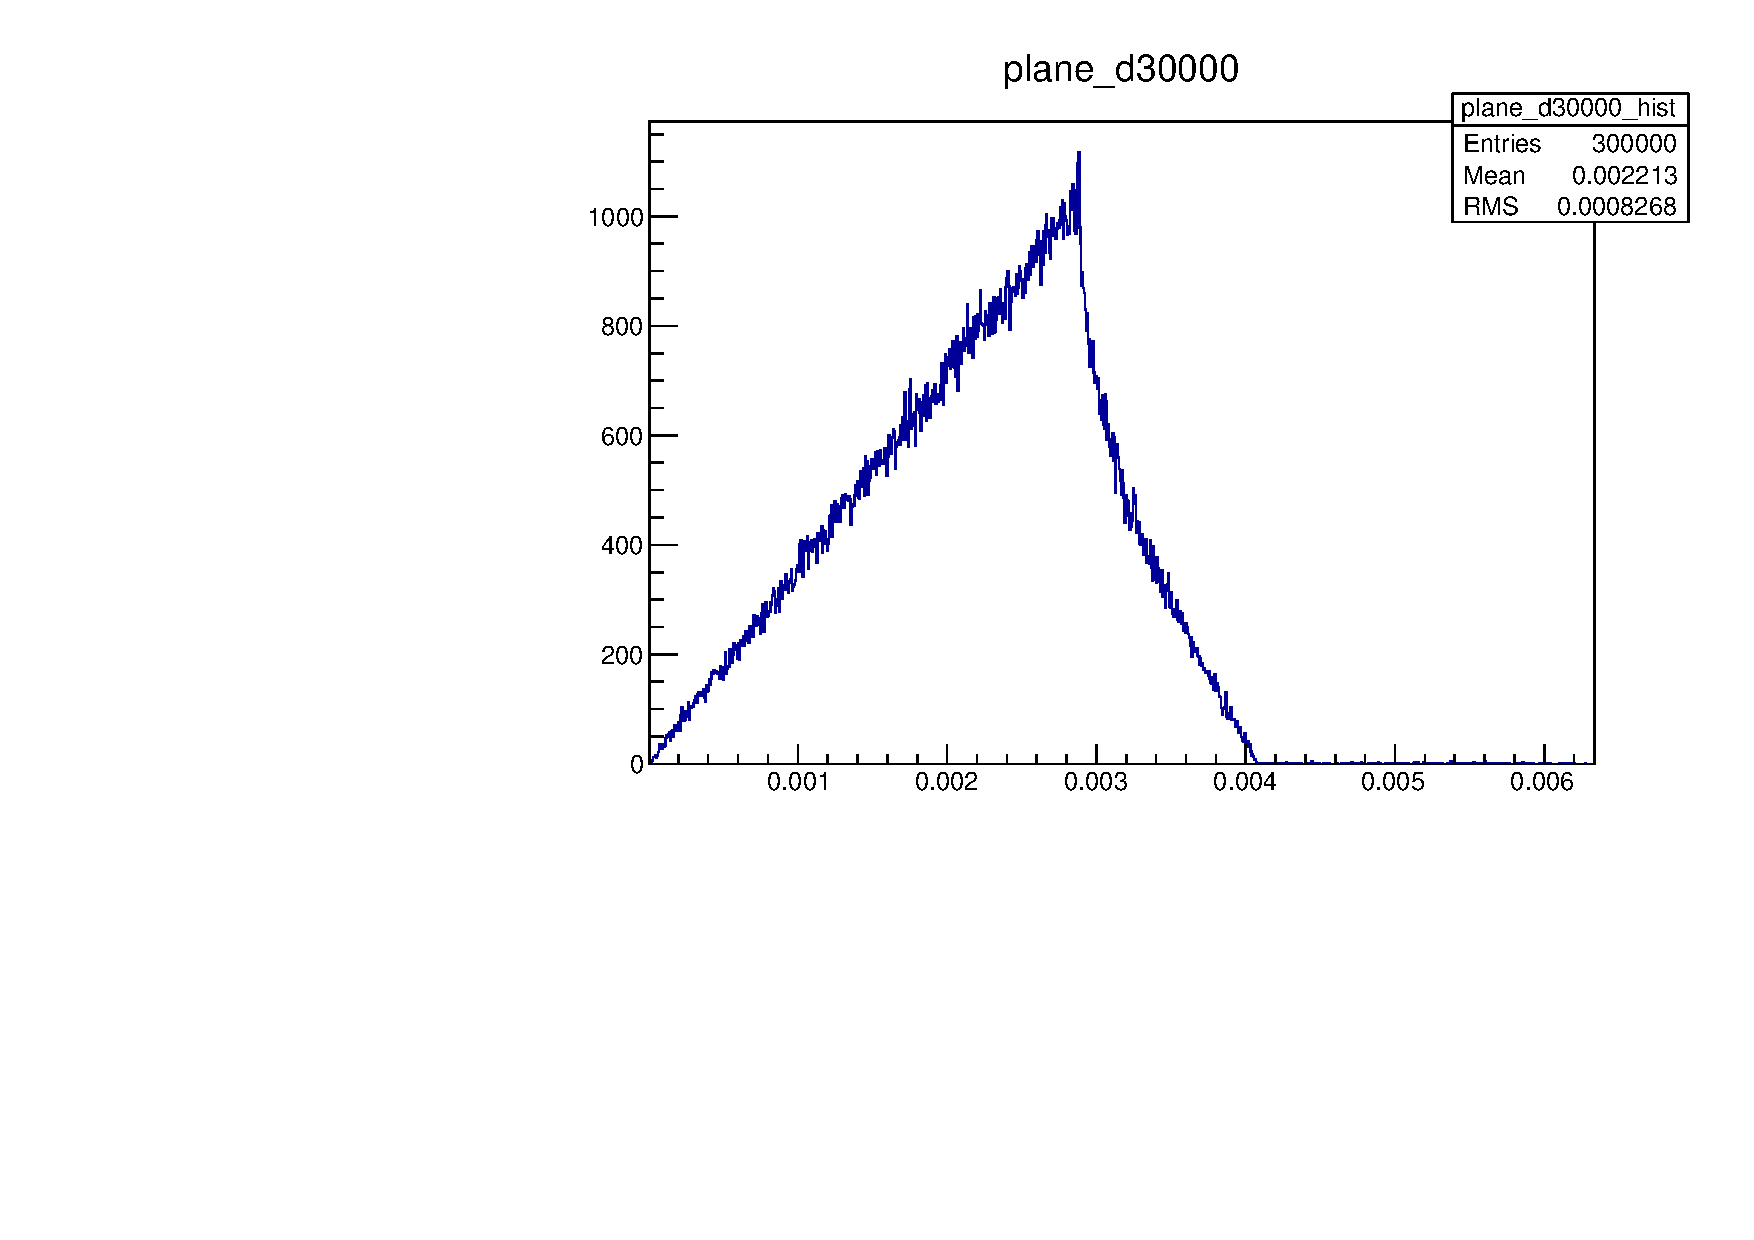
\includegraphics[width=\linewidth]{fig/plane_d30000.pdf}
\end{subfigure}
\caption{Own distance histogram for plane $P$ with square grid point dispersion}
\label{fig:plane_cphist}
\end{figure}

The probability density function $f_R$ is
\begin{equation}
f_R(r) = \frac{r}{2 l} \times \begin{cases}
	\frac{\pi}{4} & 0 \leq r \leq \frac{l}{2} \\
	\frac{\pi}{4} - \arctan{\sqrt{\left( \frac{2r}{l} \right)^2 - 1}} & \frac{l}{2} < r < \frac{l}{2} \sqrt{2}
\end{cases}
\end{equation}
with $l = \frac{1}{\sqrt{\rho(P)}}$. This is proven in appendix \ref{sec:proof_sqgrid_disp_plane}. The plot is shown in figure \ref{fig:sq_grid_d} for $l = 2$.

The probability rises linearily from $O$ to to its mode at $r = \frac{l}{2}$. Within that range, the sample point falls within the non-overlapping disks of radius $\frac{l}{2}$ around the model points. A similar characteristic linear increase exists for parallelogram grid dispersion, and for non-planar surfaces, when $P$ and $Q$ are aligned. This will be used to define a registration accuracy measure.

\begin{figure}[p]
\centering
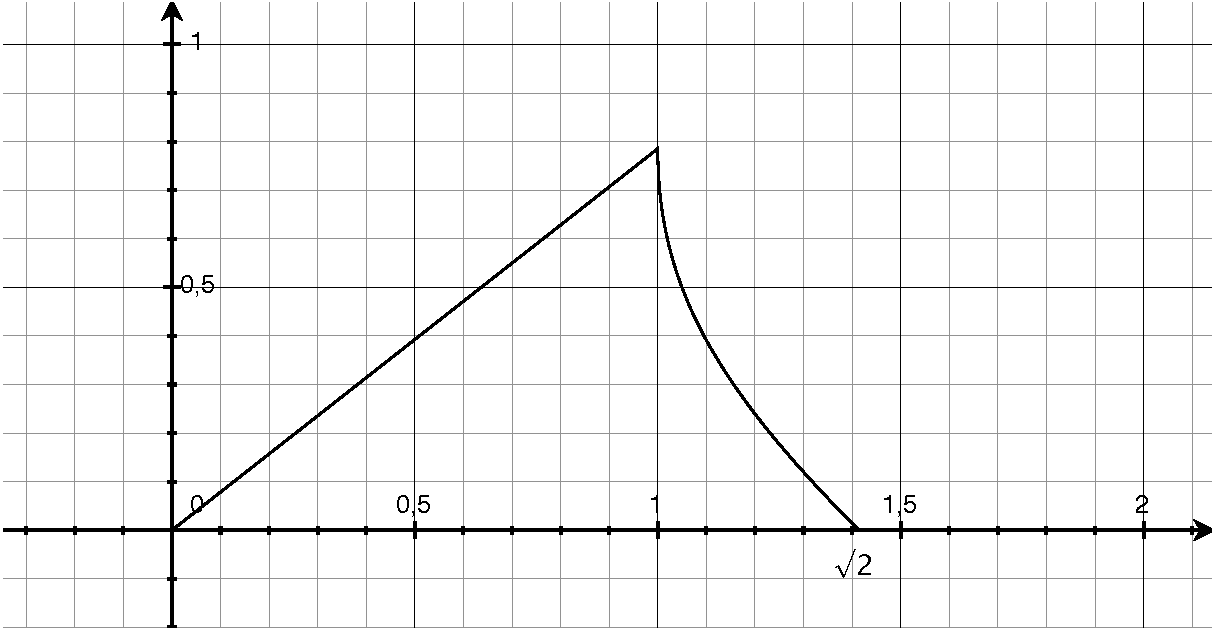
\includegraphics[width=.5\textwidth]{fig/sq_grid_d.pdf}
\caption{Probability density function of closest point distance, for plane $P$ with square grid point arrangement}
\label{fig:sq_grid_d}
\end{figure}


\subsection{Plane with parallelogram grid dispersion}
The square grid dispersion in a special case of the parallelogram grid dispersion. Figure \ref{fig:plane_par_cphist} shows an example of an own closest point histogram obtained when the model point cloud has a parallelogram grid point dispersion. As seen on figure \ref{fig:pargrid_proj}, it is the result of a parallel projection of a square grid on the camera image frame onto a plane in space with a normal vector $\vec{n}$, relative to the camera's coordinate system. For this example, $\vec{n} \approx \transpose{(-0.253023, 0.787174, -0.562438)}$, and the square grid on the image plane has a side length of $p_l = 0.067$.
s
Figure \ref{fig:par_grid} is a close-up view of the plane, showing the parallelogram grid of $P$, and the higher density square grid sample point cloud $Q$ in blue.


\begin{figure}[H]
\centering
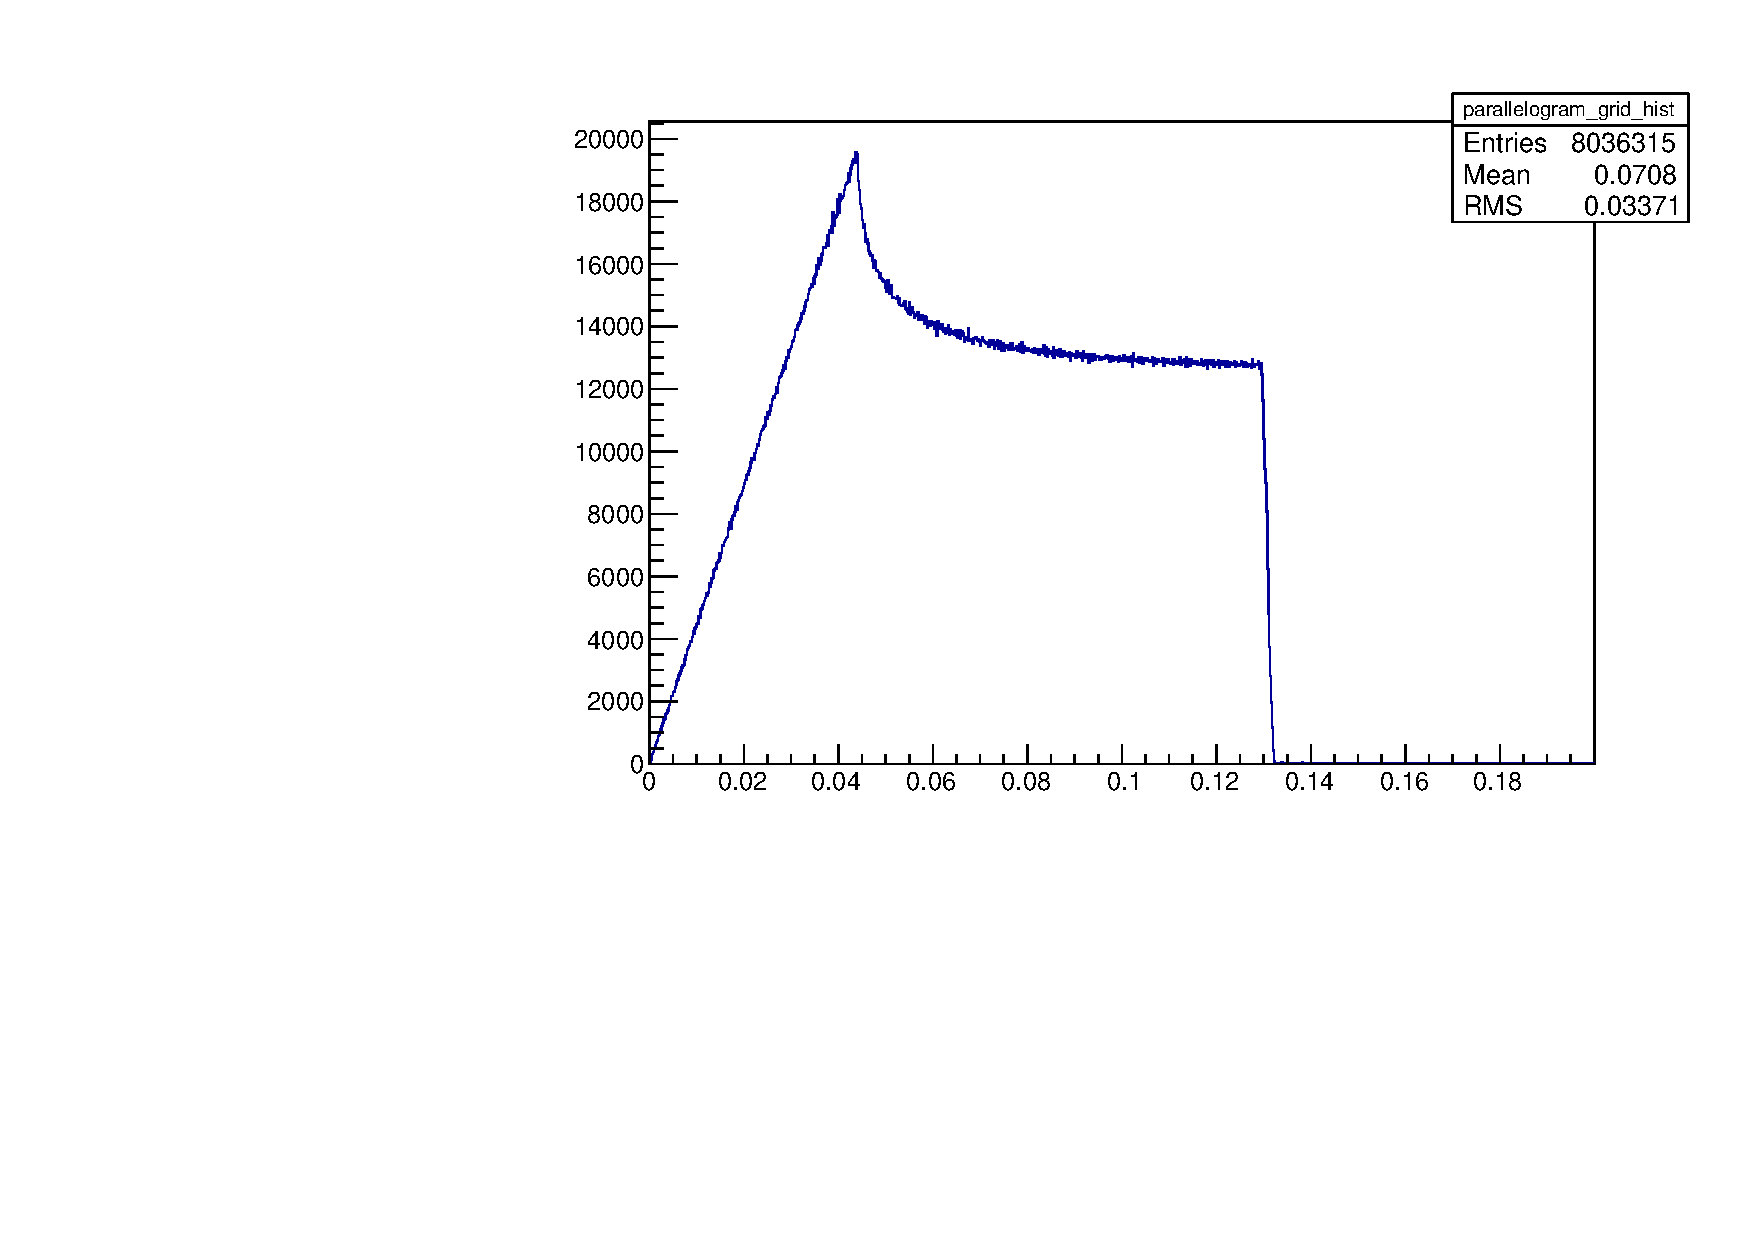
\includegraphics[width=.5\textwidth]{fig/parallelogram_grid.pdf}
\caption{Own distance histogram for plane $P$ with parallelogram grid point dispersion}
\label{fig:plane_par_cphist}
\end{figure}

It can be seen that the histogram's underlying probability density function is again a piecewise function, and that its first segment is still a linear increase from the zero point to the mode of the histogram.

Using a similar argument as for the square grid dispersion, one can show that the linear increase happens from $0$ to $\frac{1}{2} l_\text{min}$. Applying the formula \ref{eq:pargrid_lmin} developed in the previous section, a value of approximatively $0.0441$ is found for this example. It corresponds to the mode seen on the histogram.

\begin{figure}[p]
\centering
{
	\setlength{\fboxsep}{0pt}%
	\setlength{\fboxrule}{0.5pt}%
	\fbox{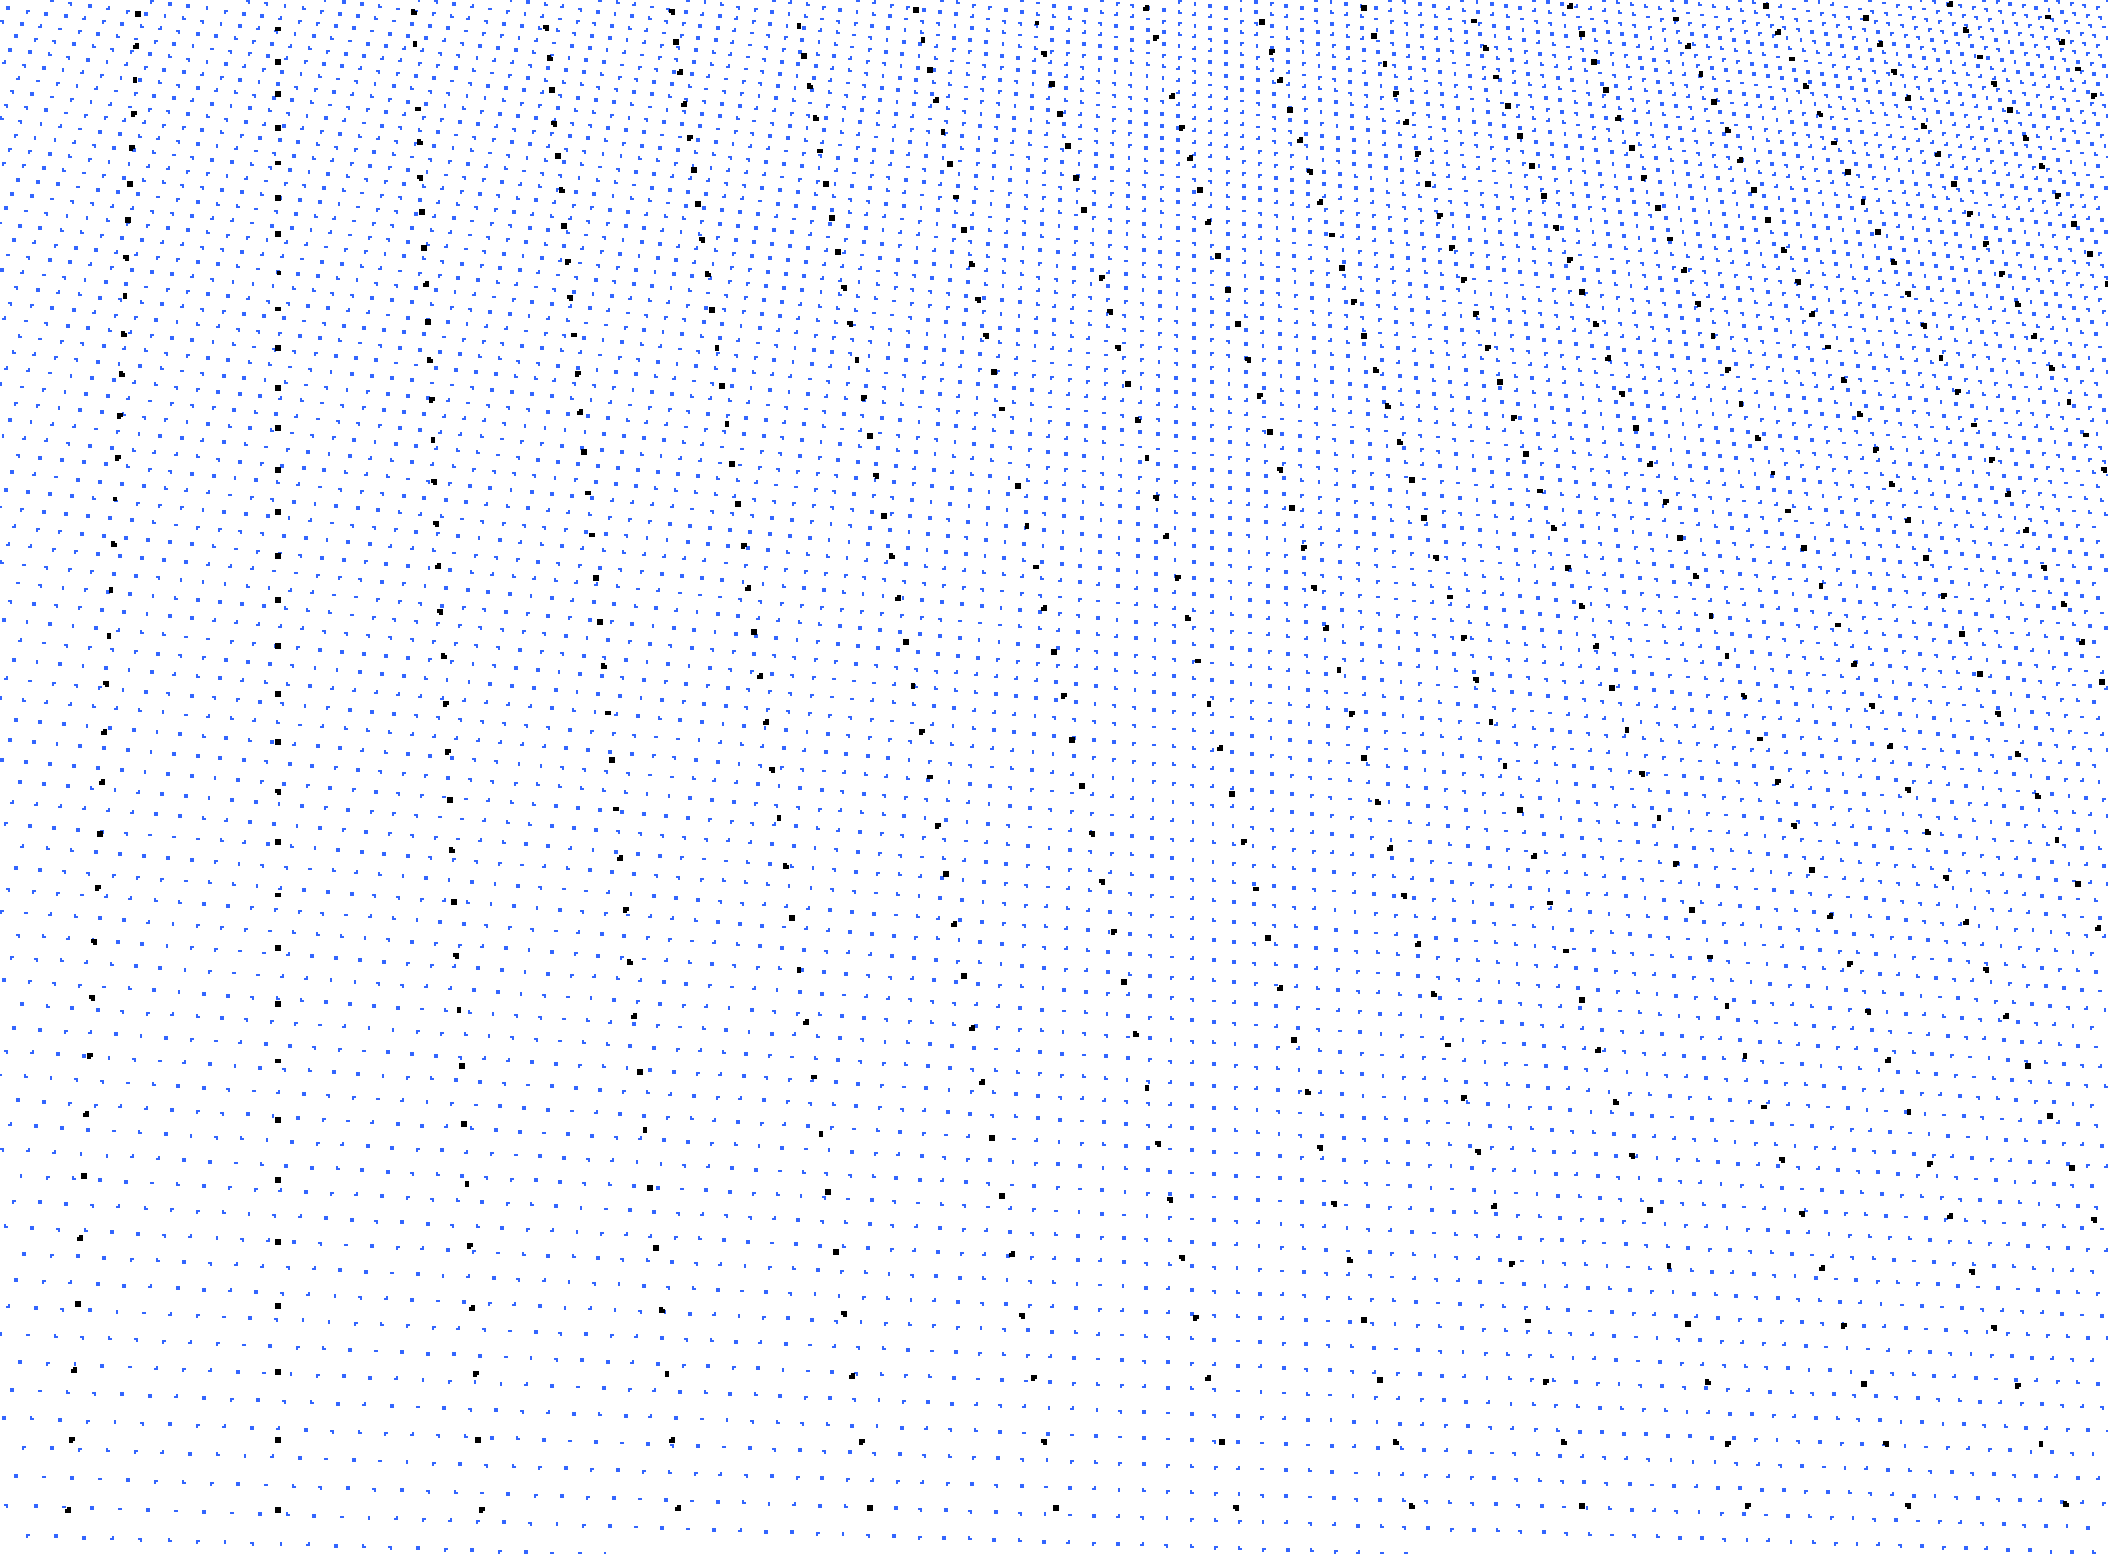
\includegraphics[width=.5\textwidth]{fig/closeup_pargrid.png}}%
}
\caption{Close-up view of parallelogram grid in $P$ (black), and sample point cloud $Q$ (blue)}
\label{fig:par_grid}
\end{figure}


\subsection{Adjusted own distance histogram}
This implies that it is possible to calculate the range of the first, linearly increasing segment of the histogram, using only the plane's normal vector $\vec{n}$ and the side length $p_l$ of the parallel projection camera. Here an attempt is made to use this result to product an \emph{adjusted own distance histogram}, which still has the initial linear increase, for point clouds that are not planes.

When the surface is no longer a plane, $\vec{n}$ will no longer be constant, but can have a different value for each point. However for smooth surfaces on the model, the normal vector will remain approximatively constant on local regions of neighboring points, as can be seen on the close-up views in the previous sections. On these planar regions the parallelogram grid point dispersion appears.

Under the assumption that most of the point clouds consists of such planar regions, its own distance histogram will be a superposition of the kinds of parallelogram grid histograms seen before, with an initial linear increasing segment.

\subsubsection{Multi-planes point cloud}
In order to test the shape of this superposition histogram, an artificially generated ``multi-planes'' point cloud is used. It consists of multiple planes places randomly in space at different orientations, projected using a parallel projection camera. An example with two planes is shown in figure \ref{fig:disks1}, shown with decreased point density.

The two planes are bounded to the shapes of disks. This does not have an effect of the histograms, and just makes the point cloud easier to visualize. If the bound was a square, it would change depending on the rotation of the plane on its own axis.

Both planes have the parallelogram grid point dispersion. The example is chosen so that one plane is approximatively facing the camera while the other is more oblique, and has a lower $\rho$ and higher $l_\text{min}$ as a result. Figure \ref{fig:multiplane_cphist} shows the own distance histograms for the two individual planes, and the superposition histogram for the entire multi-planes point cloud.

\begin{figure}[H]
\centering
\begin{subfigure}{.32\textwidth}
	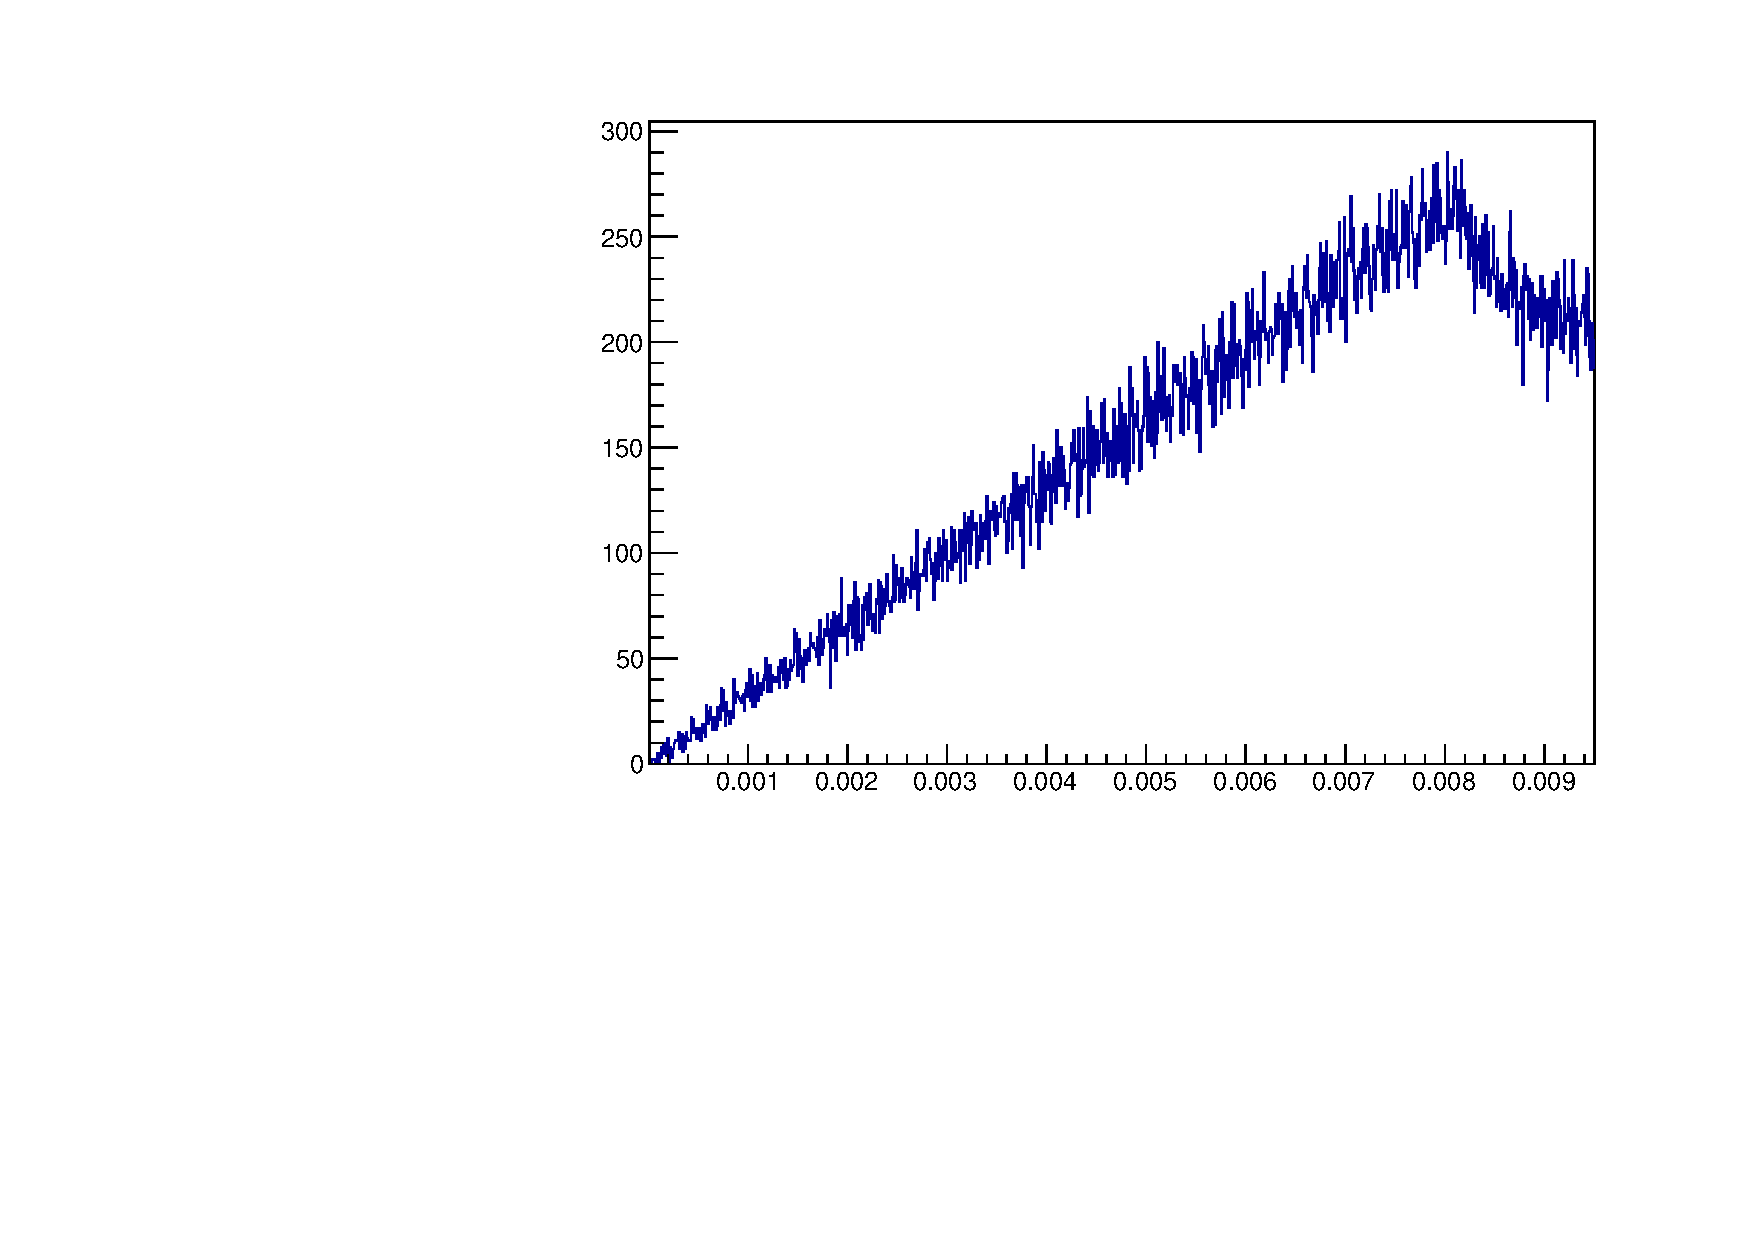
\includegraphics[width=\linewidth]{fig/orig_plane1.pdf}
	\caption{Oblique plane}
\end{subfigure}%
\begin{subfigure}{.32\textwidth}
	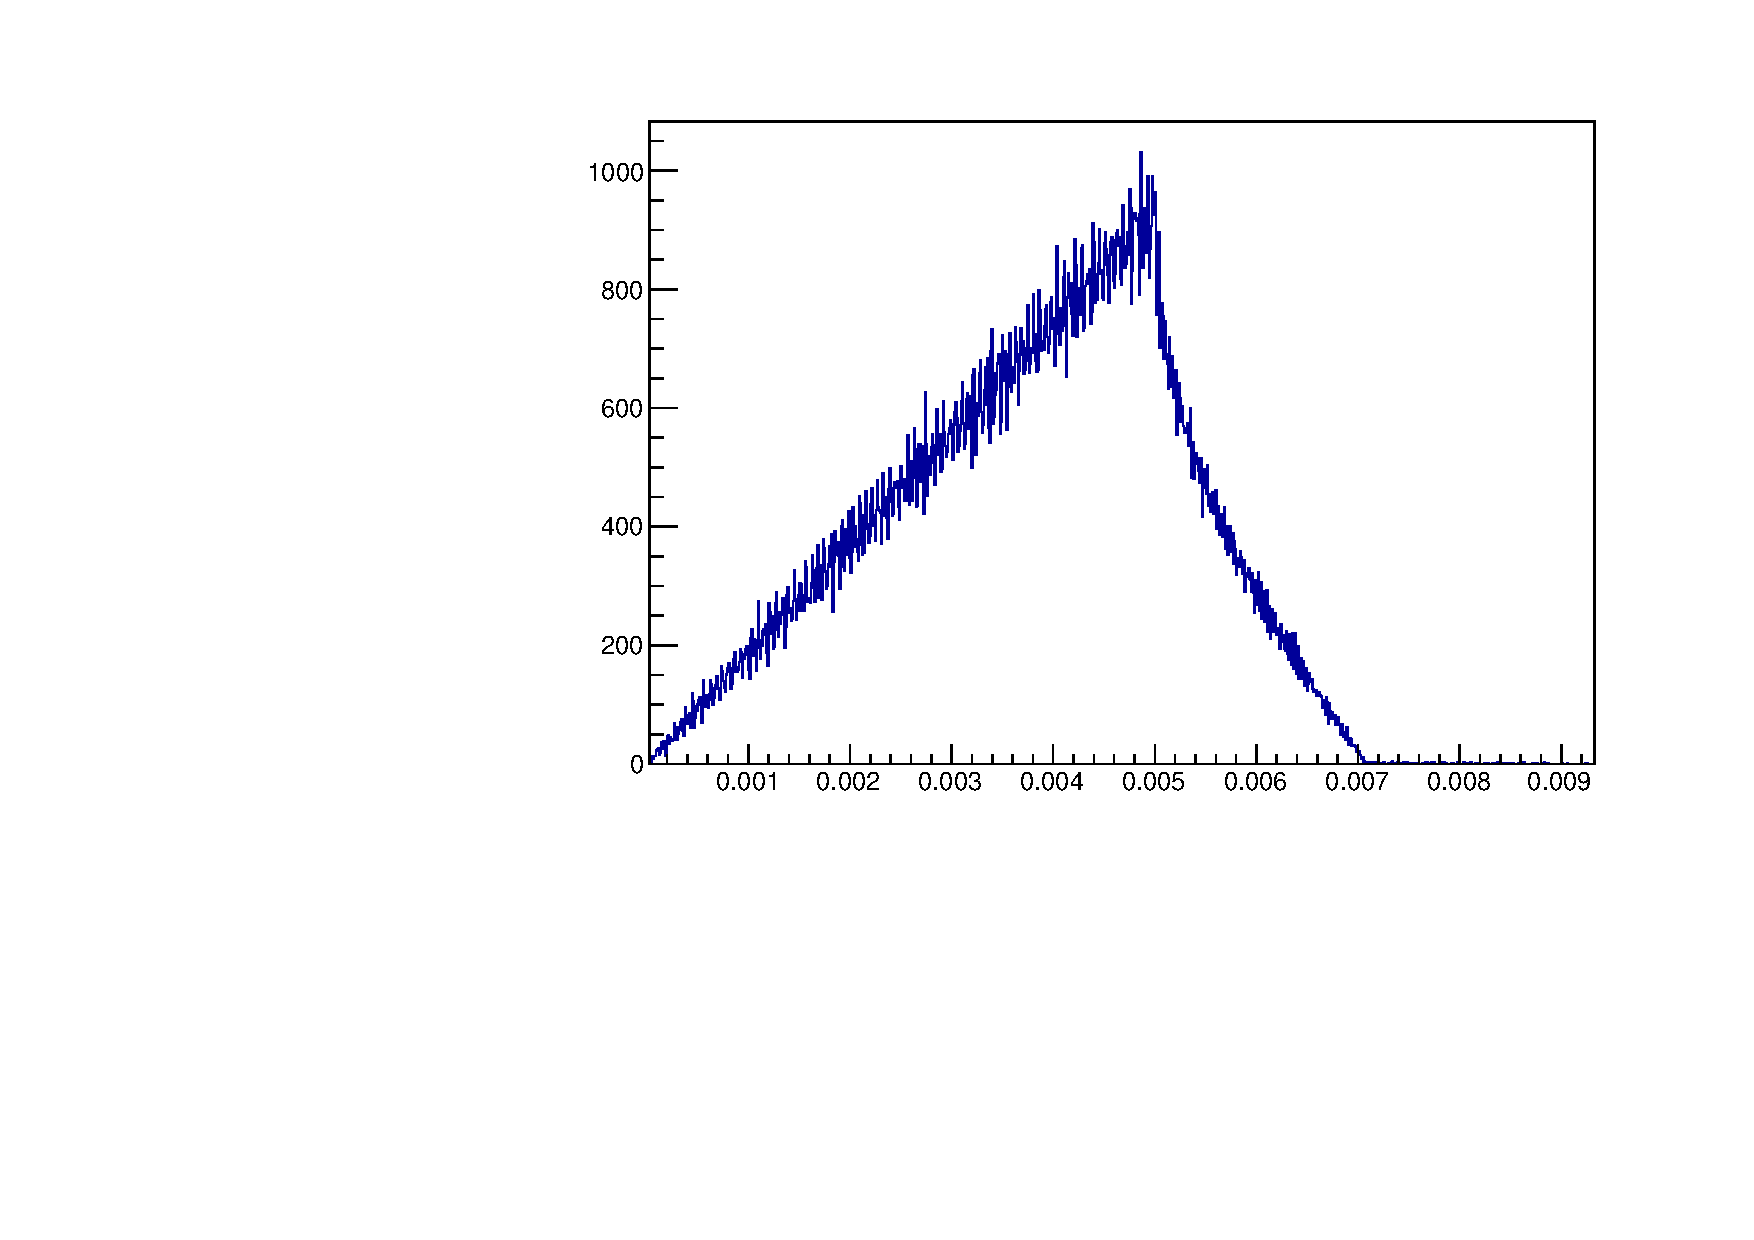
\includegraphics[width=\linewidth]{fig/orig_plane2.pdf}
	\caption{Parallel plane}
\end{subfigure}%
\begin{subfigure}{.32\textwidth}
	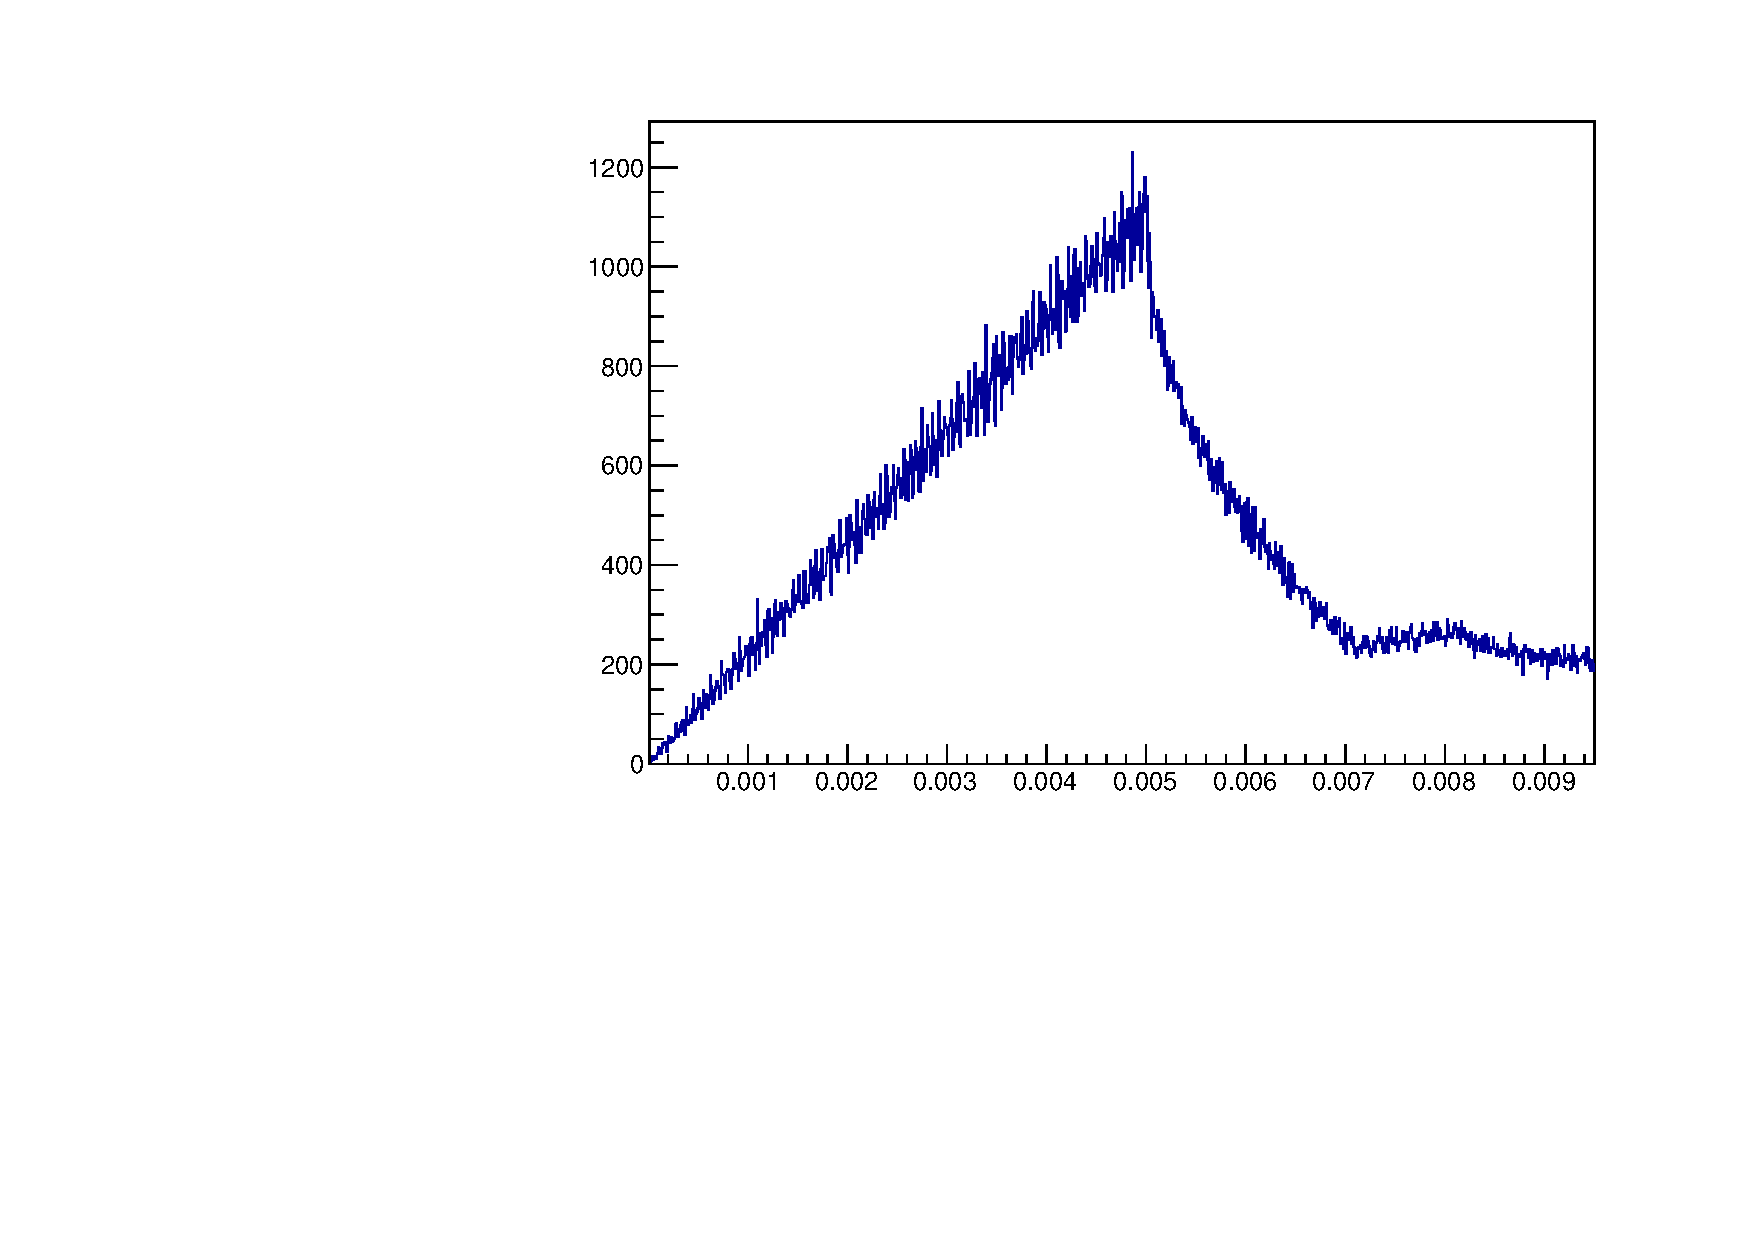
\includegraphics[width=\linewidth]{fig/orig_superposition.pdf}
	\caption{Superposition}
\end{subfigure}
\caption{Own distance histogram for disks point cloud $P$ (individual planes, and superposition)}
\end{figure}

It can be seen that the linear segment of the superposition histogram ranges up to about $0.005$, which is the minimum of the ranges on the two individual histograms. Thus the information from the remaining linear range of the oblique plane is lost.

The adjusted own distance histogram is created as follows: For each $q \in Q$, the closest point $p \in P$ is taken, for which $d = \|p - q\|$ is minimal. Then instead of $d$, the value $\frac{d}{l_{\text{min}}(\vec{n})}$ is recorded in the histogram, with a weight of $\frac{1}{\rho(\vec{n})}$.


\begin{figure}[p]
\centering
{
	\setlength{\fboxsep}{0pt}%
	\setlength{\fboxrule}{0.5pt}%
	\fbox{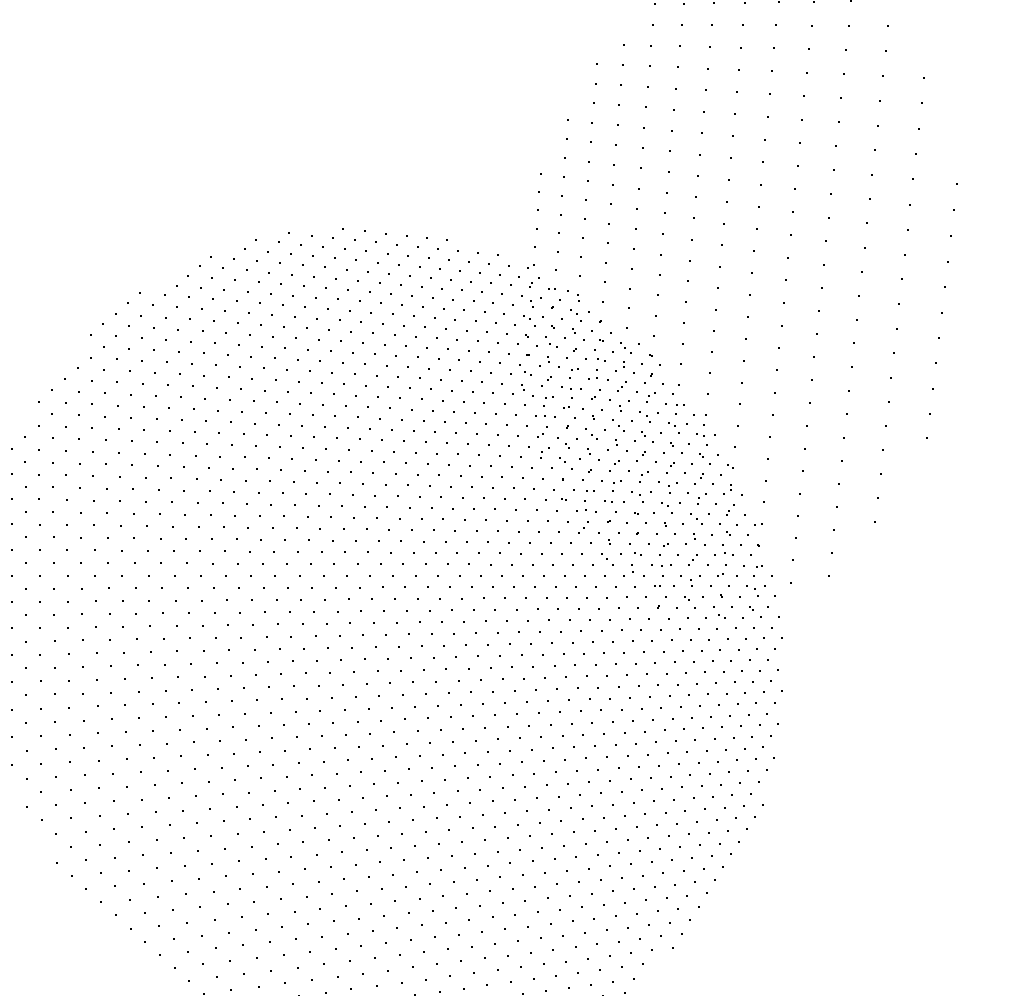
\includegraphics[width=.5\textwidth]{fig/disks1.png}}%
}
\caption{Example of multi-plane point cloud}
\label{fig:disks1}
\end{figure}

\label{fig:multiplane_cphist}
\end{figure}




\subsection{Occlusion and different bounds}
Up until now $P$ and $Q$ were considered to be perfectly aligned, constitute the same surfaces, and both have points dispersed on the whole surface at an uniform distribution. On point clouds obtained from real 3D scans this last constraint is no longer true: Parts of the surface will be occluded, and two point clouds will have different bounds.

When part of the sample point cloud $Q$ are removed



\section{Cross distance histogram}


\section{High-low density registration}
When attempting to register a short-range scan of a relatively small object with the same object in a long-range scan, the short-range point cloud will have a much higher resolution. But fine registration algorithms generally make the assumption that the two point clouds have similar resolutions. The issue of registering point clouds with different resolutions seems to be largely ignored in the literature about point cloud registration algorithms.

\subsection{First experiment}
A first observation is that in general for ICP, lowering the resolution of the loose point cloud does not much reduce the accuracy of the registrations. This is shown in experiment \ref{sec:ex_bunny_hilo} (see appendix), in which the Stanford Bunny model is fine registered with a lower density copy of itself. Let $P$ be the fixed point cloud and $Q$ the (downsampled) loose point cloud.

The most basic variant of ICP is used: All points are selected, correspondences from are taken $Q$ to $P$ by the closest point criterion, no correspondences are rejected, weights are uniform, and the point-to-point error metric is used. The copies are made in such a way that they never have two points in common: $P$ is constructed by taking randomly chosen $50\%$ of the points from the original model, and $Q$ is constructed from the remaining $50\%$. After this $Q$ is randomly downsampled by $60$ different amounts.

The experiment is done in three instances. For the first one (figure \ref{fig:bunny_globmin}), $P$ and $Q$ start out perfectly aligned, and for the two other ones (figures \ref{fig:bunny_globsmall} and (figure \ref{fig:bunny_globmed})), they start out with a small (or larger) random initial transformation. $40$ iterations of the registration algorithm are run and the final errors are recorded.

The plots show the error measured using the mean unsigned distances of the true correspondences, as defined in section \ref{sec:lm_known_ttrans}. It is zero if and only if $P$ and $Q$ are perfectly aligned. The X axis indicates the ratio of the number of points $\frac{\|Q\|}{\|P\|}$.


\subsubsection{Analysis}
Two things can be observed: The final error does not depend much on the downsampling level, and the error always converges to about $0.001$, even when $P$ and $Q$ were perfectly aligned to start with.

To define a rigid transformation, three pairs of corresponding points are sufficient as long as the three points do not lie on the same plane. (see section \ref{sec:lsq_align}) So even when $Q$ is reduced to three points the point-to-point error metric can be minimized. RANSAC-based approaches to registration, such as 4PCS are based on this.

Figure \ref{ref:bunny_hilo_ev} shows how the true error evolves during the $40$ executions of ICP on the first experiment without initial displacement. $P$ and $Q$ were generated to have no common points. When choosing the points closest to the true corresponding point instead, the error does not cancel out completely, and thus the correct alignment is no longer the global minimum of the error metric.

Figure \ref{bunny_first_tcor} shows the state after the registration. $Q$ is rendered in blue color and $P$ in red. From each point $q_i \in Q$ a line segment towards the true corresponding point $q'_i$ is shown, which is not a point $p_i \in P$. On this part $Q$ has from the correct alignment deviated towards the right.

\begin{figure}[p]
\centering
{
	\setlength{\fboxsep}{0pt}%
	\setlength{\fboxrule}{0.5pt}%
	\fbox{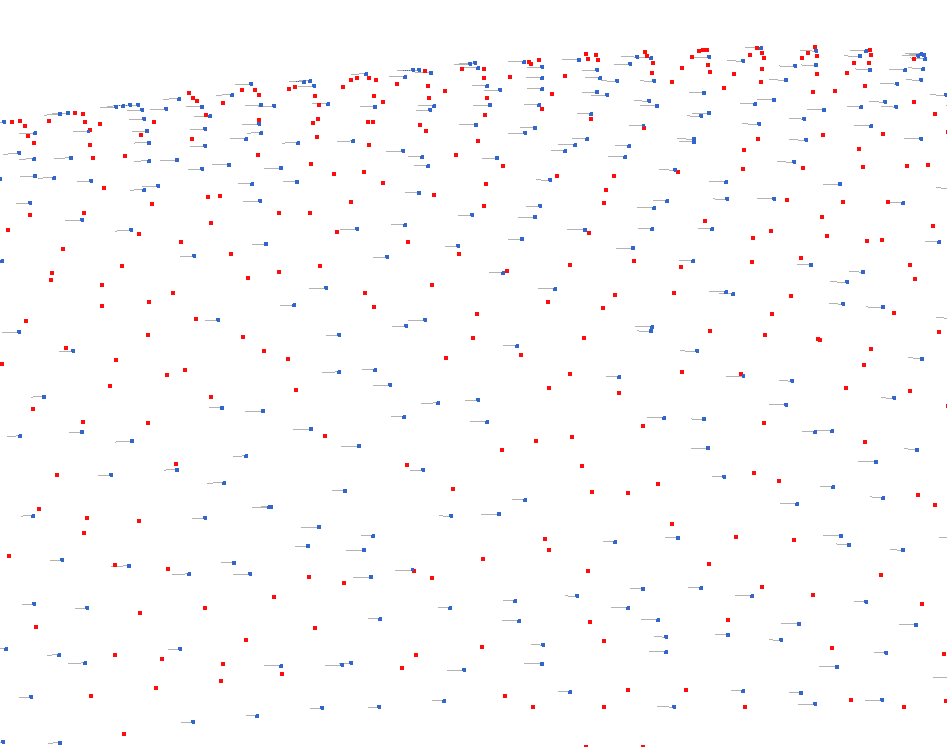
\includegraphics[width=.7\textwidth]{fig/bunny_first_tcor.png}}
}
\caption{Bunny model registered to itself, true correspondences shown}
\label{fig:bunny_first_tcor}
\end{figure}

When $\forall q_i, p_i = q'_i$, the correct alignment would be found. When $P$ and $Q$ are already aligned, $q_i = q'_i$. Figure \ref{fig:bunny_fexp_before} shows the histogram of $\|q'_i - p_i\| = \|q_i - p_i\|$ for the case when $50\%$ (or $80\%$) of the model points are taken for $P$ and the remaining for $Q$, and no additional downsampling is applied.

\begin{figure}[h]
\centering
\begin{subfigure}{.5\textwidth}
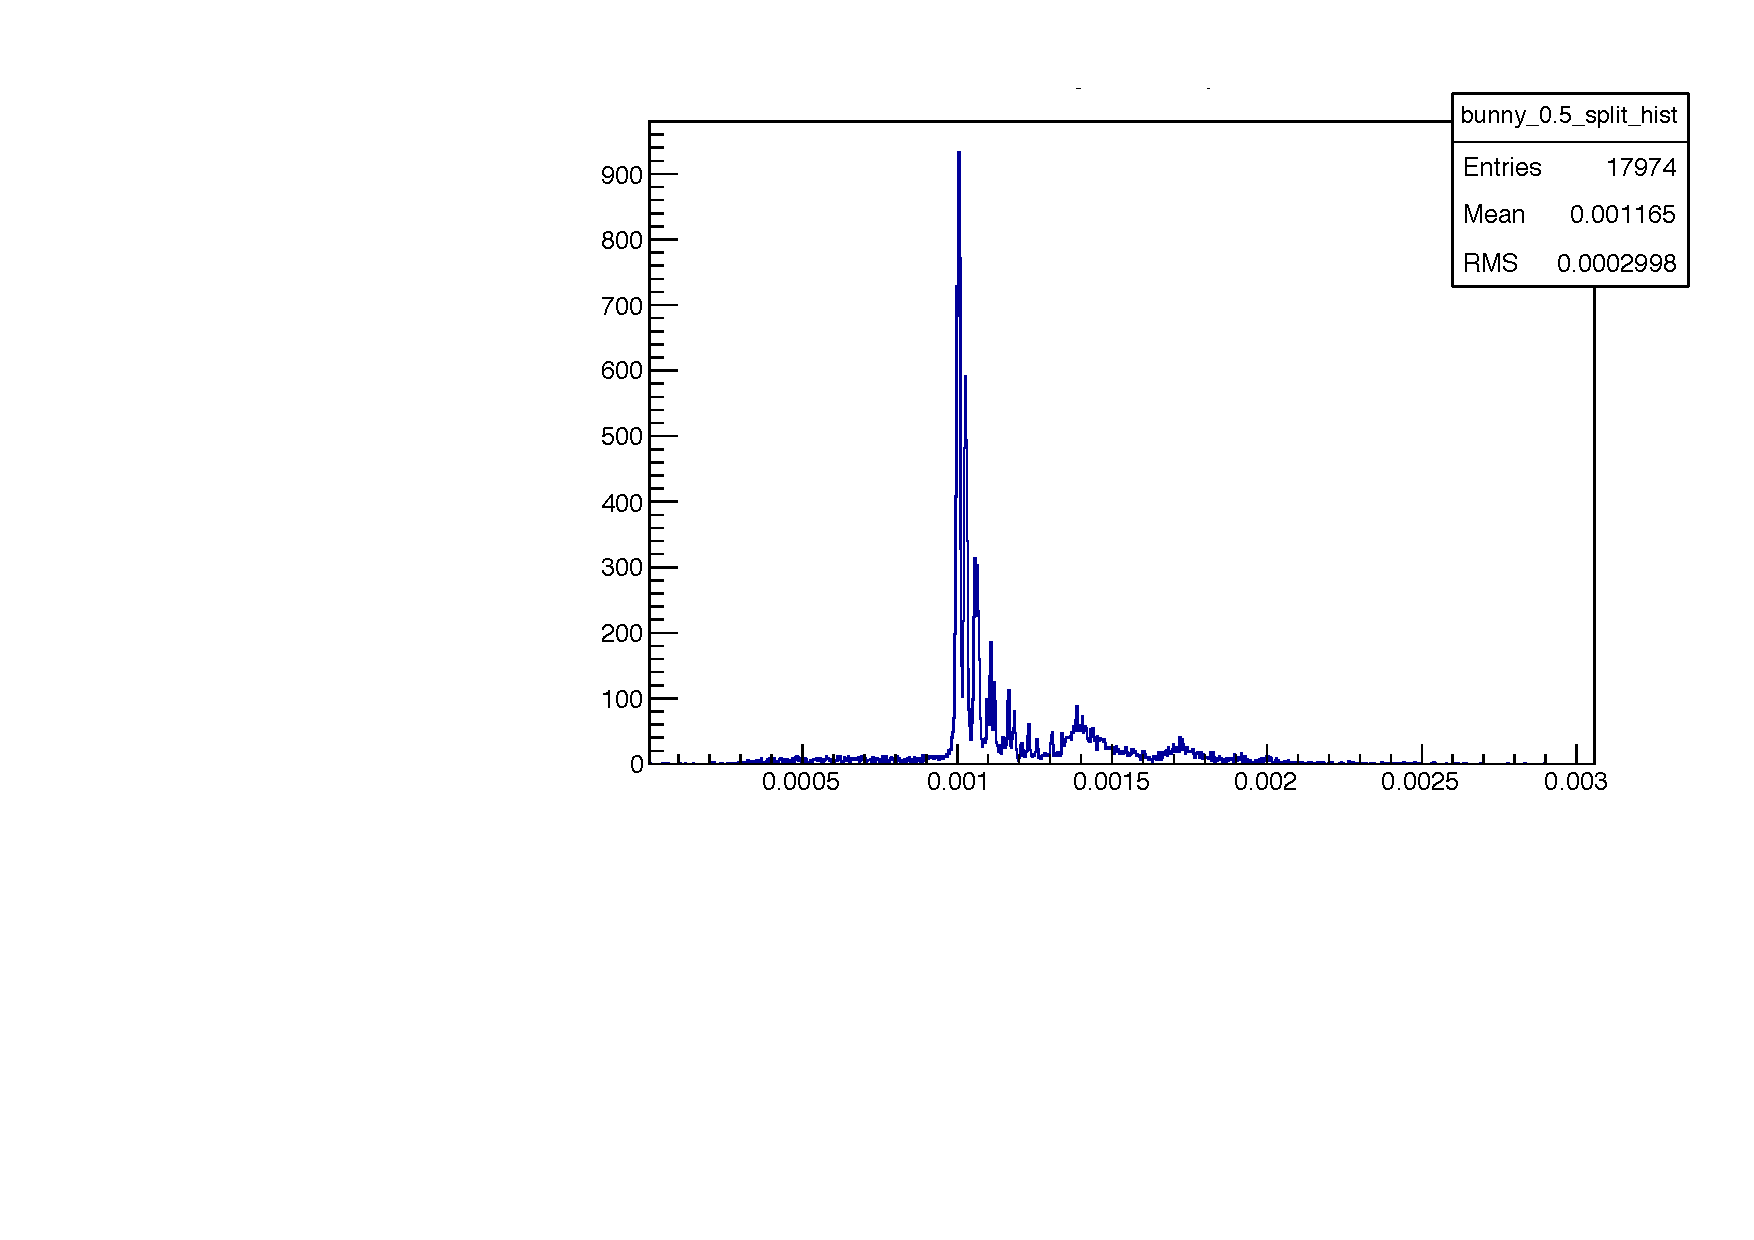
\includegraphics[width=\linewidth]{fig/bunny_05_split.pdf}
\end{subfigure}%
\begin{subfigure}{.5\textwidth}
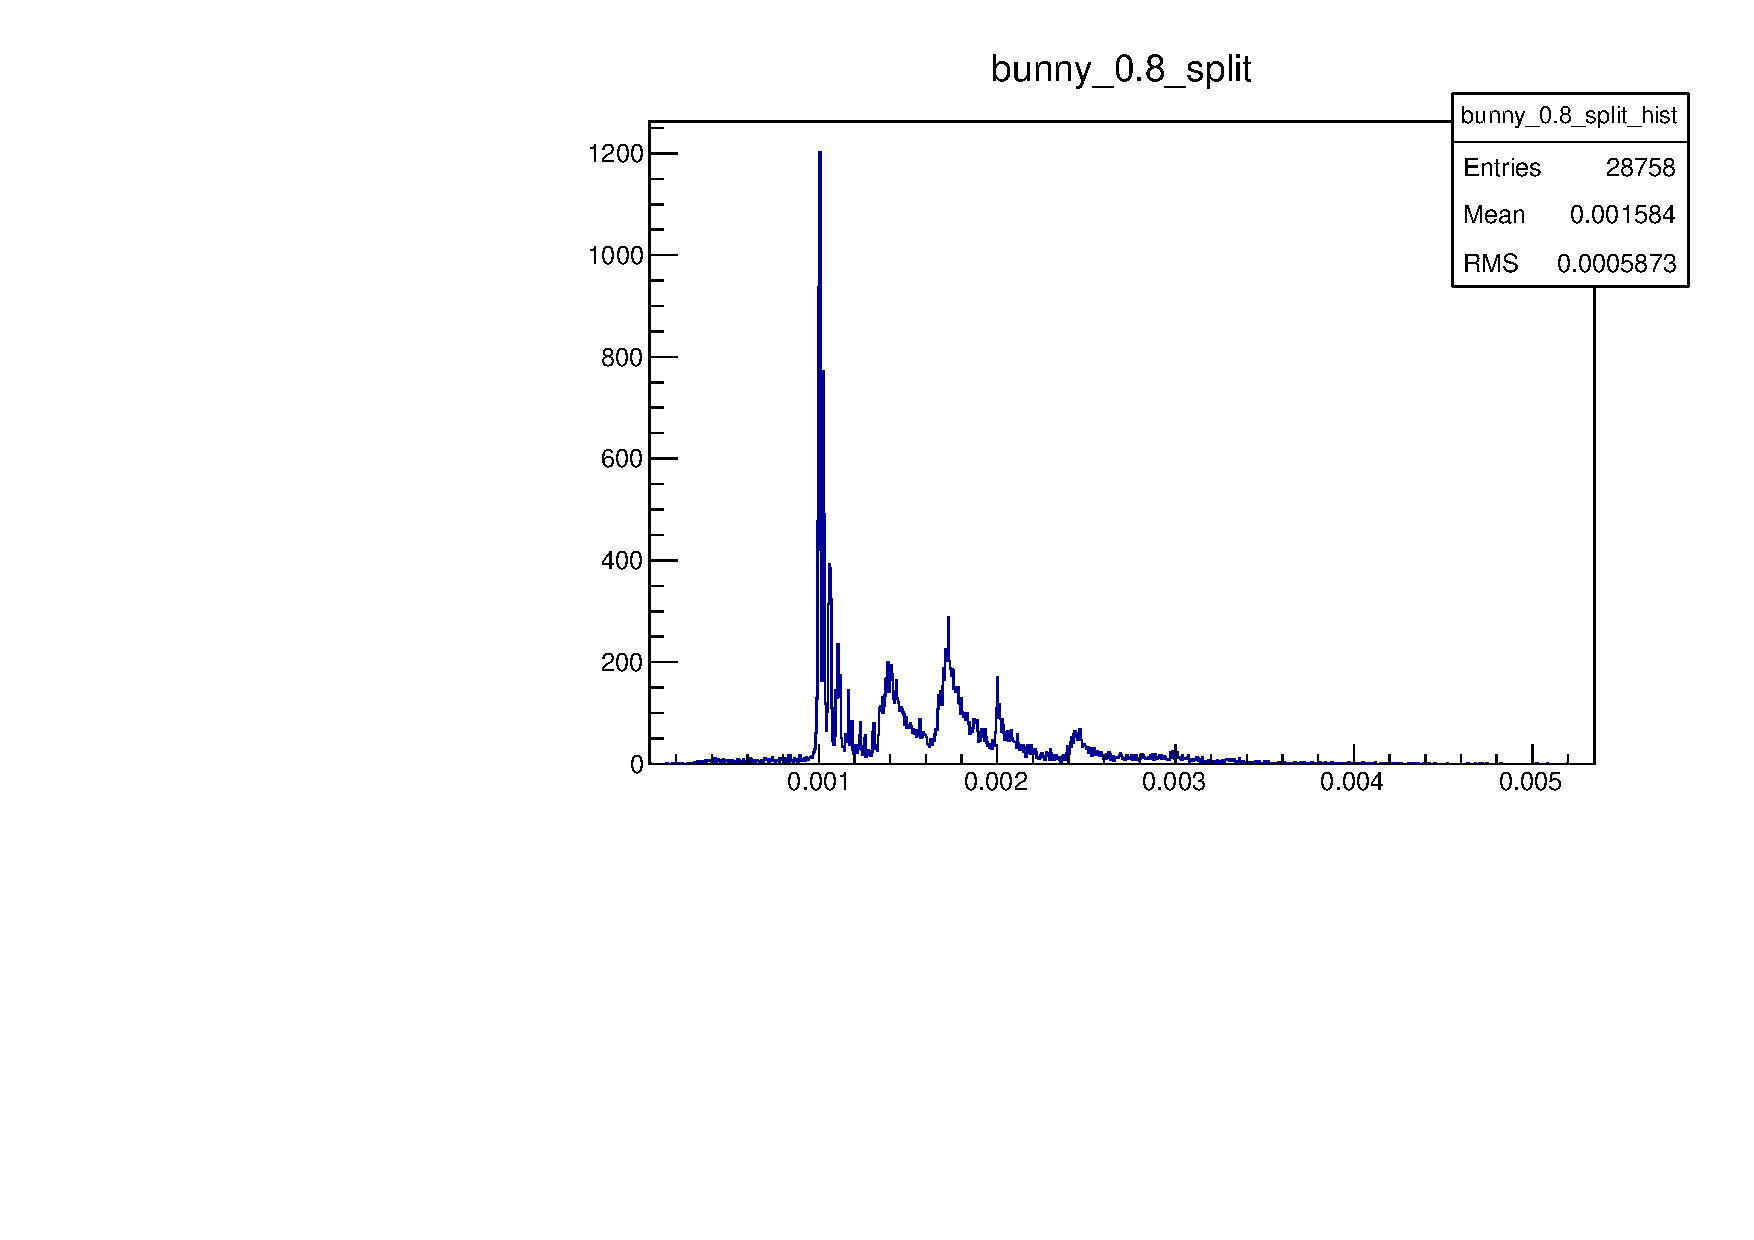
\includegraphics[width=\linewidth]{fig/bunny_08_split.pdf}
\end{subfigure}
\caption{Histograms of $\|q_i - p_i\|$ for 50\% and 80\% split}
\label{fig:bunny_fexp_before}
\end{figure}

In both cases, $\| q - p \| \approx 0.001$ is a mode in the distribution. Smaller values are infrequent. Additional spikes occur for some values above $0.001$. 

The reason is that for the original Bunny point clouds, the points are evenly distributed on the surface on an approximatively square grid, with a mean distance of about $0.001$ between adjacent points, as seen in the close-up view in figure \ref{fig:bunny_grid_closeup}. Figure \ref{fig:bunny_closest} shows a histogram made by taking from each point $p$ on the Bunny point cloud $B$, the closest point $p' \in B$ with $p' \neq p$. In the closest point histograms from $Q$ to $P$, any point that is in $Q$ is missing in $P$ and hence the closest point is often the one at a distance of $0.001$. Some instances appear where this point is not in $P$ either, so the closest point is further. This explains the spike at $0.002$. The other spikes occur when the closest point is in a diagonal direction on the grid. This ``grid'' is approximate and the surface is embedded in a non planar way in 3D space, so most samples do not fall exactly in one of these spikes.

For the true correspondences, the histogram would be a single spike at $\|p_i - q'_i\| = 0$. 



\subsection{Experiments on relief}



\subsection{Limits of accuracy}




\subsection{Metric for resolution}
Informally, the resolution of a point cloud indicates how many samples (i.e. points) of the represented object is contains. For a range image taken by a 3D scanner, the resolution is defined with its width and height, which correspond to the number of measurements taken per scan line and the number of scan lines, for its whole field of view.

The assumption was made that the points in the point cloud lie on a set ensemble of two-dimensional surfaces, which are embedded in three-dimensional space. A points density measure in terms of number of points per unit of volume is thus not meaningful. Instead the \emph{density} of the distribution of points on a surface area if used.




\section{Separation of large scans}

\section{Variable density}
